\documentclass[czech, bp, kiv, he, iso690numb, pdf]{fasthesis}
\usepackage{enumitem}
\usepackage{subcaption} 
\usepackage{url}
\usepackage{xcolor}
\usepackage{hyperref}
\usepackage{dirtree}


\renewcommand{\UrlBreaks}{\do\.\do\_\do\/\do\(\do\)}
\title{Mobilní aplikace pro inzerci a adopci domácích zvířat}
\author{Adam}{Míka}{}{}
\supervisor{Ing. Martin Zíma, Ph.D.}
\stagworkid{100717}
\assignment{zadani.pdf}
\signdate{5}{5}{2025}{V Plzni}
\addbibresource{bib.bib}
\abstract{Tato bakalářská práce se zabývá návrhem a implementací mobilní aplikace pro inzerci a adopci domácích zvířat. Práce analyzuje existující softwarová řešení v této oblasti a identifikuje jejich nedostatky. Na základě provedené analýzy je navržena nová aplikace, která umožňuje efektivní propojení zájemců o adopci s útulky nabízejícími zvířata. Aplikace je implementována pomocí technologií React Native a Expo pro frontend a Appwrite pro backend. Výsledkem je multiplatformní mobilní aplikace s intuitivním uživatelským rozhraním, která nabízí funkce jako procházení katalogu zvířat, pokročilé filtrování, označování oblíbených položek a správu zvířat pro útulky. Práce popisuje celý proces vývoje od analýzy požadavků přes návrh architektury až po implementaci a testování. Součástí práce je také zhodnocení výsledného řešení a návrh možných budoucích rozšíření.}
{This bachelor thesis focuses on the design and implementation of a mobile application for pet advertising and adoption. The thesis analyzes existing software solutions in this area and identifies their shortcomings. Based on the conducted analysis, a new application is designed that enables effective connection between potential adopters and shelters offering animals. The application is implemented using React Native and Expo technologies for the frontend and Appwrite for the backend. The result is a cross-platform mobile application with an intuitive user interface, offering features such as browsing an animal catalog, advanced filtering, marking favorites, and animal management for shelters. The thesis describes the entire development process from requirements analysis through architecture design to implementation and testing. The work also includes an evaluation of the resulting solution and suggestions for possible future extensions.}
\keywords{Mobilní aplikace, iOS, Android, Realtime databáze}
\acknowledgement{Tímto bych rád poděkoval Ing. Martinovi Zímovi Ph.D. za odborné vedení, cenné rady, věcné připomínky a vstřícnost při konzultacích a vypracovávání bakalářské práce.
\begin{flushright}
\textit{Adam Míka},\\
autor práce\\
(duben 2025)
\end{flushright}
}


\begin{document}
\frontpages[tm]
\tableofcontents

\chapter{Úvod}
V současné době moderních technologií hrají mobilní aplikace klíčovou roli v mnoha aspektech každodenního života. Jednou z oblastí, kde mohou tyto technologie přinést výrazný přínos, je péče o domácí zvířata. Téma adopce a inzerce domácích zvířat je stále aktuálnější, přičemž potřeba inovativních řešení je více než zřejmá. Rostoucí počet opuštěných zvířat v útulcích a zájem o odpovědné vlastnictví zvířat vyžadují efektivní nástroje pro propojení zájemců o adopci s majiteli zvířat.

Cílem této práce je návrh a realizace mobilní aplikace, která bude sloužit jako moderní a uživatelsky přívětivá platforma pro inzerci a adopci domácích zvířat. Vytvořená aplikace bude uživatelům umožňovat snadné prohlížení inzerátů a filtrování podle specifických kritérií (například druhu zvířat, lokace nebo věku). Kromě toho nabídne intuitivní uživatelské rozhraní, které bude snadno ovladatelné i pro méně technicky zdatné uživatele.

Analýza stávajících řešení ukazuje, že dostupné aplikace často nevyhovují požadavkům moderních uživatelů. Mnoho z nich postrádá klíčové funkce nebo je orientováno pouze na webové prostředí. Tyto nedostatky ztěžují proces adopce a snižují efektivitu stávajících platforem. Navržená aplikace se zaměří na odstranění těchto nedostatků a nabídne komplexní řešení, které bude reflektovat potřeby cílové skupiny.

Motivací pro tuto práci je nejen zlepšení procesu adopce zvířat, ale také zvýšení povědomí o odpovědném vlastnictví domácích zvířat. Mobilní aplikace jako centralizovaný nástroj umožní propojení uživatelů s databázemi útulků, zjednoduší správu inzerátů a podpoří snahu o nalezení vhodného domova pro zvířata v nouzi. Výsledkem práce bude funkční aplikace, jejíž struktura a možnosti budou navrženy s ohledem na další rozšíření, jako je například integrace s veterinárními službami nebo sociálními sítěmi.

Tato práce si klade za cíl nejen vyvinout funkční produkt, ale také přispět k řešení společenského problému a ukázat, jak lze moderní technologie využít pro podporu dobré věci.

\chapter{Analýza existujících řešení}

Tato kapitola je zaměřena na analýzu dostupných softwarových řešení, která se specializují na inzerci a adopci domácích zvířat. Cílem této analýzy je prozkoumat funkce, uživatelské rozhraní a přístupy jednotlivých aplikací, identifikovat jejich výhody a nevýhody a na základě získaných poznatků formulovat doporučení pro návrh nové aplikace.

Analýza zahrnuje webové i mobilní aplikace, které slouží k podobným účelům, jako je zamýšlený projekt. Pro hodnocení aplikací byly zvoleny následující kritéria:
\begin{itemize}
    \item Rozsah a kvalita nabízených funkcí (např. vyhledávání zvířat, proces adopce, registrace útulků).
    \item Uživatelská přívětivost a intuitivnost rozhraní.
    \item Celkový přínos pro cílovou skupinu uživatelů.
    \item Technologická řešení a možnosti rozšiřitelnosti aplikace.
\end{itemize}
Následující sekce detailně rozebírají jednotlivé vybrané aplikace. Hodnocení se zaměřuje na klíčové aspekty, jako je funkčnost a uživatelský zážitek, a následně je doplněno shrnutím hlavních zjištění.

\section{Přehled dostupných softwarových řešení}

V oblasti adopcí a inzercí domácích zvířat existuje řada softwarových řešení, která se liší svou zaměřeností, funkcionalitou a cílovou skupinou uživatelů. Tato řešení lze rozdělit do kategorií zahrnujících webové portály a mobilní aplikace. Následující přehled shrnuje klíčové vlastnosti vybraných softwarových řešení.

\subsection{Webové portály}

V následující části jsou popsány webové portály, které hrají významnou roli v oblasti adopce a inzerce domácích zvířat. Jedná se o české i zahraniční platformy zaměřené na propojení útulků se zájemci o adopci, přičemž každá z nich nabízí specifické funkce a přístupy.

\begin{itemize}
    \item \textbf{Pesweb} -- Tento český portál se zaměřuje na inzerci psů a koček k adopci. Umožňuje uživatelům vyhledávat zvířata podle specifických parametrů, jako je věk, velikost nebo plemeno. Důležitou funkcí je také možnost přímého kontaktu s útulky prostřednictvím platformy. Mezi hlavní výhody patří přehlednost a jednoduchost uživatelského rozhraní.

    \item \textbf{Voriskov} -- Online útulek rozšiřující nabídku i na další druhy domácích mazlíčků, jako jsou hlodavci nebo ptáci. Portál nabízí uživatelsky přívětivé prostředí, ale jeho nabídka se primárně zaměřuje na psy. Jedná se o jednoduchý a intuitivní systém vhodný pro široké spektrum uživatelů.

    \item \textbf{Dog-point} -- Webový portál specializovaný výhradně na adopci psů. Nabízí podrobné profily zvířat, které zahrnují informace o jejich zdravotním stavu, povahových rysech a základních požadavcích na péči. Portál se zaměřuje na přehlednou prezentaci informací a efektivní propojení zájemců s útulkem.

    \item \textbf{Puppio} -- Český webový portál zaměřený na inzerci domácích mazlíčků. Portál se specializuje výhradně na inzerce zvířat ze Středočeského kraje. Jedná se o regionálně orientovanou platformu, která klade důraz na jednoduché uživatelské prostředí a základní vyhledávací funkce.

    \item \textbf{Anidef} -- Online webový útulek zaměřený na adopce nejen psů a koček, ale i dalších druhů zvířat, jako jsou kozy, krávy, králíci nebo holubi. Platforma poskytuje základní informace o zvířatech nabízených k adopci, včetně věku, plemene a aktuálního zdravotního stavu. Portál neobsahuje pokročilé funkce ani integrovaný systém pro správu adopcí, jeho hlavním cílem je však rozšíření možností adopce na širší spektrum zvířat.
\end{itemize}

Webové portály popsané výše představují důležitou součást ekosystému adopce domácích zvířat. Každý z nich je charakteristický svým zaměřením a přístupem k řešení potřeb uživatelů. Přestože nabízejí širokou škálu funkcí, identifikovány byly i určité mezery, které budou dále rozebrány v detailní analýze.

\subsection{Mobilní aplikace}
\textbf{Petfinder} – Mobilní aplikace, která propojuje zájemce o adopci s útulky v Severní Americe. Nabízí pokročilé vyhledávací funkce a personalizovaná doporučení, avšak její dostupnost je geograficky omezená pouze na tento region.

Tento přehled poskytuje základní orientaci v dostupných řešeních. Zároveň ukazuje, že stávající nabídka aplikací a portálů je často omezena na specifické funkce nebo geografická území, což otevírá prostor pro inovativní a komplexnější přístup k problematice adopce domácích zvířat. V následujících částech se budeme věnovat detailní analýze těchto řešení.

\section{Detailní analýza vybraných aplikací}

Tato část práce se podrobně zabývá analýzou jednotlivých aplikací zaměřených na adopci domácích zvířat. Výběr zahrnuje jak české aplikace, například \textbf{Pesweb} nebo \textbf{Anidef}, tak zahraniční platformy jako \textbf{Petfinder}. Cílem této analýzy je zhodnotit jejich funkce, uživatelské rozhraní a celkový přínos pro uživatele.

Každá aplikace bude stručně představena, následně budou uvedeny její hlavní výhody a nevýhody. Součástí analýzy budou i vizuální ukázky aplikací ve formě přiložených snímků obrazovek nebo uživatelských rozhraní. Tyto ukázky napomohou ilustrovat klíčové aspekty, jako je přehlednost a intuitivnost designu. 

\noindent Hodnocení bude rozděleno do následujících kategorií:

\noindent\textbf{Funkčnost}: Nabízené funkce, jejich rozsah a přizpůsobení potřebám uživatelů.

\noindent\textbf{Uživatelské rozhraní}: Přehlednost, jednoduchost a estetika designu.

\noindent\textbf{Technologická řešení}: Použité technologie, možnosti integrace a rozšiřitelnost.

\noindent\textbf{Regionální dostupnost}: Geografická omezení a přístupnost pro uživatele.

\pagebreak
\subsection{Pesweb}

\noindent \textbf{Funkčnost}: Portál nabízí možnost vyhledávání zvířat podle různých parametrů, jako jsou věk, velikost či plemeno, a umožňuje přímou komunikaci s útulky. Přesto postrádá pokročilé funkce, jako je personalizace vyhledávání na základě uživatelských preferencí nebo automatizace adopčního procesu, což omezuje jeho komplexnost.\\

\noindent \textbf{Uživatelské rozhraní}: Uživatelské rozhraní je navrženo jednoduše a intuitivně, což usnadňuje jeho využívání i méně technicky zdatným uživatelům. Některé grafické prvky by však mohly být upraveny tak, aby lépe odpovídaly požadavkům uživatelů na moderní vizuální přehlednost a estetiku \cite{fluffy}\cite{petfood}. Navíc chybějící optimalizace pro mobilní zařízení může uživatelům s menšími obrazovkami způsobovat komplikace při navigaci po portálu.\\

\noindent\textbf{Technologická řešení}: Portál funguje pouze ve webovém prostředí a nenabízí podporu mobilních aplikací. Výkon systému je pomalý, zejména při přepínání mezi sekcemi, což může negativně ovlivnit uživatelský zážitek.\\

\noindent \textbf{Regionální dostupnost}: Platforma je zaměřena výhradně na Českou republiku, přičemž poskytuje pokrytí po celé zemi. Tento přístup podporuje dostupnost zvířat z regionálních útulků pro zájemce o adopci.\\

\begin{figure}[h!]
    \centering
    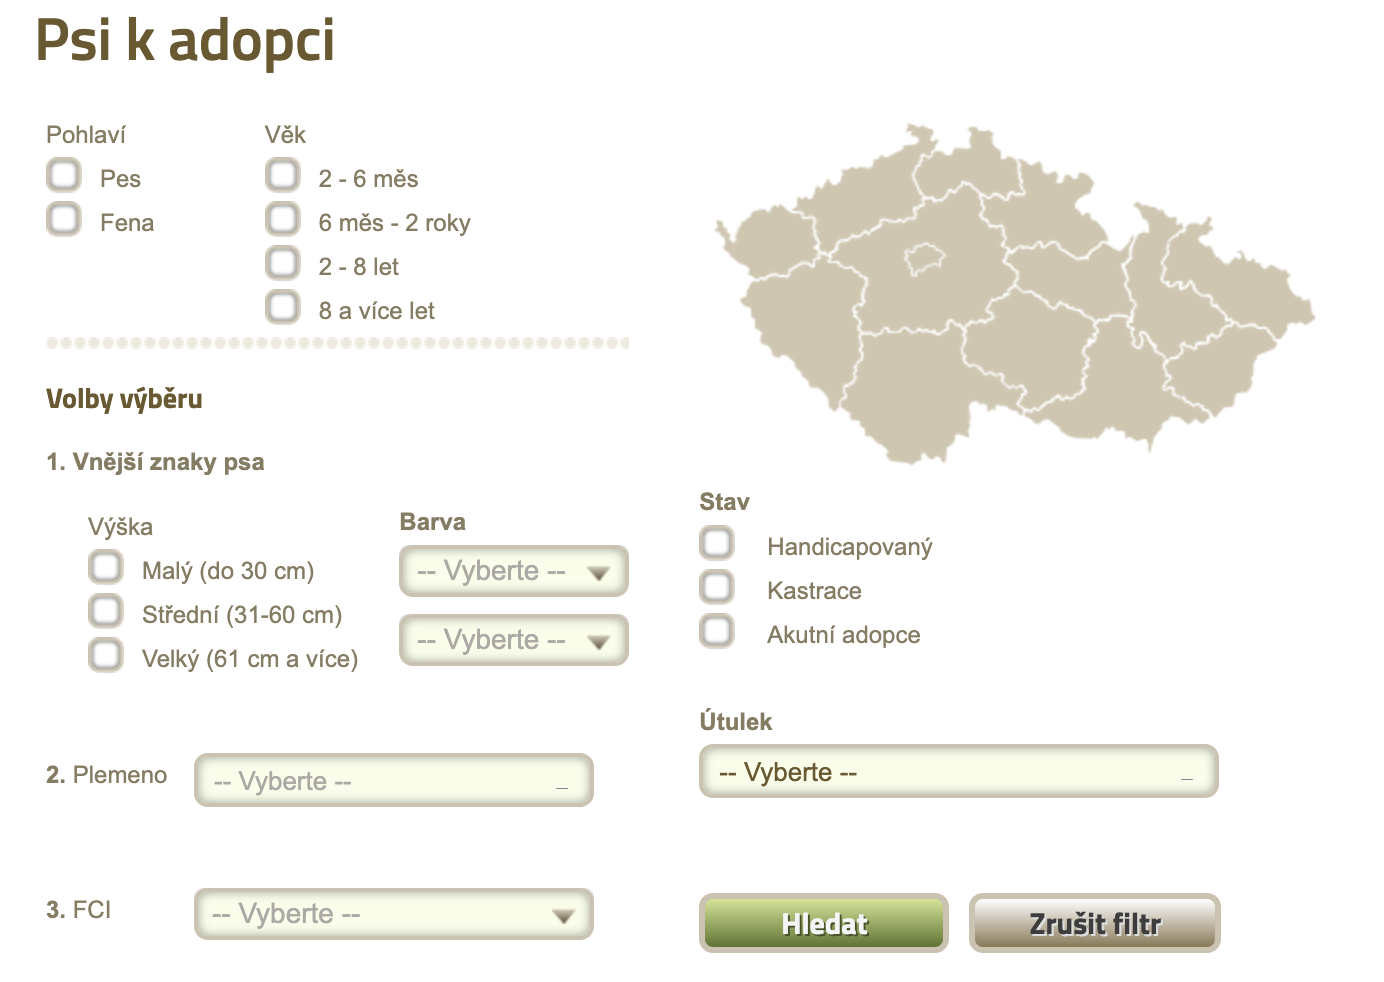
\includegraphics[width=1\textwidth]{img/pesweb.png} % Cesta k obrázku
    \caption{Filtrace záznamů na portále Pesweb} % Popis obrázku
    \label{fig:pesweb_filter} % Identifikátor pro odkazování na obrázky
\end{figure}

\newpage

\subsection{Anidef}

\noindent \textbf{Funkčnost}: Platforma poskytuje základní informace o zvířatech, včetně věku, plemene a zdravotního stavu. Nicméně postrádá pokročilé adopční funkce, jako je personalizace na základě preferencí uživatele, možnost sledování adopcí nebo filtrování podle kritérií, jako jsou plemeno, velikost či věk, což omezuje její praktičnost.\\

\noindent\textbf{Uživatelské rozhraní}: Rozhraní je jednoduché a uživatelsky přívětivé, což zajišťuje snadnou orientaci pro většinu uživatelů. Některé aspekty grafického návrhu by však mohly být upraveny tak, aby lépe odpovídaly očekáváním uživatelů preferujících vizuálně propracovanější aplikace \cite{fluffy}\cite{petfood}, což by mohlo zvýšit jeho atraktivitu pro mladší uživatele.\\

\noindent\textbf{Technologická řešení}: Platforma je dostupná výhradně jako webový portál, což omezuje její využití na mobilních zařízeních, jelikož chybí nativní mobilní aplikace nebo integrace s dalšími systémy. Proces adopce je realizován prostřednictvím Google formuláře, jehož délka a struktura mohou být pro některé zájemce méně přívětivé.\\

\newpage
 
\noindent \textbf{Regionální dostupnost}: Služby jsou geograficky omezeny na Českou republiku a vztahují se pouze k určitému konkrétnímu útulku, což snižuje jejich flexibilitu pro uživatele z jiných regionů.\\


\subsection{Petfinder}

\noindent \textbf{Funkčnost}: Aplikace nabízí pokročilé vyhledávací funkce, včetně možnosti filtrování zvířat podle druhu, věku nebo lokality. Kromě toho obsahuje personalizovaná doporučení na základě uživatelských preferencí, což zlepšuje uživatelský zážitek.\\

\noindent \textbf{Uživatelské rozhraní}: Uživatelské rozhraní je jednoduché a funkční, avšak některé designové prvky by mohly být optimalizovány, aby lépe odpovídaly očekáváním uživatelů v oblasti pohodlného a plynulého ovládání \cite{fluffy}\cite{petfood}. Určité nedostatky mohou snižovat celkový uživatelský zážitek, zejména při použití na mobilních zařízeních.\\

\noindent \textbf{Technologická řešení}: Aplikace využívá geolokaci a algoritmy pro personalizaci doporučení, což ji činí technologicky vyspělou. Její využití je však omezeno na Severní Ameriku, což značně snižuje dostupnost pro uživatele z jiných regionů.\\

\noindent \textbf{Regionální dostupnost}: Aplikace je geograficky dostupná výhradně pro uživatele v Severní Americe, což omezuje její globální využití a atraktivitu pro širší publikum.\\

\begin{figure}[h!]
    \centering
    % První obrázek vlevo
    \begin{subfigure}{0.22\textwidth}
        \centering
        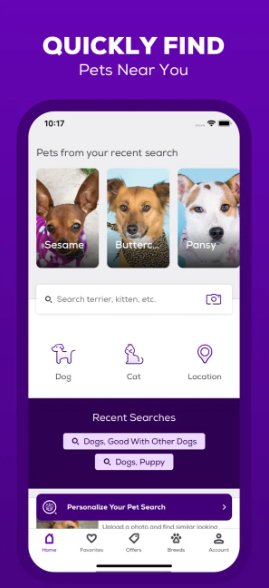
\includegraphics[width=\textwidth]{img/petfinder1.png} % Nahraďte správnou cestou
        \caption{Hlavní stránka} % Popis prvního obrázku
        \label{fig:obrazek1}
    \end{subfigure}
    \hfill
    % Druhý obrázek vpravo
    \begin{subfigure}{0.22\textwidth}
        \centering
        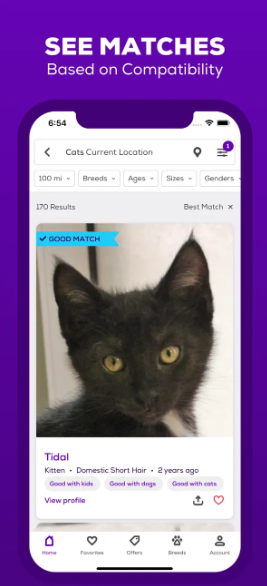
\includegraphics[width=\textwidth]{img/petfinder2.png} % Nahraďte správnou cestou
        \caption{Vybrané zvířata} % Popis druhého obrázku
        \label{fig:obrazek2}
    \end{subfigure}
    \hfill
    % Druhý obrázek vpravo
    \begin{subfigure}{0.22\textwidth}
        \centering
        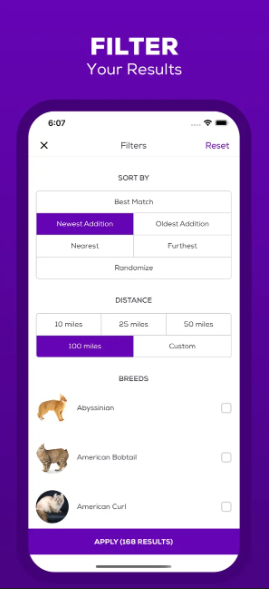
\includegraphics[width=\textwidth]{img/petfinder3.png} % Nahraďte správnou cestou
        \caption{Filtrace} % Popis druhého obrázku
        \label{fig:obrazek3}
    \end{subfigure}
    \hfill
    % Druhý obrázek vpravo
    \begin{subfigure}{0.22\textwidth}
        \centering
        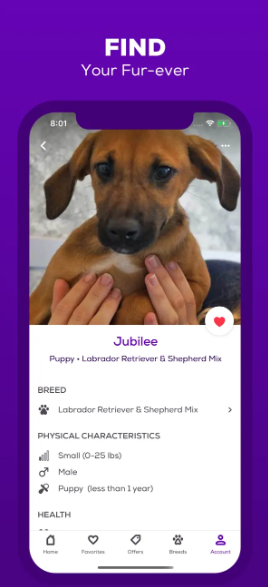
\includegraphics[width=\textwidth]{img/petfinder4.png} % Nahraďte správnou cestou
        \caption{Detail zvířete} % Popis druhého obrázku
        \label{fig:obrazek4}
    \end{subfigure}
    
    % Popisek pod celou skupinou obrázků
    \caption{Ukázky uživatelského rozhraní aplikace Petfinder} % Celkový popis
    \label{fig:obrazky-vedle-sebe}
\end{figure}


\subsection{Dog-point}

\noindent \textbf{Funkčnost}: Portál se zaměřuje na adopci psů, přičemž nabízí i možnost virtuální adopce pro psy s postižením, kteří nemohou být adoptováni. Kromě toho si zde uživatelé mohou zakoupit ručně vyráběné náramky, přívěsky a pamlsky pro své mazlíčky. Další poskytované služby zahrnují venčení, výcvik a odchyt psů. Hlavní nevýhodou je umístění útulku mimo dosah velkých měst, což může komplikovat dostupnost pro některé uživatele. Portál se specializuje výhradně na psy, což omezuje širší nabídku pro jiná domácí zvířata.\\

\noindent \textbf{Uživatelské rozhraní}: Design je přehledný a umožňuje snadnou orientaci, avšak proces adopce není plně intuitivní. Vyžaduje stažení dokumentů a jejich ruční vyplňování, což může být pro některé uživatele časově náročné a nekomfortní. Chybějící plně automatizovaný online proces snižuje celkovou uživatelskou přívětivost.\\


\noindent \textbf{Technologická řešení}: Portál funguje jako responzivní webová aplikace, která však nenabízí podporu pro nativní mobilní aplikace ani možnost integrace s jinými platformami.\\

\noindent \textbf{Regionální dostupnost}: Portál je dostupný pouze pro uživatele v České republice. Samotné umístění útulku znevýhodňuje uživatele z odlehlejších regionů, jako je například Plzeňský kraj.\\


\subsection{Puppio}

\noindent \textbf{Funkčnost}: Webový portál zaměřený na inzerci psů a koček z různých útulků. Nabízí možnost vyhledávání zvířat podle různých kritérií, jako je věk, plemeno nebo lokalita. Mezi hlavní výhody patří jednoduchost a přehlednost uživatelského rozhraní, které usnadňuje orientaci a vyhledávání zvířat. Nevýhodou je však zaměření pouze na Středočeský kraj a podle aktivity na sociálních sítích se zdá, že portál není delší dobu aktivní.\\


\noindent \textbf{Uživatelské rozhraní}: Jednoduché a přehledné rozhraní, vhodné pro základní inzerci. Portál nabízí přehledně zpracované informace o zvířatech, což může být inspirací pro návrh vlastní aplikace.\\

\noindent \textbf{Technologická řešení}: Omezeno na webové prostředí, bez podpory mobilních aplikací nebo možnosti integrace s dalšími systémy.\\

\noindent \textbf{Regionální dostupnost}: Zaměřuje se výhradně na inzeráty z oblasti Středočeského kraje.\\

\begin{figure}[h!]
    \centering
    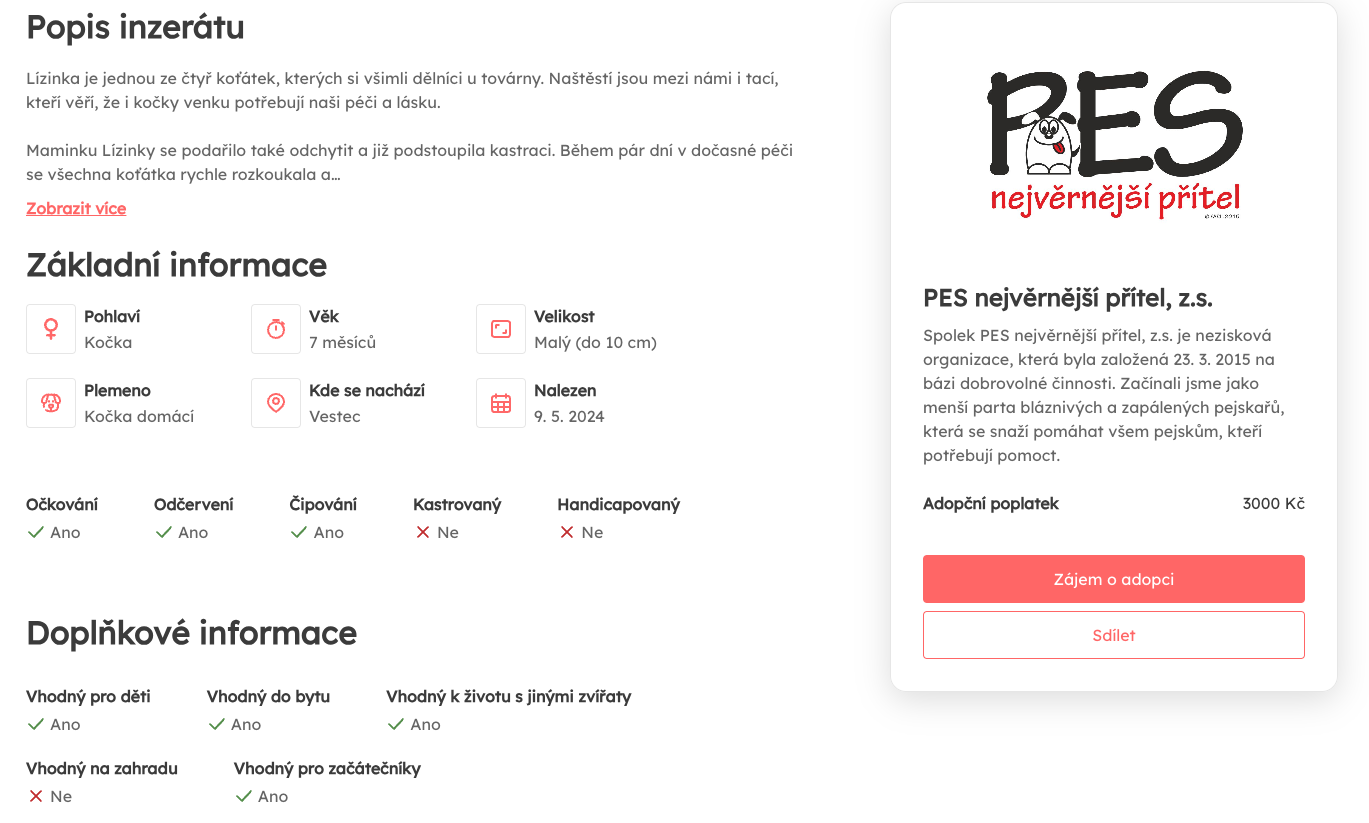
\includegraphics[width=1\textwidth]{img/puppio.png} % Cesta k obrázku
    \caption{Základní informace o zvířeti na portálu Puppio} % Popis obrázku
    \label{fig:basic-info-puppio} % Identifikátor pro odkazování na obrázky
\end{figure}


\section{Srovnání dostupných řešení}

\begin{table}[h!]
    \centering
    \begin{tabular}{|l|c|c|c|c|c|}
        \hline
        \textbf{Srovnání} & \textbf{Pesweb} & \textbf{Anidef} & \textbf{Petfinder} & \textbf{Dog-point} & \textbf{Puppio} \\ \hline
        Filtrace zvířat & Ano & Ne & Ano & Ne & Ano \\ \hline
        Široká nabídka & Omezený & Ano & Ano & Ne & Omezený \\ \hline
        Podpora mobilních zařízení & Ne & Omezený & Ano & Omezený & Omezený \\ \hline
        Regionální dostupnost & Neomezený & Omezený & Omezený & Omezený & Omezený \\ \hline
    \end{tabular}
    \caption{Srovnání dostupných řešení pro adopci a inzerci zvířat}
    \label{tab:srovnani-reseni}
\end{table}

\subsection{Shrnutí zjištění}

Tabulka \ref{tab:srovnani-reseni} nabízí přehled hlavních charakteristik analyzovaných platforem:\\

\noindent \textbf{Filtrace zvířat}: Možnost filtrace zvířat je dostupná na platformách Pesweb, Petfinder a Puppio. Z těchto řešení vyniká Petfinder, který nabízí pokročilé možnosti filtrace.\\

\noindent \textbf{Široká nabídka}: Širokou nabídku zvířat poskytují platformy Petfinder a Anidef. Ostatní platformy mají omezený nebo úzce zaměřený obsah.\\

\noindent \textbf{Podpora mobilních zařízení}: Plnou podporu mobilních zařízení nabízí pouze Petfinder. Platformy Anidef, Dog-point a Puppio mají alespoň částečnou podporu ve formě responzivního designu. Pesweb naopak mobilní zařízení nepodporuje vůbec.\\

\noindent \textbf{Regionální dostupnost}: Platforma Pesweb nabízí nejširší geografické pokrytí s dostupností po celé České republice. Naopak ostatní platformy, včetně Dog-point a Puppio, jsou geograficky omezené na specifické regiony. Petfinder je omezen na Severní Ameriku.\\

Tato analýza ukazuje, že Petfinder má pokročilé funkce a mobilní podporu, ale jeho regionální omezení značně snižuje jeho dostupnost. Pesweb má široké pokrytí a základní funkce, ale zaostává v podpoře moderních technologií. Anidef a Puppio se zaměřují na specifické regiony, přičemž Puppio nabízí moderní design, ale chybí mu širší funkcionalita.\\


\chapter{Návrh nového řešení}

Na základě provedené analýzy stávajících softwarových řešení byla identifikována řada nedostatků, které nová aplikace plánuje odstranit. Tato kapitola se zaměřuje na návrh aplikace pro inzerci a adopci domácích zvířat, přičemž cílem je vytvořit moderní, uživatelsky přívětivou a funkčně bohatou mobilní aplikaci.

\section{Sběr požadavků}

Z provedené analýzy a hodnocení uživatelských očekávání vyplývají následující požadavky na novou aplikaci:\\

\noindent \textbf{Pokročilé filtrování zvířat}: Možnost filtrování podle druhu, věku, velikosti, lokality a dalších kritérií.\\

\noindent \textbf{Uživatelská personalizace}: Doporučení zvířat na základě preferencí uživatele.\\

\noindent \textbf{Optimalizace pro mobilní zařízení}: Plně responzivní aplikace dostupná pro Android a iOS.\\

\noindent \textbf{Datová integrace s útulky}: Správa informací o zvířatech v reálném čase.\\

\noindent \textbf{Jednoduchá registrace a správa profilu}: Pro zájemce o adopci a útulky.\\

\section{Uživatelské persony a případy užití}

Aby aplikace vyhovovala potřebám cílové skupiny, byly vytvořeny uživatelské persony a scénáře použití, které reflektují nejčastější interakce uživatelů s aplikací.
\pagebreak
\subsection{Zájemce o adopci}
\begin{table}[h!]
    \centering
    \renewcommand{\arraystretch}{1.4}
    \begin{tabular}{|p{3cm}|p{10cm}|}
        \hline
        \textbf{Popis} & Uživatel hledající vhodné zvíře k adopci. \\ \hline
        \textbf{Cíl} & Najít zvíře dle preferencí, prohlédnout informace a dokončit adopční proces. \\ \hline
        \textbf{Scénář použití} &
        \begin{itemize}
            \item Registrace do aplikace a vyplnění profilu.
            \item Použije filtry (věk, plemeno, lokalita) k vyhledání zvířat.
            \item Prohlédne si detailní informace o vybraném zvířeti.
            \item Kontaktuje útulek s žádostí o adopci.
        \end{itemize} \\ \hline
    \end{tabular}
    \caption{Persona: Zájemce o adopci.}
    \label{tab:persona_adopter}
\end{table}

\subsection{Zaměstnanec útulku}
\begin{table}[h!]
    \centering
    \renewcommand{\arraystretch}{1.4}
    \begin{tabular}{|p{3cm}|p{10cm}|}
        \hline
        \textbf{Popis} & Pracovník útulku spravující nabídku zvířat k adopci. \\ \hline
        \textbf{Cíl} & Přidat nová zvířata do systému a sledovat stav adopčních žádostí. \\ \hline
        \textbf{Scénář použití} &
        \begin{itemize}
            \item Registruje útulek do aplikace a nahraje nové zvíře s fotografiemi a podrobnými informacemi.
            \item Sleduje adopční žádosti a komunikuje mimo aplikaci s uživateli.
        \end{itemize} \\ \hline
    \end{tabular}
    \caption{Persona: Zaměstnanec útulku.}
    \label{tab:persona_shelter_worker}
\end{table}

\newpage

\section{Návrh aplikace}

\subsection{Registrace a přihlášení}

Proces registrace a přihlášení je navržen tak, aby byl intuitivní, bezpečný a přizpůsobený dvěma typům uživatelů: běžnému uživateli (zájemci o adopci) a zástupci útulku.\\

\noindent \textbf{Registrace běžného uživatele}: Nový uživatel zadává při registraci následující základní údaje:
\begin{itemize}[leftmargin=2em]
    \item jméno a příjmení,
    \item e-mailovou adresu (sloužící zároveň jako přihlašovací jméno),
    \item datum narození,
    \item heslo pro přihlášení.
\end{itemize}

\noindent \textbf{Registrace útulku}: V případě, že se registruje útulek, je po vytvoření základního účtu (stejně jako u běžného uživatele) zobrazen navazující formulář pro doplnění detailních informací o organizaci. Tyto údaje zahrnují:
\begin{itemize}[leftmargin=2em]
    \item název útulku,
    \item registrační číslo Státní veterinární správy (pro ověření pravosti subjektu),
    \item ulici a číslo popisné,
    \item město,
    \item rok vzniku organizace,
    \item počet uskutečněných adopcí za poslední rok,
    \item telefonní kontakt,
    \item popis útulku a jeho činnosti,
    \item možnost nahrát až 6 fotografií zařízení.
\end{itemize}

\noindent Tyto informace jsou následně uloženy do příslušné kolekce v databázové vrstvě aplikace, přičemž každému útulku je přiřazen samostatný profil.\\

\noindent \textbf{Přihlášení}: Uživatelé se do systému přihlašují pomocí e-mailové adresy a hesla. 


\subsection{Hlavní obrazovka aplikace}

Hlavní obrazovka aplikace (viz obrázek \ref{fig:main-stranka}) slouží jako výchozí bod pro uživatele a poskytuje přehledné rozhraní pro navigaci a interakci s klíčovými funkcemi aplikace. Její návrh se zaměřuje na intuitivní ovládání a rychlý přístup k potřebným informacím.\\

\noindent \textbf{Spodní navigační panel}: Obsahuje ikony pro rychlý přístup k hlavním sekcím aplikace, jako jsou \textit{Domů}, \textit{Vyhledávání}, \textit{Oblíbené} a \textit{Profil}. Navigace je umístěna ve spodní části obrazovky pro snadnou dostupnost při ovládání jednou rukou.\\

\noindent \textbf{Vyhledávací panel}: Nachází se v horní části obrazovky a umožňuje vyhledávání zvířat podle různých kritérií. Mezi dostupné filtry patří:
\begin{itemize}
    \item Druh zvířete (pes, kočka, jiná zvířata),
    \item Věk,
    \item Plemeno,
    \item Lokalita.
\end{itemize}

\noindent \textbf{Výsledky vyhledávání}: Zobrazeny ve formě přehledných karet, které obsahují:

\begin{itemize}
    \item Fotografie zvířete,
    \item Základní informace (jméno, věk, lokalita).
\end{itemize}

\noindent Kliknutím na kartu se uživateli zobrazí detailní informace o zvířeti, včetně dalších fotografií, podrobného popisu a možnosti kontaktovat útulek.\\

\noindent \textbf{Zájem o adopci}: Uživatel může vyjádřit zájem o zvíře stisknutím tlačítka s ikonou srdce nebo přetažením karty doprava.\\

\noindent \textbf{Odmítnutí zvířete}: Přetažením karty doleva může uživatel zvíře odmítnout a pokračovat ve vyhledávání.\\

\noindent \textbf{Kontaktování útulku}: V případě výrazného zájmu má uživatel možnost stisknout tlačítko s ikonou vlaštovky a přímo kontaktovat útulek.\\

\begin{figure}[h!]
    \centering
    \begin{subfigure}{0.3\textwidth}
        \centering
        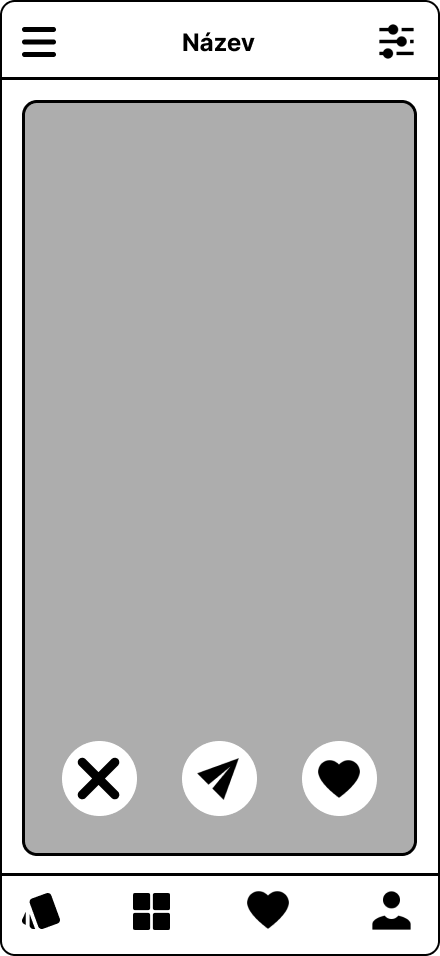
\includegraphics[width=\textwidth]{img-bp/Main.png} 
        \caption{Wireframe}
        \label{fig:wireframe-main}
    \end{subfigure}
    \hfill
    \begin{subfigure}{0.3\textwidth}
        \centering
        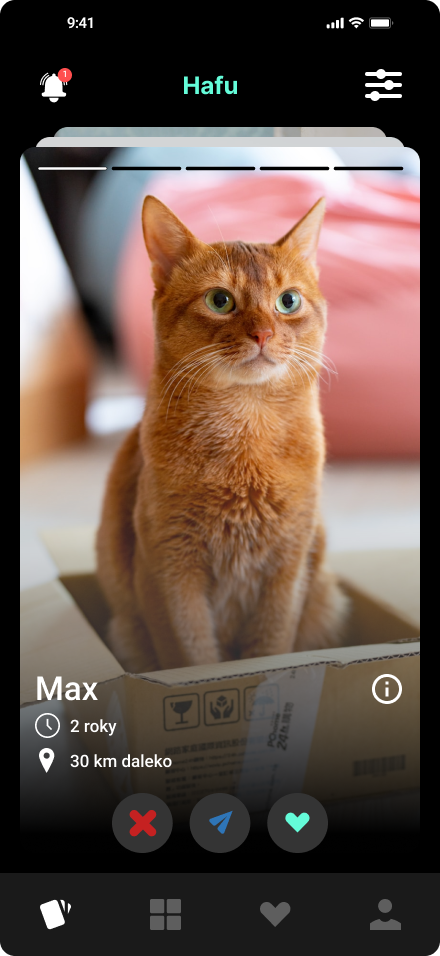
\includegraphics[width=\textwidth]{img-bp/Main-g.png} 
        \caption{UI návrh}
        \label{fig:ui-main}
    \end{subfigure}
    \hfill
    \begin{subfigure}{0.3\textwidth}
        \centering
        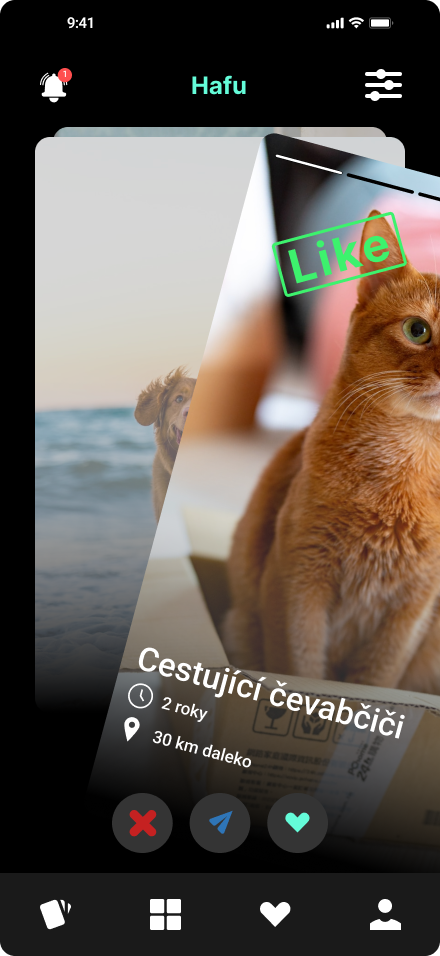
\includegraphics[width=\textwidth]{img-bp/Main-like-g.png}
        \caption{UI nárvh reakce na like}
        \label{fig:main-stranka}
    \end{subfigure}
    \hfill
    \caption{Ukázky uživatelského rozhraní hlavní obrazovky}
    \label{fig:obrazky-vedle-sebe}
\end{figure}


\noindent Hlavní obrazovka aplikace je navržena s důrazem na jednoduchost, přehlednost a efektivní ovládání, aby co nejvíce usnadnila uživatelům proces vyhledávání a adopce zvířat.

\subsection{Vyhledávací obrazovka}

\noindent Vyhledávací obrazovka (viz obrázek \ref{fig:explore-stranka}) je navržena tak, aby uživatelům umožnila efektivní procházení nabídky zvířat a přizpůsobení výsledků dle konkrétních preferencí. Oproti hlavní obrazovce nabízí stejné možnosti filtrování, ale podrobnější kategorizaci obsahu.\\

\noindent \textbf{Horní panel}: Vrchní část obrazovky obsahuje dvě důležité komponenty:

\begin{itemize}[leftmargin=2em]
    \item \textbf{Vyhledávací pole} – umožňuje vyhledávat zvířata dle různých kritérií. Mezi dostupné filtry patří:
    \begin{itemize}
        \item druh zvířete (pes, kočka, jiná zvířata),
        \item věk,
        \item plemeno,
        \item lokalita.
    \end{itemize}
    
    \item \textbf{Tlačítko menu} – umístěné na levé straně horní lišty, slouží k vyvolání postranního navigačního panelu (drawer) s doplňkovými funkcemi.
\end{itemize}

\noindent \textbf{Tělo obrazovky}: Hlavní část zobrazuje zvířata ve formě dlaždic uspořádaných do mřížky. Každá dlaždice obsahuje náhledovou fotografii a základní informace o daném zvířeti. Zobrazují se všechna dostupná zvířata v aplikaci nebo pouze ta, která odpovídají zadaným filtrům. Uživatel se může jednoduše posouvat ze shora dolů, nebo naopak a vybírat ze široké nabídky zvířat.\\

\noindent \textbf{Detail zvířete}: Kliknutím na konkrétní dlaždici se otevře obrazovka s detailními informacemi. Z této obrazovky může uživatel:
\begin{itemize}
    \item Přidat zvíře do seznamu oblíbených,
    \item Kontaktovat příslušný útulek pomocí tlačítka.
\end{itemize}

\noindent \textbf{Spodní navigační panel}: Stejně jako na ostatních obrazovkách, i zde je ve spodní části obrazovky přítomen tabulátorový panel s hlavními sekcemi aplikace (Domů, Procházet, Oblíbené, Můj profil), který zajišťuje rychlou orientaci a návrat do klíčových částí rozhraní.

Vyhledávací obrazovka je koncipována s důrazem na přehlednost, uživatelskou přívětivost a rychlou navigaci mezi kategoriemi, filtry a detaily jednotlivých zvířat. Umožňuje tak uživateli snadno najít vhodného kandidáta k adopci.

\begin{figure}[h!]
    \centering
    \begin{subfigure}{0.3\textwidth}
        \centering
        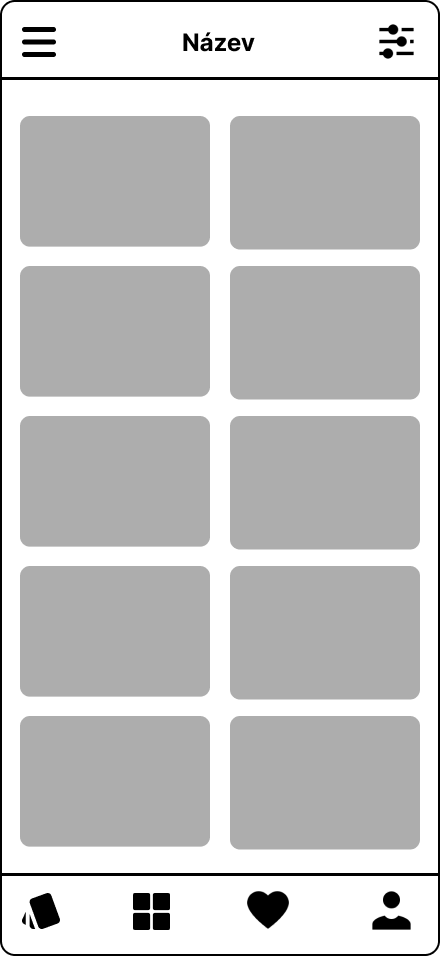
\includegraphics[width=\textwidth]{img-bp/Explore.png} 
        \caption{Wireframe}
        \label{fig:wireframe-explore}
    \end{subfigure}
    \hspace{0.05\textwidth}
    \begin{subfigure}{0.3\textwidth}
        \centering
        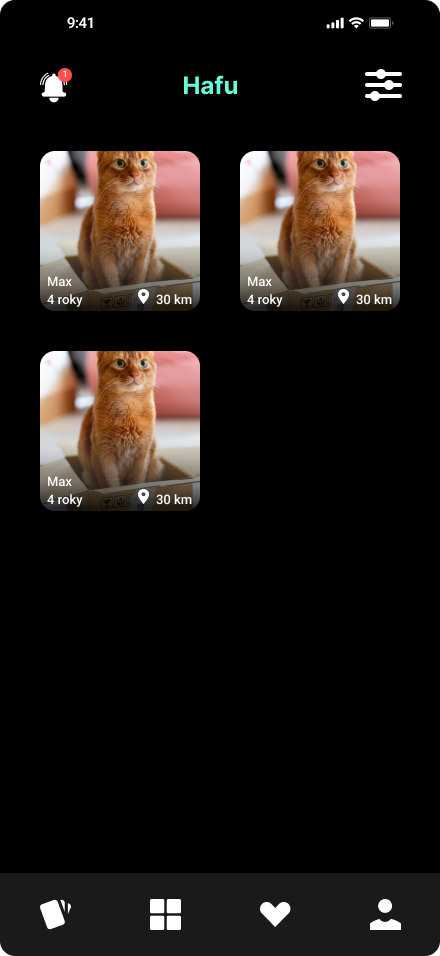
\includegraphics[width=\textwidth]{img-bp/Explore-g.png} 
        \caption{UI návrh}
        \label{fig:ui-explore}
    \end{subfigure}
    \caption{Ukázky uživatelského rozhraní vyhledáváci obrazovky}
    \label{fig:explore-stranka}
\end{figure}

\subsection{Obrazovka Oblíbené}

Obrazovka \textbf{Oblíbené} (viz obrázek \ref{fig:like-stranka}) slouží k přehlednému zobrazení všech zvířat, o která uživatel v minulosti projevil zájem – buď prostřednictvím gesta typu \textit{like} v rozhraní hlavní obrazovky, nebo stisknutím tlačítka se symbolem srdce na detailu zvířete.\\

\begin{figure}[h!]
    \centering
    \begin{subfigure}{0.3\textwidth}
        \centering
        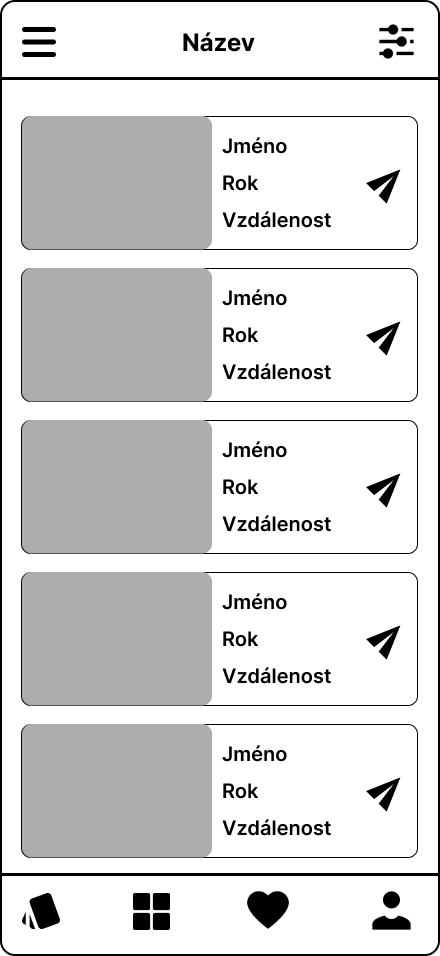
\includegraphics[width=\textwidth]{img-bp/Like.png} 
        \caption{Wireframe}
        \label{fig:wireframe-like}
    \end{subfigure}
    \hspace{0.05\textwidth}
    \begin{subfigure}{0.3\textwidth}
        \centering
        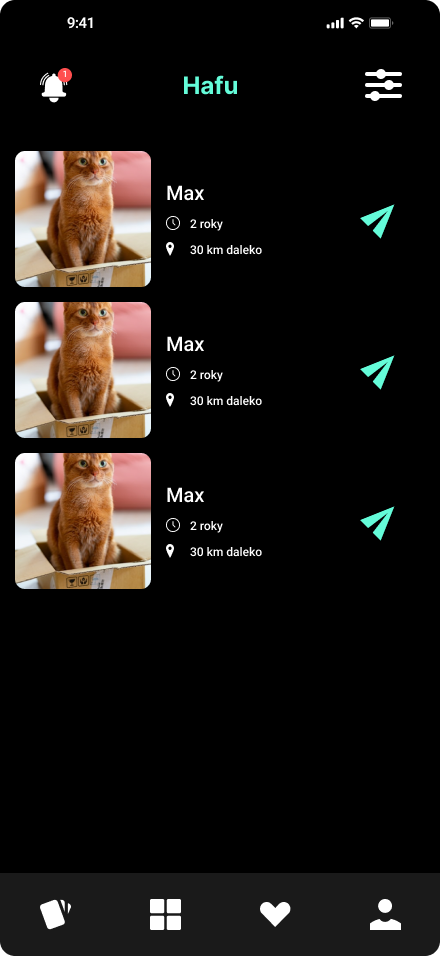
\includegraphics[width=\textwidth]{img-bp/Like-g.png} 
        \caption{UI návrh}
        \label{fig:ui-like}
    \end{subfigure}
    \caption{Ukázky uživatelského rozhraní obrazovky oblíbené}
    \label{fig:like-stranka}
\end{figure}

\noindent \textbf{Tělo obrazovky}: Všechna označená zvířata jsou prezentována ve formě svisle řazených dlaždic, přičemž každá dlaždice obsahuje:
\begin{itemize}[leftmargin=2em]
    \item náhledovou fotografii zvířete,
    \item základní informace jako jméno, přibližný věk a vzdálenost od uživatele,
    \item tlačítko pro rychlý přechod na kontaktní formulář útulku.
\end{itemize}

\noindent \textbf{Interaktivita dlaždic}: Kliknutím na samotnou fotografii zvířete, případně na oblast mimo tlačítko pro kontakt, je uživatel přesměrován na detailní obrazovku daného zvířete. Tím je zachována možnost rychlého náhledu i hlubší interakce.\\

\noindent \textbf{Tlačítko kontaktu}: Každá dlaždice obsahuje viditelně umístěné tlačítko pro kontaktování příslušného útulku. Po jeho stisknutí se uživatel přesměruje přímo na formulář, kde může vyjádřit zájem o adopci, případně položit doplňující otázky.\\

\noindent \textbf{Navigační prvky}: Spodní navigační panel zůstává zachován v identické podobě jako na ostatních hlavních obrazovkách aplikace, což zajišťuje konzistentní a snadnou orientaci v rozhraní.\\

\noindent Tato obrazovka poskytuje uživateli pohodlný přístup k výběru kandidátů na adopci, které si v průběhu používání aplikace označil jako oblíbené, a umožňuje snadno navázat kontakt s útulky.



\subsection{Obrazovka profilu}

Obrazovka profilu (viz obrázek \ref{fig:profile-stranka}) slouží uživateli jako centrální místo pro správu jeho osobních údajů a nastavení aplikace. Uživatel zde může provádět následující akce:\\

\begin{figure}[h!]
    \centering
    \begin{subfigure}{0.3\textwidth}
        \centering
        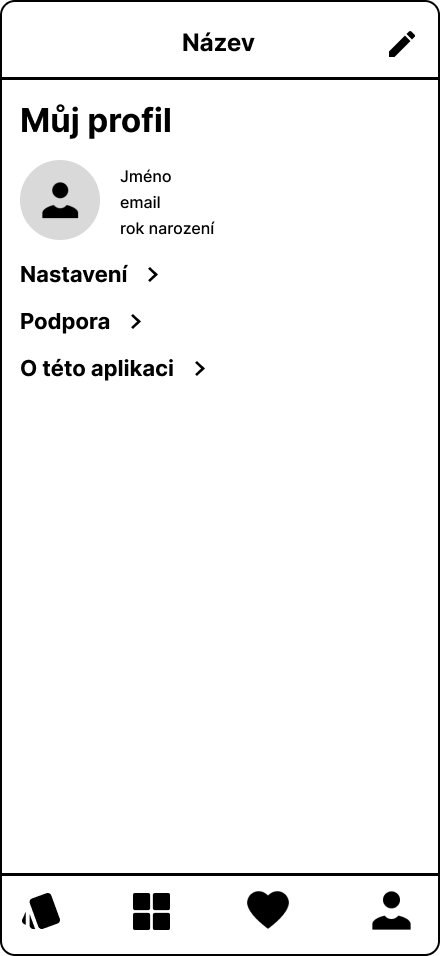
\includegraphics[width=\textwidth]{img-bp/Account.png} 
        \caption{Wireframe}
        \label{fig:wireframe-profile}
    \end{subfigure}
    \hspace{0.05\textwidth}
    \begin{subfigure}{0.3\textwidth}
        \centering
        
\includegraphics[width=\textwidth]{img-bp/Account-g.png} 
        \caption{UI návrh}
        \label{fig:ui-profile}
    \end{subfigure}
    \caption{Ukázky uživatelského rozhraní obrazovky profilu}
    \label{fig:profile-stranka}
\end{figure}

\noindent \textbf{Úprava osobních informací}: Uživatel má možnost změnit své základní údaje, jako je jméno, e-mail nebo profilová fotografie.\\

\noindent \textbf{Přístup k nastavení}: Tlačítko pro přechod na stránku nastavení, kde lze přizpůsobit funkce aplikace (např. notifikace, jazyk rozhraní).\\

\noindent \textbf{Podpora a informace o aplikaci}: Možnost přesměrování na sekci technické podpory nebo zobrazení informací o aplikaci, včetně verzí a kontaktů na vývojářský tým.\\

\noindent Obrazovka profilu je navržena tak, aby uživatelům poskytla jednoduchý a přehledný přístup k osobním nastavením a informacím o aplikaci.

\subsection{Postranní menu a funkce pro útulky}

Uživatel typu \textit{útulek} má po přihlášení do aplikace rozšířený přístup k administračním funkcím, které jsou dostupné prostřednictvím postranního navigačního panelu. Tento panel je vyvolatelný z horního baru pomocí ikony menu (tzv. hamburger menu).\\

\noindent \textbf{Správa zvířat}: Jednou z klíčových funkcí dostupných v postranním menu je přístup k obrazovce \textit{Správa zvířat}, která umožňuje:
\begin{itemize}[leftmargin=2em]
    \item přidávat nová zvířata do systému prostřednictvím formuláře s podrobnými informacemi,
    \item upravovat stávající inzeráty (např. doplnění údajů, aktualizace stavu),
    \item odstraňovat záznamy zvířat, která již nejsou aktuální,
    \item dočasně skrýt zvířata z veřejné nabídky v případě, že o ně někdo projevil zájem nebo čekají na schválení adopce.
\end{itemize}

\noindent \textbf{Profil útulku}: Druhou důležitou sekcí v postranním panelu je \textit{Profil útulku}. Tato obrazovka slouží k revizi a editaci údajů o organizaci, které byly zadány při registraci. Útulek zde může:
\begin{itemize}[leftmargin=2em]
    \item zkontrolovat správnost zadaných údajů,
    \item upravit vybrané informace (např. kontaktní údaje, popis zařízení, fotografie),
    \item odstranit zastaralé nebo chybné údaje.
\end{itemize}

\noindent Tato struktura zajišťuje, že útulky mají nad svými daty plnou kontrolu, a zároveň mohou v reálném čase spravovat aktuální nabídku zvířat dostupných k adopci.

\subsection{Přidání nového zvířete útulkem}

Funkce pro přidání nového zvířete do systému je dostupná uživatelům typu \textit{útulek} v sekci \textit{Správa zvířat}. Proces probíhá prostřednictvím intuitivního formuláře, který pokrývá všechny relevantní informace potřebné pro zveřejnění zvířete k adopci.

\noindent \textbf{Formulář pro přidání zvířete} obsahuje následující položky:
\begin{itemize}[leftmargin=2em]
    \item \textbf{Typ zvířete} – uživatel zvolí druh zvířete (např. pes, kočka, jiné),
    \item \textbf{Jméno} zvířete,
    \item \textbf{Interní identifikační číslo} – slouží výhradně pro evidenci zvířat v rámci útulku,
    \item \textbf{Pohlaví} – výběr mezi samcem a samicí,
    \item \textbf{Přibližné datum narození} – zadává se ve formátu měsíc a rok,
    \item \textbf{Velikost} – vybírá se z předdefinované nabídky (např. malý, střední, velký),
    \item \textbf{Datum nalezení nebo přijetí do útulku},
    \item \textbf{Plemeno} – vybírá se z katalogu dostupných plemen,
    \item \textbf{Kříženec} – pokud je zvíře křížené, aktivuje se možnost výběru až tří plemen, ze kterých je složeno,
    \item \textbf{Zdravotní stav} – série zaškrtávacích polí pro:
    \begin{itemize}
        \item očkované (ano/ne),
        \item odčervené (ano/ne),
        \item čipované (ano/ne),
        \item kastrované (ano/ne),
        \item handicapované (ano/ne) – v případě zaškrtnutí se zobrazí doplňkové pole pro popis handicapu.
    \end{itemize}
    \item \textbf{Popis zvířete} – volné textové pole pro zadání informací o povaze, historii či specifických potřebách,
    \item \textbf{Adopční poplatek} – vyjádřený v Kč, 
    \item \textbf{Fotografie} – možnost nahrát až 6 snímků daného zvířete.
\end{itemize}

Formulář je navržen tak, aby podporoval validaci vstupů a poskytoval útulku potřebnou míru kontroly nad zveřejněnými informacemi. Po odeslání formuláře je nový záznam okamžitě uložen do databáze a zveřejněn v katalogu zvířat dostupných k adopci.


\section{Výběr technologií a zdůvodnění volby}

\subsection{Použitá technologie pro vývoj aplikace}

Pro vývoj mobilní aplikace bude použita technologie \product{React Native} s frameworkem \product{Expo}. \product{React Native} umožňuje tvorbu multiplatformních aplikací pro \product{Android} i \product{iOS} s využitím jednoho kódu, přičemž výsledná aplikace dosahuje nativního výkonu díky využití nativních komponent. Technologie \product{React Native} je založena na knihovně \product{React}, což usnadňuje tvorbu modulárních a responzivních uživatelských rozhraní.

Framework \product{Expo} rozšiřuje funkcionalitu \product{React Native} o širokou škálu nástrojů a modulů, jako jsou navigace, přístup k senzorům a \product{GPS} nebo snadná integrace nativních funkcí. \product{Expo} rovněž umožňuje rychlý start projektu a jednoduché testování aplikace, čímž významně zefektivňuje celý proces vývoje. Tato kombinace poskytuje moderní, flexibilní a škálovatelné řešení pro vývoj mobilní aplikace \cite{reactnative}.



\subsection{Použitá technologie pro backend}

Pro realizaci backendové části aplikace je zvolena open-source platforma \product{Appwrite}, která poskytuje komplexní infrastrukturu pro vývoj moderních webových a mobilních aplikací. \product{Appwrite} nabízí vestavěnou podporu pro autentizaci uživatelů, správu databáze, práci s úložištěm souborů, plánování úloh a funkce v reálném čase (např. notifikace nebo změnové události).

Databázová vrstva je v \product{Appwrite} založena na systému kolekcí a dokumentů, přičemž každá kolekce má definované schéma a přístupová pravidla. Platforma umožňuje podrobné řízení oprávnění až na úrovni jednotlivých dokumentů díky flexibilním pravidlům přístupu, která lze definovat pro čtení, zápis, vytvoření nebo smazání dat.

\product{Appwrite} rovněž poskytuje bezpečnostní funkce jako je správa uživatelských relací, dvoufaktorová autentizace, ochrana proti útokům typu brute-force a auditní logy. Vývojářům je k dispozici klientské SDK pro různé jazyky a platformy včetně \product{JavaScript}, \product{React Native}, \product{Flutter} či \product{Node.js}, což usnadňuje integraci s frontendovou částí aplikace.

Díky možnosti samostatného hostování pomocí \product{Docker} kontejnerů je \product{Appwrite} vhodný i pro projekty, které vyžadují provoz na vlastním serveru a vyšší míru kontroly nad daty. Tato technologie byla zvolena pro svou modularitu, otevřenost, přehlednou dokumentaci a podporu rychlého vývoje moderních aplikací \cite{appwrite}.




\section{Shrnutí návrhu}

Tato kapitola představila návrh mobilní aplikace zaměřené na inzerci a adopci domácích zvířat, která reaguje na identifikované nedostatky v současných softwarových řešeních. Hlavním cílem návrhu je vytvoření moderní, funkčně bohaté a uživatelsky přívětivé aplikace.

Nová aplikace je navržena s ohledem na klíčové funkční požadavky, jako jsou pokročilé filtrování zvířat, personalizovaná doporučení, optimalizace pro mobilní zařízení, snadná registrace uživatelů i útulků a správa dat v reálném čase. V rámci návrhu byly definovány uživatelské persony, které reprezentují hlavní cílové skupiny aplikace – zájemce o adopci a zaměstnance útulků. Tyto persony byly doplněny scénáři použití, které ilustrují nejčastější interakce uživatelů s aplikací.

Aplikace obsahuje několik klíčových obrazovek, mezi které patří hlavní obrazovka, vyhledávací obrazovka, sekce oblíbených a profilová obrazovka. Každá obrazovka byla detailně popsána a návrh byl podpořen ukázkami uživatelského rozhraní.

Pro vývoj aplikace byla zvolena technologie \product{React Native} společně s frameworkem \product{Expo}. Tato kombinace umožňuje efektivní vývoj multiplatformních aplikací pro \product{Android} a \product{iOS} s flexibilním uživatelským rozhraním. Backend aplikace je postaven na technologii \product{Appwrite}, která poskytuje robustní řešení pro správu databáze, autentizaci, úložiště a synchronizaci dat v reálném čase. Tyto technologie byly vybrány pro jejich škálovatelnost, jednoduchou implementaci a podporu moderních vývojářských procesů.

Návrh aplikace a výběr použitých technologií tvoří základ pro realizaci komplexního a uživatelsky přívětivého řešení, které bude přínosné jak pro zájemce o adopci, tak pro útulky nabízející zvířata k adopci.




\chapter{Návrh aplikace}

Tato kapitola se zaměřuje na podrobný návrh mobilní aplikace pro inzerci a adopci domácích zvířat. Nejprve je představena celková architektura systému a zvolené technologie. Dále je popsána struktura, tok aplikace z pohledu uživatele a hlavních obrazovek. Následuje výčet klíčových funkcí aplikace a návrh datového modelu spolu s API rozhraním pro komunikaci mezi mobilní aplikací a backendem.

\section{Architektura a zvolené technologie}

Navrhovaná aplikace je koncipována jako klasický klient--server systém. Klientskou část představuje mobilní aplikace vyvinutá pomocí multiplatformního frameworku \product{React Native}, konkrétně s využitím nástroje \product{Expo}, který zjednodušuje vývoj a nasazení aplikací na platformách \product{Android} i \product{iOS}.

Serverová část je realizována pomocí open-source backendové platformy \product{Appwrite}, jež poskytuje komplexní sadu služeb jako autentizaci uživatelů, správu databáze a úložiště souborů. Původně byl pro backend zvažován systém \product{Supabase}. Avšak s ohledem na požadavek samostatného hostování a vyšší flexibilitu při škálování systému byl zvolen \product{Appwrite} jako vhodnější alternativa.

\product{Appwrite} byl od začátku navržen s důrazem na snadnou instalaci a provoz na vlastním serveru. Lze jej spustit na jakémkoli zařízení podporujícím \product{Docker}, čímž se výrazně zjednodušuje nasazení i správa. Navíc poskytuje stejné funkce jako jeho cloudová varianta. Minimální hardwarové požadavky pro běh \product{Appwrite} jsou 4~GB RAM, což svědčí o nízké náročnosti na infrastrukturu\cite{appwrite-selfhosting}.

Interně využívá platforma \product{Appwrite} relační databázový systém \product{MariaDB}, přičemž architektura systému je navržena tak, aby v budoucnu podporovala i další databázové adaptéry, jako jsou \product{MySQL} nebo \product{MongoDB}. Nad databázovou vrstvou \product{Appwrite} vystavuje vlastní abstraktní rozhraní ve stylu \product{NoSQL} – aplikace pracuje s kolekcemi a dokumenty, přičemž každá kolekce obsahuje strukturované záznamy s definovanými atributy, typy a validací vstupů.

Každý dokument v kolekci dodržuje předem určené schéma, které může obsahovat atributy různých typů (např. řetězec, celé číslo, boolean, datum a čas, e-mail, URL či relaci na jinou kolekci). \product{Appwrite} zároveň podporuje definici indexů pro urychlení dotazů, včetně indexů typu \texttt{unique}, \texttt{fulltext} a \texttt{key}, čímž umožňuje efektivní vyhledávání a zamezuje duplicitám v uložených datech  \cite{appwrite-collections}.

Platforma také nabízí podporu více než deseti programovacích jazyků pro vývoj tzv. serverless funkcí. V kombinaci s nízkými systémovými požadavky a jednoduchým nasazením představuje \product{Appwrite} robustní řešení pro samostatné hostování backendové infrastruktury.



\subsection{React Native a Expo}

\subsubsection*{React Native}

Pro vývoj klientské části aplikace bylo zvoleno prostředí \product{React Native} ve spojení s platformou \product{Expo}. \product{React Native} je framework vyvinutý společností \product{Meta} (dříve \product{Facebook}), který umožňuje tvorbu skutečně nativních mobilních aplikací s využitím jazyka \product{JavaScript} a knihovny \product{React}. Výsledná aplikace není hybridní ani webová, ale plnohodnotná nativní aplikace, využívající stejné základní uživatelské komponenty jako aplikace psané v jazycích \product{Swift} pro \product{iOS} nebo \product{Kotlin}/\product{Java} pro \product{Android}. Rozdíl spočívá v tom, že tyto komponenty jsou definovány prostřednictvím JavaScriptového rozhraní Reactu \cite{reactnative}.


\subsubsection*{Expo a EAS}

\textbf{\product{Expo}} je open-source platforma nad frameworkem \product{React Native}, která usnadňuje vývoj, testování a nasazení multiplatformních mobilních aplikací. Umožňuje vytvářet nativní aplikace pomocí jazyka \product{JavaScript} a knihovny \product{React}, a to současně pro platformy \product{Android}, \product{iOS} i web. \product{Expo} poskytuje jednotné vývojové prostředí, bohaté SDK a nástroje jako \product{Expo Go} pro okamžité testování aplikací na fyzických zařízeních bez nutnosti jejich sestavování.

Klíčovým prvkem platformy je \textbf{EAS (Expo Application Services)}, která rozšiřuje možnosti vývojového cyklu o nástroje pro buildování, distribuci, aktualizace a monitoring aplikací. Díky EAS lze například:

\begin{itemize}
    \item vytvářet a odesílat produkční sestavení aplikací do \product{App Store} nebo \product{Google Play},
    \item publikovat aktualizace aplikace \textit{over-the-air} bez nutnosti opětovného schvalování,
    \item spouštět end-to-end testy, automatizovat release procesy,
    \item sledovat stav nasazení přes přehledné webové dashboardy.
\end{itemize}

Vývojáři mohou využívat Expo CLI, webové nástroje (např. Snack) a podporu pro pokročilé workflow, včetně podpory TypeScriptu, file-based routingu či integrace s \product{GitHub Actions}. \product{Expo} je široce používané ve vývoji mobilních aplikací – dle statistik používá tuto technologii více než polovina všech projektů postavených na \product{React Native}.

Díky otevřenosti, snadnému použití, aktivní komunitě a možnosti škálování od prototypování po produkční aplikace je \product{Expo} preferovaným nástrojem při vývoji moderních mobilních řešení \cite{expo2025}.


Použití \product{Expo} v tomto projektu přineslo několik výhod:
\begin{itemize}
    \item zjednodušené prostředí pro rychlé prototypování,
    \item podpora funkce \texttt{Hot Reload}, která umožňuje okamžité zobrazení změn v běžící aplikaci,
    \item jednotný vývojový proces pro platformy \product{Android} a \product{iOS}.
\end{itemize}

Projekt byl inicializován pomocí nástroje \texttt{create-expo-app} a je implementován v jazyce \product{TypeScript}. Navigace v aplikaci je řešena pomocí systému \texttt{Expo Router}, který využívá souborovou strukturu pro definici obrazovek. Tento přístup přispívá k přehledné organizaci kódu a snadnější správě jednotlivých částí aplikace.



\subsection{Appwrite – autentizace, databáze a úložiště}

Serverová část systému je postavena na open-source platformě \product{Appwrite}, která poskytuje klíčové backendové služby nezbytné pro chod aplikace. Mezi hlavní funkcionality \product{Appwrite} patří správa uživatelů (autentizace), databázová vrstva pro uchovávání aplikačních dat a úložiště pro správu souborů (např. fotografií zvířat a útulků) \cite{appwrite}.

\subsubsection*{Autentizace uživatelů.} 
Platforma \product{Appwrite} poskytuje robustní a bezpečný systém pro správu uživatelské autentizace. Podporuje více metod ověření, včetně klasického přihlášení pomocí e-mailové adresy a hesla, přihlášení přes OAuth2 poskytovatele (např. \product{Google}, \product{Facebook}, \product{GitHub}), magických odkazů (Magic URL), jednorázových hesel zasílaných e-mailem (Email OTP) a také možnost anonymního přístupu.

V rámci této aplikace byla implementována autentizace prostřednictvím e-mailu a hesla. Při registraci jsou uživatelská data uložena v databázi \product{Appwrite}, přičemž hesla jsou chráněna pomocí moderního hashovacího algoritmu \product{Argon2}. Tento algoritmus je doplněn o tzv. \textit{salting}, paměťovou náročnost a nastavitelné pracovní faktory, což zajišťuje vysokou míru bezpečnosti uchovávaných hesel. \product{Appwrite} zároveň implementuje bezpečnostní funkce, které brání použití slabých nebo snadno uhodnutelných hesel – např. zákaz použití běžně se vyskytujících hesel (tzv. \textit{password dictionary}), kontrola historie hesel a možnost blokace hesel obsahujících osobní údaje uživatele (např. jméno, e-mail).

Každý úspěšně přihlášený uživatel obdrží autentizační token a je mu vytvořena relace, která je na různých platformách ukládána (např. v \texttt{SharedPreferences} pro \product{Android} nebo \texttt{UserDefaults} pro \product{iOS}). \product{Appwrite} SDK zajišťuje správu těchto relací automaticky, takže uživatel není nucen se znovu přihlašovat při každém spuštění aplikace. Zároveň lze nastavit limit počtu aktivních relací na jednoho uživatele – výchozí hodnota je 10 relací, maximální limit je 100. Při jeho překročení je nejstarší relace automaticky ukončena.

Pro zajištění ochrany osobních údajů \product{Appwrite} podporuje granularitu oprávnění na úrovni jednotlivých zdrojů (kolekce, dokumenty, soubory apod.) prostřednictvím tzv. \textit{permissions modelu}, který je přímo provázán s uživatelskými relacemi. Přístup ke konkrétním datům tedy není závislý pouze na autentizaci, ale rovněž na explicitně udělených oprávněních.

Dále je možné aktivovat funkce jako upozornění na nové přihlášení (tzv. \textit{session alerts}), správu členství s ochranou osobních údajů (\textit{membership privacy}) nebo použití testovacích (mock) telefonních čísel pro ověřování pomocí SMS během vývoje.

Správa uživatelských účtů a relací v této aplikaci je realizována prostřednictvím oficiálního SDK \product{Appwrite} pro \product{React Native}, které komunikuje se serverem pomocí REST API. Tato integrace umožňuje bezpečné ověřování uživatelů, správu relací a zabezpečený přístup ke všem službám aplikace \cite{appwrite-auth}.




\subsubsection*{Databáze} 

Platforma \product{Appwrite} poskytuje moderní a flexibilní databázovou vrstvu, která umožňuje správu strukturovaných dat prostřednictvím tzv. \textit{kolekcí dokumentů}. Každá databáze může obsahovat více kolekcí, přičemž každá kolekce slouží jako kontejner pro dokumenty se stejnou strukturou. Struktura je definována pomocí atributů (např. \texttt{string}, \texttt{integer}, \texttt{boolean}, \texttt{datetime}, \texttt{email}, \texttt{enum} apod.), které \product{Appwrite} validuje při vytváření a aktualizaci dokumentů.

V rámci tohoto projektu byla databázová vrstva navržena pomocí několika kolekcí reprezentujících klíčové doménové entity jako \textit{uživatelé}, \textit{zvířata}, \textit{útulky}, případně pomocné kolekce pro interakce mezi uživateli a zvířaty (např. označení jako oblíbené). Každá kolekce má definováno vlastní schéma a přístupová pravidla, která určují, kdo může data číst, zapisovat, aktualizovat nebo mazat. Oprávnění lze nastavovat na úrovni jednotlivých dokumentů, kolekcí, nebo globálně — a to pro konkrétního uživatele, tým, roli nebo veřejnost.

Databázové API \product{Appwrite} umožňuje standardní CRUD operace (\texttt{createDocument}, \texttt{getDocument}, \texttt{updateDocument}, \texttt{deleteDocument}) a podporuje dotazování pomocí pole parametrů typu \texttt{query}, včetně filtrování, řazení a stránkování výsledků. Na straně klienta (v tomto případě \product{React Native}) se používá klientská knihovna \product{Appwrite SDK}, která umožňuje přímou práci s databází prostřednictvím \product{REST API}.

Tato architektura umožňuje snadné rozšiřování datového modelu a zároveň poskytuje vysokou míru bezpečnosti a kontroly nad uloženými daty. Díky integrované podpoře indexace (např. \texttt{key}, \texttt{unique}, \texttt{fulltext}) je možné optimalizovat výkon dotazů a zabránit například duplicitám v kritických kolekcích. \product{Appwrite} rovněž umožňuje vytvářet vazby mezi kolekcemi prostřednictvím atributu typu \texttt{relationship}, což umožňuje modelovat komplexní datové struktury při zachování konzistence \cite{appwrite-databases}.

Tato databázová vrstva byla v projektu využita jako hlavní úložiště všech aplikačních dat a poskytuje potřebnou flexibilitu pro budoucí rozšíření systému.
 


\subsubsection*{Úložiště}

Součástí platformy \product{Appwrite} je výkonná služba pro správu souborů, označovaná jako \textit{Storage}. Ta umožňuje nahrávání, správu, zobrazování a stahování souborů v rámci projektu. Soubory jsou organizovány do tzv. \textit{bucketů}, což je ekvivalent kolekcí v databázové vrstvě. Každý bucket může mít vlastní pravidla pro typy souborů, velikost, šifrování, antivirové skenování a oprávnění přístupu.

V této aplikaci je úložiště využíváno především pro ukládání fotografií zvířat a případně snímků útulků. Nahrané soubory jsou propojeny s konkrétními dokumenty v databázi (např. záznamy o zvířatech), přičemž každý soubor může být opatřen specifickými přístupovými oprávněními – ať už pro konkrétního uživatele, tým, roli nebo veřejnost (\texttt{read(\uv{any}}).

\product{Appwrite Storage} podporuje také generování náhledů (\texttt{preview endpoint}) pro obrazové soubory, s možností jejich úpravy – změna velikosti, kvality, formátu, oříznutí, otáčení, nebo aplikace průhledného pozadí. Tyto transformace umožňují optimalizaci zobrazení souborů v rámci mobilního rozhraní, s ohledem na výkon a přenosovou kapacitu.

Pro práci se soubory v aplikaci je využito klientské SDK Appwrite pro \product{React Native}. Pomocí metod jako \texttt{createFile()}, \texttt{getFile()}, nebo \texttt{deleteFile()} lze provádět všechny potřebné operace. Nahrávání větších souborů je podporováno formou tzv. chunkování – SDK zajišťuje rozdělení souboru do dílčích částí a jejich postupné nahrání bez zásahu vývojáře \cite{appwrite-storage}.

Díky těmto vlastnostem představuje úložiště \product{Appwrite} bezpečný a flexibilní nástroj pro práci s mediálním obsahem v moderních mobilních aplikacích.



\subsubsection*{Rozšiřitelnost a hosting}

Jednou z hlavních výhod platformy \product{Appwrite} je její modularita a snadná rozšiřitelnost. \product{Appwrite} poskytuje široké spektrum služeb, které lze dle potřeby flexibilně zapojit do vývoje – od správy uživatelských účtů a databází, přes správu souborů, až po serverless funkce a real-time komunikaci.

Součástí platformy je vestavěná podpora pro \textbf{real-time události}, které umožňují aplikacím reagovat na změny dat v reálném čase. Tato funkcionalita může být v budoucnu využita například pro odesílání notifikací o změně stavu adopční žádosti, nově přidaných zvířatech v nabídce nebo přímé zprávy mezi uživateli a útulky. Real-time API \product{Appwrite} podporuje události ze všech hlavních služeb – autentizace, databáze, úložiště i serverless funkcí – a je plně integrovatelné do klientských aplikací.

Pro přizpůsobení backendu specifickým požadavkům aplikace \product{Appwrite} nabízí také službu \textbf{Functions}, která umožňuje nasazení vlastních serverless funkcí ve více než 13 programovacích jazycích (např. \product{Node.js}, \product{Python}, \product{PHP}, \product{Go}, \product{Rust}). Funkce lze spouštět na základě HTTP požadavků, plánovaných událostí, webhooků nebo při změně dat ve službách \product{Appwrite}.

\product{Appwrite} lze provozovat ve dvou režimech:
\begin{itemize}
    \item \textbf{Self-hosted} – kompletní backend lze nasadit na vlastní server nebo VPS pomocí \product{Docker}u. Tato varianta poskytuje plnou kontrolu nad daty a prostředím, což je vhodné pro aplikace s požadavky na bezpečnost a nezávislost.
    \item \textbf{\product{Appwrite Cloud}} – plně spravovaná varianta provozovaná v infrastruktuře poskytovatele, vhodná pro rychlé nasazení bez nutnosti údržby serveru.
\end{itemize}

Bezpečnost a soukromí dat je v \product{Appwrite} řešeno na více úrovních: všechny služby podporují šifrování dat v klidu i při přenosu, ochranu proti zneužití API, dodržování GDPR, SOC-2 a HIPAA standardů, a pokročilý model oprávnění a izolace uživatelů \cite{appwrite}.

Díky těmto vlastnostem je \product{Appwrite} vhodným řešením pro škálovatelné aplikace, které vyžadují vysokou dostupnost, bezpečnost a jednoduché možnosti rozšíření v budoucím vývoji.


Platforma \product{Appwrite} poskytla komplexní, bezpečné a modulárně rozšiřitelné řešení pro backendovou část aplikace. Zajišťuje správu uživatelů prostřednictvím pokročilého autentizačního systému, ukládání a validaci aplikačních dat pomocí flexibilní databázové vrstvy a efektivní práci se soubory prostřednictvím služby \product{Storage}. Díky podpoře real-time funkcí, serverless výpočtů a možnosti self-hostingu se jedná o technologii, která umožňuje rychlý vývoj moderní mobilní aplikace s možností budoucího rozšíření bez nutnosti výrazného zásahu do infrastruktury.



\subsection{Shrnutí architektury}

Celková architektura systému je založena na modelu klient--server, kde mobilní aplikace (frontend) komunikuje s backendem prostřednictvím zabezpečeného rozhraní \product{Appwrite API}. Po úspěšné autentizaci uživatele obdrží aplikace přístupový token, na jehož základě může dále využívat autorizované služby platformy \product{Appwrite}.

Klientská aplikace následně prostřednictvím databázového API načítá seznamy zvířat určených k adopci, informace o útulcích či detailní profily jednotlivých uživatelů. Pro získání vizuálního obsahu, jako jsou fotografie zvířat, slouží úložné API \product{Appwrite}, které zajišťuje bezpečné stahování i správu těchto souborů.

Veškerá aplikační logika běží na straně klienta. To zahrnuje např. validaci formulářových vstupů, navigaci mezi obrazovkami či lokální uchovávání dočasných dat. Tyto funkce jsou implementovány pomocí frameworku \product{React Native}.

Na serverové straně je výhodou \product{Appwrite} to, že poskytuje předpřipravené API pro všechny základní operace – není tedy nutné vytvářet vlastní serverovou aplikaci. Vývojář konfiguruje pouze schéma databáze, přístupová pravidla a další parametry přes administrační rozhraní nebo API. Toto řešení výrazně urychluje vývoj a snižuje nároky na údržbu serverového kódu, což je z hlediska rozsahu a účelu bakalářské práce velmi efektivní přístup.


\section{Struktura a tok aplikace}

Z hlediska uživatelské interakce je aplikace navržena pro dva hlavní typy uživatelů:

\begin{itemize}
    \item \textbf{Běžný uživatel} – zájemce o adopci zvířete,
    \item \textbf{Uživatel typu útulek} – registrovaná organizace, která nabízí zvířata k adopci.
\end{itemize}

\noindent Po spuštění aplikace je uživateli zobrazena úvodní přihlašovací obrazovka. Noví uživatelé mají možnost registrace, přičemž proces se liší podle zvoleného typu účtu:

\begin{itemize}
    \item \textbf{Registrace běžného uživatele} probíhá formou vícekrokového průvodce. Uživatel zadává své jméno, příjmení, e-mailovou adresu, datum narození a volí přístupové heslo.
    
    \item \textbf{Registrace útulku} zahrnuje specifický formulář, ve kterém organizace vyplňuje název a identifikační údaje útulku (např. adresa a telefonní číslo). Součástí registrace je také vytvoření administrátorského účtu pro správu zvířat v aplikaci.
\end{itemize}

\noindent Po úspěšné registraci a přihlášení je uživateli zpřístupněna hlavní část aplikace, jejíž obsah a funkce se liší podle typu účtu. Běžný uživatel má přístup k seznamu zvířat dostupných k adopci, detailům o jednotlivých zvířatech a může zasílat žádosti o adopci. Uživatel typu útulek navíc disponuje možností přidávat nová zvířata, upravovat jejich údaje, reagovat na žádosti a spravovat profil organizace.

\subsection{Navigace v aplikaci}

Uživatelská navigace v aplikaci je řešena kombinací dvou prvků: \textbf{tabulátorové nabídky} ve spodní části obrazovky a \textbf{postranního navigačního panelu} typu \textit{drawer}. Tento přístup zajišťuje intuitivní ovládání aplikace a současně umožňuje oddělení základních a pokročilých funkcionalit.

\subsubsection*{Tabulátorová nabídka} 
Tabulátorová nabídka poskytuje rychlý přístup k hlavním sekcím aplikace. U běžného uživatele jsou k dispozici následující čtyři základní sekce:

\begin{itemize}
    \item \textbf{Domů} – výchozí obrazovka aplikace, tzv. dashboard, která obsahuje přehled doporučených zvířat.

    \item \textbf{Procházet} – katalog všech aktuálně dostupných zvířat k adopci. Uživatel může využít možnost filtrování a vyhledávání dle zvolených parametrů, jako jsou druh zvířete, plemeno, věk, velikost nebo lokalita.

    \item \textbf{Oblíbené} (případně shody) – sekce slouží k zobrazení zvířat, která si uživatel označil jako oblíbená. V této části je možné navázat kontakt s útulky.

    \item \textbf{Můj profil} – tato sekce umožňuje správu osobních údajů uživatele, úpravu přihlašovacích údajů, nastavení aplikace a také poskytuje možnost odhlášení či odeslání žádosti o zrušení účtu.
\end{itemize}

\subsubsection*{Postranní navigace} 

Je využívána především uživateli typu útulek. Nabízí přístup k pokročilým funkcím, jako je správa profilu organizace, přidávání, úprava nebo odstranění zvířat z nabídky, případně jejich dočasné zneviditelnění.

Takto navržený systém navigace přispívá k celkové přehlednosti a usnadňuje ovládání aplikace i méně technicky zdatným uživatelům.

\subsubsection*{Uživatel typu útulek}

Uživatel s rolí \textbf{útulek} má po přihlášení zpřístupněno prostředí obdobné běžnému uživateli, rozšířené o funkce určené pro správu inzerovaných zvířat a profilu organizace. Navigace k těmto funkcím je realizována prostřednictvím postranního menu (\textit{drawer}), které lze otevřít ikonou nebo gestem.

\noindent V postranním panelu jsou dostupné následující hlavní položky:

\begin{itemize}
    \item \textbf{Správa zvířat} – poskytuje přehled všech zvířat registrovaných daným útulkem v systému. Uživatel zde může přidávat nové inzeráty prostřednictvím formuláře, který obsahuje pole pro základní informace o zvířeti (např. druh, jméno, věk, popis) a možnost nahrání fotografií. Dále je možné upravovat nebo archivovat stávající záznamy.

    \item \textbf{Profil útulku} – umožňuje editaci údajů o organizaci, jako je název, popis, kontaktní informace, adresa nebo aktuální kapacita. Tyto údaje se zobrazují veřejně u zvířat zveřejněných tímto útulkem.
\end{itemize}

\noindent Uživatel typu útulek pravděpodobně nebude využívat sekci \textbf{Oblíbené}, neboť tato funkcionalita cílí primárně na běžné uživatele. Nadále však má přístup do sekce \textbf{Procházet}, což může být užitečné například pro ověření, jak jsou prezentována zvířata z jiných útulků, a rovněž do sekce \textbf{Můj profil}, sloužící ke správě přihlašovacích údajů nebo odhlášení.

\subsection{Tok aplikace pro běžného uživatele}

Po úspěšném přihlášení je běžný uživatel (adoptující) automaticky přesměrován na obrazovku \textbf{Domů}. Tato úvodní sekce může zobrazovat doporučená zvířata k adopci nebo přímo nabídnout interaktivní mechanismus pro jejich rychlé procházení.

Jedním z klíčových prvků uživatelského rozhraní je tzv. \textit{swipe} rozhraní, inspirované aplikací Tinder \cite{tinder}. Uživatel vidí kartu jednotlivého zvířete obsahující fotografii, jméno, věk a případně stručný popis. Gestem posunutí karty doprava uživatel projeví zájem o adopci zvířete (\uv{Líbí se mi}), posunutím doleva pak zvíře odmítne (\uv{Přeskočit}). Takto označená zvířata (\uv{Líbí se mi}) se ukládají do sekce \textbf{Oblíbené}, kde je možné se k nim později vrátit.

Další možností, jak procházet nabídky zvířat, je přístup do sekce \textbf{Procházet}, která představuje klasický katalog všech aktuálně dostupných zvířat k adopci.

V sekcích \textbf{Domů}, \textbf{Procházet} a \textbf{Oblíbené} je k dispozici pokročilý systém filtrování, umožňující vyhledávání podle různých kritérií, jako jsou druh zvířete (např. pes, kočka), věk, velikost, hmotnost nebo lokalita.

Po výběru konkrétního zvířete se zobrazí jeho detailní profil formou modálního okna (realizovaného pomocí \texttt{Expo Router}). Tento profil obsahuje více fotografií, podrobný popis, informace o zdravotním stavu (např. očkování, čipování, případná zdravotní omezení), podmínky adopce (např. výše poplatku) a kontaktní údaje na příslušný útulek.

V případě zájmu má uživatel možnost kontaktovat útulek některým z následujících způsobů:
\begin{itemize}
    \item telefonickým hovorem (pokud je číslo dostupné),
    \item prostřednictvím kontaktního formuláře, po jehož odeslání komunikace pokračuje e-mailem,
    \item nebo pomocí integrovaného zprávového systému v rámci aplikace (plánováno jako budoucí rozšíření).
\end{itemize}

\subsection{Tok aplikace pro uživatele typu útulek}

Po přihlášení je uživatel s rolí útulek automaticky přesměrován buď do sekce \textbf{Domů}, nebo přímo na obrazovku \textbf{Správa zvířat}, která v této implementaci slouží jako výchozí přehled evidovaných zvířat.

V této sekci útulek vidí seznam všech svých aktuálně zveřejněných záznamů. U každého zvířete jsou zobrazeny základní informace, jako je jméno, druh a datum vložení. Nové zvíře lze přidat pomocí tlačítka \button{Přidat zvíře}, které otevře formulář s následujícími položkami:

\begin{itemize}
    \item základní identifikační údaje: jméno zvířete, druh (např. pes, kočka), plemeno, pohlaví a datum narození,
    \item tělesné charakteristiky: velikost a informace o tom, zda se jedná o křížence,
    \item zdravotní stav: údaje o provedené vakcinaci, odčervení, čipování, kastraci a případném hendikepu,
    \item administrativní údaje: výše požadovaného adopčního poplatku,
    \item vizuální obsah: jedna nebo až 6 fotografií zvířete.
\end{itemize}


Po uložení se nový záznam automaticky objeví v seznamu a je okamžitě dostupný pro ostatní uživatele aplikace v katalogu.

Každý existující záznam může útulek kdykoli upravit — např. aktualizovat, dočasně zneviditelnit například kvůli možnému zájemci, případně jej zcela odstranit, pokud již není aktuální.

V sekci \textbf{Profil útulku} má uživatel možnost upravovat základní údaje o organizaci. Konkrétně lze měnit název útulku, jeho popis, adresu a město, stejně jako aktuální počet zvířat, průměrný roční počet uskutečněných adopcí, telefonní kontakt a fotografie zařízení.

Do budoucna se zde plánuje doplnění statistik, jako je celkový počet zveřejněných zvířat, počet úspěšných adopcí apod.

Uživatel typu útulek má rovněž přístup do sekce \textbf{Procházet}, kde si může prohlížet zvířata ostatních útulků – například za účelem inspirace nebo srovnání. Detail zvířete je zobrazen obdobně jako u běžného uživatele, avšak bez možnosti označit zvíře jako oblíbené nebo odeslat žádost o adopci.

\section{Klíčové funkce aplikace}
Aplikace poskytuje uživatelům následující klíčové funkce:

\subsubsection*{Registrace a přihlášení uživatele}

Aplikace umožňuje novým uživatelům vytvořit si účet, a to buď jako běžný uživatel (adoptující), nebo jako registrovaný útulek. Stávající uživatelé se mohou do systému přihlásit prostřednictvím zabezpečeného autentizačního mechanismu.

Autentizace je realizována prostřednictvím služby \product{Appwrite Auth}. Při registraci jsou zadané údaje (např. e-mail, heslo, jméno, rok narození) bezpečně uloženy do uživatelské databáze platformy \product{Appwrite}. Hesla jsou automaticky hashována a nejsou uchovávána v čitelné podobě, čímž je zajištěna ochrana osobních údajů uživatelů \cite{appwrite-auth}.

Při přihlášení systém ověřuje zadanou kombinaci e-mailu a hesla vůči záznamům v databázi. V případě úspěšného ověření je uživateli vygenerován a předán přístupový token, který slouží k autorizovanému volání dalších API v rámci aplikace.

\subsubsection*{Procházení a vyhledávání zvířat k adopci}

Uživatelé mají možnost procházet centrální katalog zvířat nabízených k adopci prostřednictvím útulků registrovaných v systému. Katalog podporuje stránkování a pokročilé filtrování dle vybraných parametrů, mezi které patří například druh zvířete, plemeno, věkové rozmezí, hmotnost nebo lokalita.

Vyhledávací mechanismus je realizován pomocí volání databázového rozhraní \product{Appwrite}, konkrétně metody \texttt{Databases.listDocuments}, doplněné o odpovídající dotazy typu \texttt{query} pro zajištění filtrování dat již na úrovni serveru. Tím je zajištěna efektivita a minimalizace přenášených dat.

\subsubsection*{Detail zvířete}

Pro každé zvíře nabízené k adopci poskytuje aplikace samostatnou obrazovku s detailními informacemi. Tato funkcionalita zahrnuje zobrazení vícestránkové galerie fotografií – pokud je k dispozici více snímků, může mezi nimi uživatel přecházet gestem (např. tažením prstem).

Textová část detailu obsahuje:
\begin{itemize}
    \item popis zvířete (např. povaha, chování, vhodnost do domácnosti),
    \item zdravotní stav – informace o vakcinaci, čipování, kastraci či případných omezeních,
    \item datum přijetí a přibližný věk,
    \item adopční poplatek pokud je uveden.
\end{itemize}

Součástí detailu jsou rovněž základní informace o útulku, který zvíře nabízí, jako je název organizace, adresa a dostupné kontaktní údaje.

Veškerá data jsou dynamicky načítána z databázové kolekce \texttt{zvířata} v rámci platformy \product{Appwrite}. Obrázky jsou ukládány a stahovány z přidruženého úložiště \product{Appwrite Storage}. Obrazovka obsahuje také tlačítko \button{Kontaktovat útulek}, které uživateli umožňuje navázat komunikaci s příslušnou organizací.

\subsubsection*{Označení oblíbených a správa seznamu}

Uživatel má možnost u každého zvířete vyjádřit zájem stisknutím tlačítka se symbolem srdce, čímž dané zvíře označí jako \uv{oblíbené}. Tato akce je zaznamenána vytvořením nového záznamu v pomocné databázové kolekci (např. \texttt{user\_pet\_actions}), která propojuje konkrétního uživatele s daným zvířetem a uchovává informaci o typu provedené akce.

Atribut \texttt{action} v této kolekci určuje, zda šlo o pozitivní označení (\texttt{like}, hodnota \texttt{true}), nebo naopak odmítnutí (\texttt{dislike}, hodnota \texttt{false}). Tímto způsobem lze jednoduše sledovat interakce uživatele s jednotlivými zvířaty a na jejich základě generovat personalizovaný seznam oblíbených položek.


Každý uživatel může mít ke každému zvířeti právě jednu takovou akci. Pro zajištění této unikátnosti je v kolekci nastaven unikátní index kombinace uživatelského ID a ID zvířete. Tím se zamezuje tvorbě duplicitních záznamů.

Seznam oblíbených zvířat se sestavuje pomocí dotazu na tuto kolekci, filtrováním podle aktuálního uživatele (\texttt{user\_id}) a akce typu \texttt{like}. Výsledný seznam je v aplikaci zobrazen v samostatné sekci \textbf{Oblíbené}, kde má uživatel přehled o všech zvířatech, která si označil jako potenciální kandidáty k adopci.

Uživatel má možnost kdykoliv zvíře ze seznamu odebrat – buď odstraněním odpovídajícího záznamu, nebo jeho označením jako neaktivní (např. přepnutím stavu na \texttt{zrušený}). Tato funkcionalita poskytuje flexibilitu při rozhodování a umožňuje uživatelům systematicky zvažovat více variant adopce.



\section{Datový model a návrh API}
\label{sec:datovy_model}

Datový model (viz diagram \ref{fig:diagram}) aplikace byl navržen s ohledem na uchování všech potřebných informací o uživatelích, útulcích a zvířatech, a na efektivní implementaci výše popsaných funkcí. Byly identifikovány následující hlavní entity: \textbf{Uživatel} (User), \textbf{Útulek} (Shelter), \textbf{Zvíře} (Pet), \textbf{Plemeno} (Breed), \textbf{Druh} (Type), \textbf{Velikost} (Size), \textbf{Fotografie útulku} (ShelterImage), \textbf{Fotografie zvířete} (PetImage), \textbf{Region} (Region) a \textbf{Měna} (Currency).

Vztahy mezi entitami lze zjednodušeně popsat takto: Uživatel může (jako útulek) vlastnit více zvířat; zvíře náleží právě jednomu útulku. Útulek může mít více fotografií. Zvíře má přiřazenu velikost, druh a může být přiřazeno k jednomu či více plemenům (například kříženec dvou plemen). Zvíře může mít také více fotografií. Níže je uveden seznam hlavních atributů jednotlivých entit:

\begin{itemize}
    \item \textbf{User (uživatel)} - \textit{id} (integer), jméno (\textit{first\_name}), příjmení (\textit{last\_name}), e-mail, datum narození (\textit{birth\_date}), příznak zda je útulek (\textit{is\_shelter}). Pokud je příznak \textit{is\_shelter} true, existuje vazba na entitu Shelter.

    \item \textbf{Shelter (útulek)} - \textit{id}, název organizace (\textit{name}), registrační číslo (\textit{registration\_id}), adresa (ulice, město, PSČ, region, země), kontaktní telefon, vlastník (odkaz na uživatele), popis (\textit{bio}), datum založení (\textit{founded}), aktuální počet zvířat (\textit{pet\_count}), statistika adopcí (\textit{num\_pets\_adopted}), status, čas vytvoření záznamu (\textit{created\_at}).

    \item \textbf{Pet (zvíře)} - \textit{id}, identifikátor zvířete (\textit{pet\_identificator}), pohlaví (\textit{gender}), datum narození (\textit{birth\_date}), velikost (odkaz na \textit{Size}), datum umístění do útulku (\textit{placement\_date}), plemeno (odkaz na \textit{Breed}), kříženec (odkaz na další plemeno), příznaky: vakcinace (\textit{vaccination}), odčervení (\textit{deworming}), čipování (\textit{chipping}), kastrace (\textit{castration}), hendikep (\textit{handicap}) + popis hendikepu (\textit{handicap\_description}), textový popis (\textit{description}), adopční poplatek (\textit{adoption\_fee} + odkaz na \textit{Currency}), odkaz na útulek (\textit{Shelter}), odkaz na druh (\textit{Type}), váha (\textit{weight}), a příznak viditelnosti (\textit{is\_visible}).

    \item \textbf{Breed (plemeno)} - \textit{id}, název plemene (\textit{breed}), typ (\textit{type}). (Příklad: 'Německý ovčák', 'Evropská krátkosrstá kočka' apod.)

    \item \textbf{Type (druh)} - \textit{id}, název druhu (\textit{type}). (např. 'Pes', 'Kočka')

    \item \textbf{Size (velikost)} - \textit{id}, kategorie velikosti (\textit{size}) + typ velikosti (\textit{size\_type}) a odkaz na \textit{Type} (\textit{pet\_type}). (např. pro psy: Small/Medium/Large)

    \item \textbf{ShelterImage (fotografie útulku)} - \textit{id}, odkaz na soubor (\textit{image}), odkaz na \textit{Shelter} a ID souboru v úložišti (\textit{storage\_id}).

    \item \textbf{PetImage (fotografie zvířete)} - \textit{id}, odkaz na soubor (\textit{image}), odkaz na \textit{Pet} a ID souboru v úložišti (\textit{storage\_id}).

    \item \textbf{Region (region)} - \textit{id}, název regionu (\textit{name}).

    \item \textbf{Currency (měna)} - \textit{id}, kód měny (\textit{currency}) (např. 'CZK').
\end{itemize}

Tento model byl implementován v \product{Appwrite} vytvořením několika kolekcí (users, shelters, pets, breeds, types, sizes, shelter\_images, pet\_images, regions, currencies). \product{Appwrite} umožňuje definovat reference mezi kolekcemi (tzv. vztahy) a také nastavovat oprávnění pro čtení/zápis na úrovni dokumentů. Například kolekce \textit{pets} je čitelná všemi (aby katalog byl veřejný), ale zapisovat mohou jen uživatelé s rolí útulek a navíc pouze ke \uv{svým} dokumentům. Tohoto je dosaženo nastavením tzv. atributu \textit{permissions} v \product{Appwrite} při vytvoření dokumentu, kde každé zvíře dostane právo write pro konkrétní útulek (tým nebo uživatele).

Celkově tento návrh API minimalizuje potřebu tvorby vlastní aplikační logiky na serveru. Veškeré potřebné operace (CRUD nad zvířaty, registrace, přihlášení, ukládání souborů) jsou pokryty službami \product{Appwrite}. Návrh je tedy vysoce modulární – pokud by bylo potřeba přejít na jiný backend, aplikace by vyžadovala implementovat obdobné API na novém serveru, ale samotná klientská logika by se nemusela zásadně měnit (oddělení je zajištěno díky použití SDK).





\chapter{Implementace}

\section{Vývojové prostředí a nástroje}

Implementace aplikace probíhala v prostředí \product{React Native} s využitím \product{TypeScript}u a \product{Expo} frameworku. Jako primární vývojové prostředí byl zvolen \product{IntelliJ IDEA} s instalovanými rozšířeními pro podporu \product{TypeScript}u, \product{React Native} a \product{Expo}. \product{IntelliJ IDEA} poskytuje bohaté vývojářské prostředí s pokročilou syntaktickou analýzou, inteligentním dokončováním kódu a integrovanými nástroji pro ladění \product{React Native} aplikací.

Pro vývoj byl využit \product{Expo} framework, který v roce 2025 představuje robustní řešení pro tvorbu produkčních \product{React Native} aplikací s důrazem na škálovatelnost. \product{Expo} nabízí dva hlavní workflow - Managed workflow, který abstrahuje komplexitu nativního kódu, a Bare workflow, který umožňuje přístup k nativnímu kódu když je to potřeba. Tato flexibilita umožňuje rychlý vývoj s možností škálování aplikace při narůstající komplexitě.

Projekt byl inicializován pomocí šablony \texttt{create-expo-app} s TypeScriptem, což zajistilo moderní strukturu projektu. Při vývoji byly dodržovány aktuální best practices pro \product{TypeScript} v roce 2025, včetně striktní typové kontroly, využívání pokročilých typových funkcí a vyhýbání se používání typu \texttt{any}.

Pro správu závislostí byl použit správce balíčků \texttt{npm}. Klíčové závislosti projektu zahrnují:

\begin{itemize}
    \item \texttt{react-native-appwrite} - oficiální SDK \product{Appwrite} pro \product{React Native}
    \item \texttt{expo-router} - navigační řešení optimalizované pro \product{Expo} aplikace
    \item \texttt{react-native-maps} - knihovna pro integraci mapových funkcí
    \item \texttt{nativewind} - implementace \product{Tailwind CSS} pro \product{React Native}
    \item \texttt{jest} a \texttt{react-native-testing-library} - nástroje pro testování
\end{itemize}

Během vývoje byla aplikace průběžně testována na fyzických zařízeních s využitím \product{Expo Go} klienta, který umožňuje okamžité spouštění a testování bez nutnosti kompilace nativního kódu. Pro \product{iOS} platformu byl využit simulátor v rámci \product{Xcode}.

Pro sestavení finální aplikace bylo využito \product{Expo Application Services} (EAS), které v roce 2025 poskytuje komplexní řešení pro automatizované buildy, podepisování a distribuci \product{React Native} aplikací. EAS eliminuje potřebu správy nativních build prostředí a zjednodušuje proces publikace aplikací na \product{App Store} a \product{Google Play}. Pro vývoj byl využit základní Free plán EAS, který umožňuje až 30 buildů měsíčně a distribuci aktualizací až pro 1000 MAU (měsíčně aktivních uživatelů) \cite{expoPricing}.

K verzování kódu byl použit systém \product{Git} s repozitářem na GitHubu, což zajistilo efektivní verzování i možnost spolupráce. Byla implementována continuous integration pomocí \product{GitHub Actions} s automatickým testováním při každém pull requestu.

UI aplikace bylo vytvořeno kombinací základních \product{React Native} komponent (View, Text, Image, ScrollView, Pressable) a stylování pomocí \product{NativeWind} (\product{Tailwind CSS} \cite{tailwindcss} pro \product{React Native}), což umožnilo jednotný design systém a responzivní UI.

Backend aplikace byl realizován prostřednictvím \product{Appwrite}, což je open-source Backend-as-a-Service platforma. \product{Appwrite} byl hostován během vývoje v cloudové instanci \product{Appwrite Cloud}, pro produkční nasazení je připraven docker-compose skript pro nasazení na server. \product{Appwrite} poskytuje veškeré potřebné API pro autentizaci, ukládání dat a správu souborů, které aplikace využívá. \cite{appwrite}



\section{Struktura projektu a implementace komponent}

Zdrojový kód aplikace je organizován podle moderních principů vývoje \product{React Native} aplikací s využitím \product{TypeScript} a \product{Expo} frameworku. Struktura projektu reflektuje doporučené postupy organizace kódu v \product{Expo Router} a zajišťuje přehlednost, modularitu a znovupoužitelnost jednotlivých komponent \cite{expo2025}.

\subsection{Adresářová struktura}

Základem aplikace je adresář \texttt{app/}, který v souladu se zásadami \product{Expo Router} definuje navigační strukturu pomocí adresářového systému (viz příloha \ref{chap:struktura-zip}).


\product{Expo Router} automaticky generuje navigační systém na základě této adresářové struktury. Konfigurace jednotlivých navigačních rozhraní je řešena pomocí souborů \texttt{\_layout.tsx} umístěných v adresářích. Například soubor \texttt{(tabs)/\_layout.tsx} definuje společné rozvržení pro všechny záložky včetně spodní navigační lišty, zatímco \texttt{(drawer)/\_layout.tsx} konfiguruje boční menu. Toto uspořádání zajišťuje, že uživatelé s různými rolemi vidí odlišná rozhraní -- běžný uživatel pracuje primárně s rozhraním založeným na záložkách, zatímco útulek má k dispozici kombinaci bočního menu a záložek.

\subsection{Organizace komponent a podpůrných modulů}

Mimo adresář \texttt{app/} obsahuje projekt několik dalších důležitých složek:

\begin{description}
\item[\textbf{components/}] Znovupoužitelné UI komponenty aplikace:
  \begin{itemize}
    \item \texttt{Card} -- Komponenta zobrazující základní informace o zvířeti v katalogu
    \item \texttt{ContactCard} -- Zobrazení kontaktních údajů útulku
    \item \texttt{Loader} -- Indikátor načítání
    \item Specializovaná tlačítka (\texttt{BackButton}, \texttt{EditButton}, \texttt{DeleteButton})
    \item Formulářové prvky (\texttt{CustomTextInput}, \texttt{CustomTextArea}, \texttt{UploadImage})
  \end{itemize}
  Tyto komponenty jsou navrženy s důrazem na znovupoužitelnost a zapouzdření interní logiky. Například \texttt{UploadImage} řeší veškeré aspekty výběru a nahrávání fotografií včetně integrace s \product{Expo ImagePicker} a \product{Appwrite Storage API}.

\item[\textbf{context/}] Definice React kontextů pro globální správu stavu:
  \begin{itemize}
    \item \texttt{GlobalProvider.tsx} -- Poskytuje globální stav aplikace (informace o přihlášeném uživateli, referenční data jako seznamy plemen apod.)
    \item \texttt{RegistrationContext.tsx} -- Spravuje dočasný stav během vícekrokového registračního procesu
  \end{itemize}

\item[\textbf{lib\/}] Integrace s externími službami:
  \begin{itemize}
    \item \texttt{appwrite.ts} -- Inicializace \product{Appwrite} klienta a vytváření instancí API služeb (Account, Databases, Storage)
    \item \texttt{useAppwrite.ts} -- React hook poskytující rozhraní pro interakci s \product{Appwrite} službami (např. \lstinline|signIn()|, \lstinline|signUpUser()|, \lstinline|likePet()|)
  \end{itemize}
  Tento přístup centralizuje veškerou komunikaci s backendem a udržuje UI komponenty přehledné a zaměřené na prezentaci.

\item[\textbf{assets\/}] Statické soubory aplikace:
  \begin{itemize}
    \item Obrázky (loga, ilustrace)
    \item Fonty
    \item Datové soubory (\texttt{dogBreeds.json}, \texttt{regions.json})
    \item \texttt{erd.txt} -- Textový popis datového modelu
  \end{itemize}

\item[\textbf{utils/}] Pomocné utility funkce:
  \begin{itemize}
    \item \texttt{dateUtils.ts} -- Funkce pro formátování dat a výpočet věku
    \item \texttt{distanceUtils.ts} -- Výpočet vzdálenosti mezi uživatelem a útulkem
    \item \texttt{dataModifications.ts} -- Úpravy dat před zobrazením (např. zkrácení textů)
  \end{itemize}
\end{description}

\subsection{Implementace klíčových komponent}

Vývoj komponent probíhal s důrazem na oddělení prezentační a logické vrstvy, což zvyšuje jejich znovupoužitelnost a testovatelnost.

\subsubsection*{Komponenta Card}

Základní stavební prvek katalogu zvířat je komponenta \texttt{Card} (viz obrázek \ref{fig:home-page}), která přijímá objekt \texttt{Pet} jako prop a zobrazuje z něj klíčové informace. Díky oddělení datové a prezentační logiky je možné tuto komponentu používat v různých kontextech -- v katalogu, seznamu oblíbených i v administračním rozhraní útulku.


\subsubsection*{Komponenta Card s gesture podporou}

Pro implementaci \uv{swipovacího} rozhraní na domovské obrazovce byla využita kombinace knihoven \product{react-native-gesture-handler} a \product{react-native-reanimated}, které společně poskytují pokročilé možnosti pro zpracování gest a plynulé animace. Komponenta \texttt{Card} obsahuje propracovaný systém pro vyhodnocení swipe gest s vizuální zpětnou vazbou ve stylu aplikace Tinder.

Komponenta využívá sdílené hodnoty (SharedValue) z knihovny \product{Reanimated} pro plynulé animace, implementuje rotaci karty během swipe gesta a dynamicky zobrazuje štítky \uv{Like} a \uv{Nope} s postupným přechodem průhlednosti v závislosti na směru a intenzitě swipe gesta. Funkce \texttt{interpolate} je využita pro vytváření plynulých přechodů mezi jednotlivými stavy animací.

Při swipe gestu doprava (like) nebo doleva (dislike) s dostatečnou rychlostí (\texttt{\path{Math.abs(event.velocityX)} > 500}) se karta animuje mimo obrazovku a je zavolána funkce \texttt{onResponse}, která předává informaci o rozhodnutí uživatele (like/dislike) spolu s daným zvířetem nadřazené komponentě. Ta následně může volat odpovídající funkci z hooku \texttt{useAppwrite} pro zaznamenání akce do kolekce \texttt{user\_pet\_actions}.

Kromě základních swipe gest komponenta podporuje také gesto tažení směrem nahoru, které přesměruje uživatele na detailní obrazovku zvířete. Vizuální stránka karty je obohacena o \product{LinearGradient} pro zajištění čitelnosti textu na fotografii a také zobrazuje důležité informace jako věk zvířete a vzdálenost mezi uživatelem a útulkem (pokud jsou k dispozici data o poloze).


\subsubsection*{Formulář pro správu zvířat}

Komplexnějším příkladem je formulář pro přidání nového zvířete v \texttt{registerPet.tsx} (viz obrázek \ref{fig:add-pet}), který demonstruje práci s různými typy vstupů a integraci s \product{Appwrite API}:


Formulář využívá vlastní komponenty jako \texttt{CustomTextInput}, \texttt{CustomDateInput} a \texttt{CustomPhotoUploadInput}, které zapouzdřují specifickou logiku jednotlivých vstupů. Po odeslání formuláře se nejprve volá \texttt{Storage.createFile} pro nahrání fotografie a následně \texttt{Databases.createDocument} pro vytvoření záznamu zvířete v kolekci \texttt{pets}, přičemž se do záznamu vloží ID nahraného souboru.

Obdobným způsobem je implementován i formulář pro aktualizaci zvířete \break (\texttt{updatePet.tsx}), který se liší především tím, že nejprve načte existující data pomocí \texttt{getDocument} a poté při odeslání volá \texttt{updateDocument}.

Díky této architektuře je aplikace dobře strukturovaná, modulární a připravená na další rozvoj. Oddělení prezentační vrstvy od datové logiky umožňuje snadné změny v uživatelském rozhraní bez nutnosti měnit backendovou integraci a naopak.


\begin{figure}[h!]
    \centering
    \begin{subfigure}{0.3\textwidth}
        \centering
        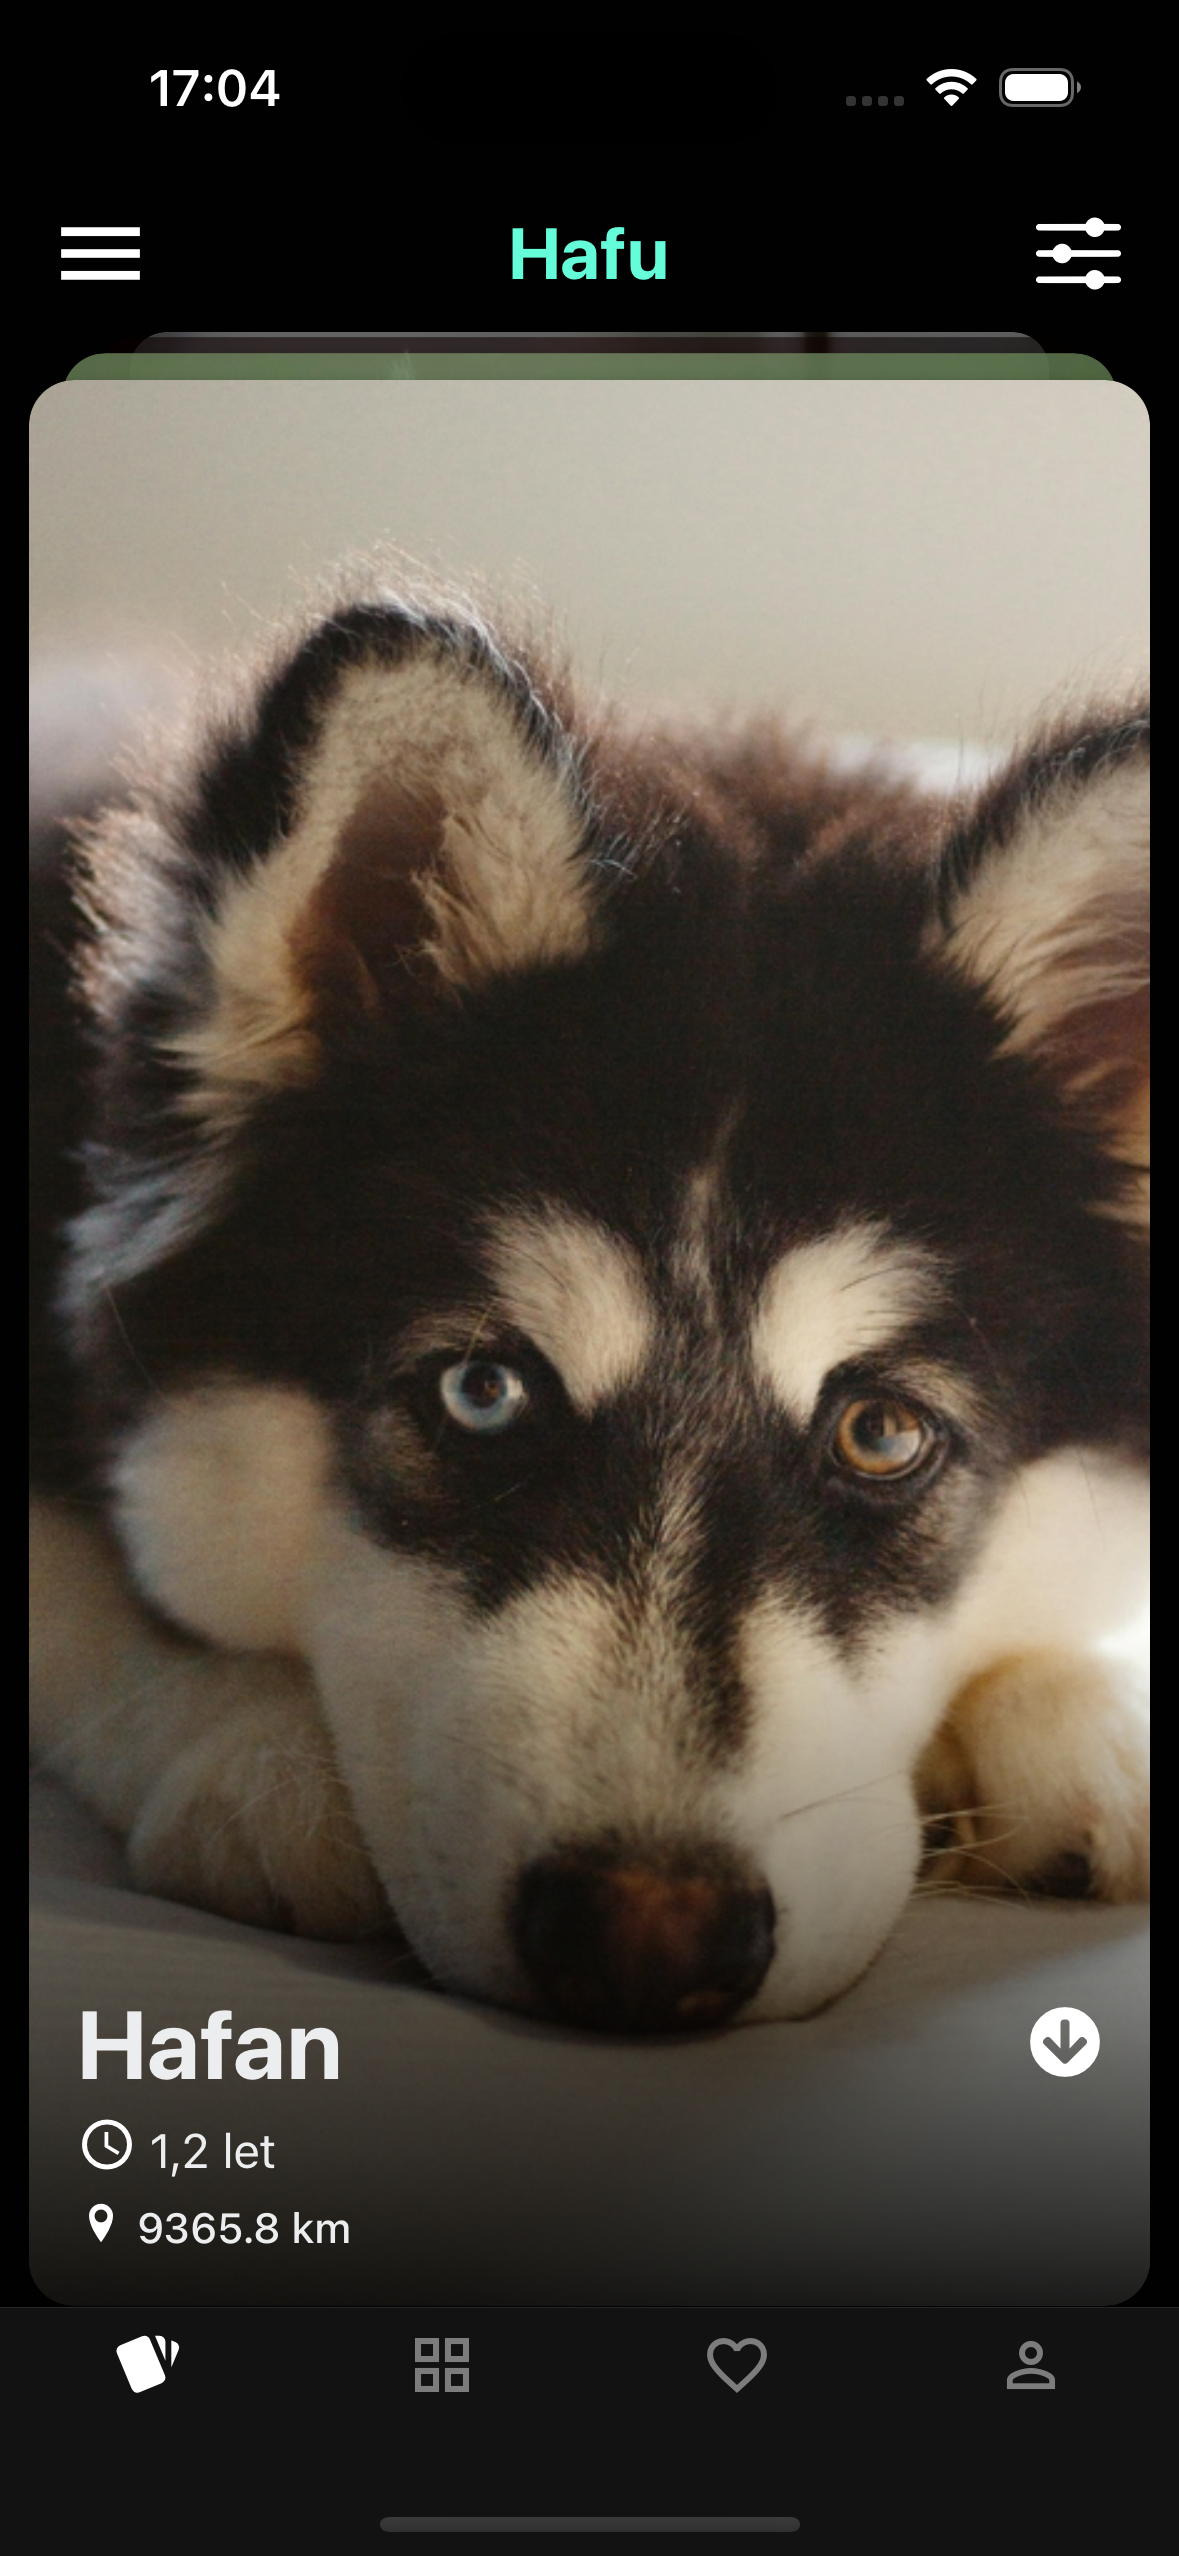
\includegraphics[width=\textwidth]{img-bp/home.png} 
        \caption{Hlavní obrazovka}
        \label{fig:home-page}
    \end{subfigure}
    \hspace{0.05\textwidth}
    \begin{subfigure}{0.3\textwidth}
        \centering
        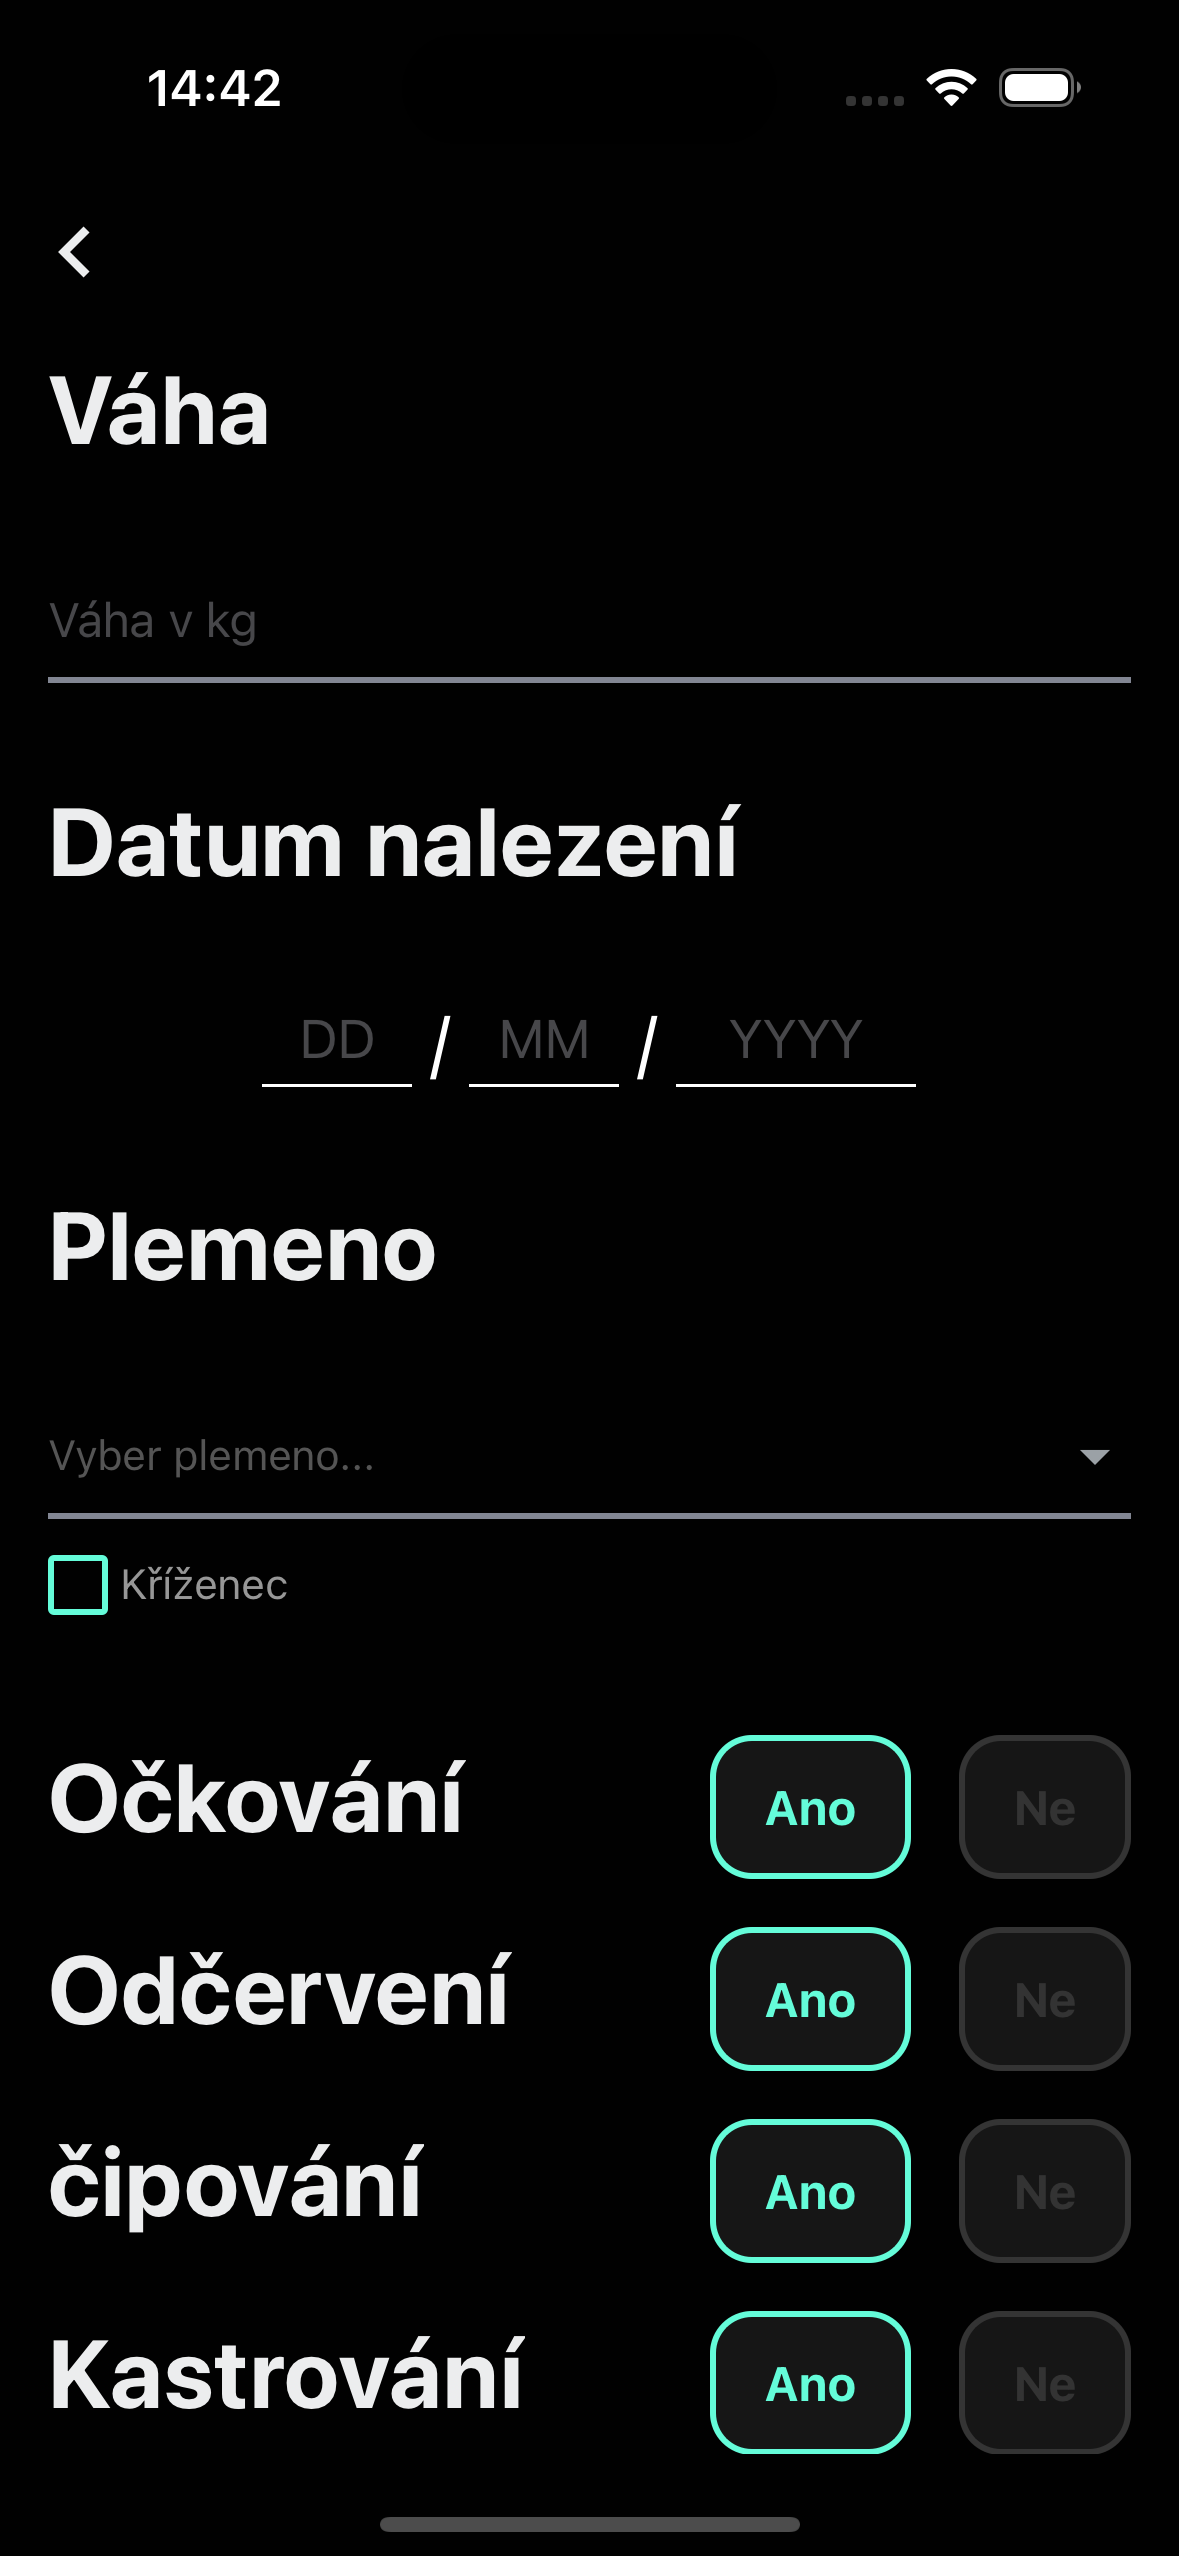
\includegraphics[width=\textwidth]{img-bp/petAdd.png} 
        \caption{Formulář přidání}
        \label{fig:add-pet}
    \end{subfigure}
    \caption{Ukázky obrazovek z hotové mobilní aplikace}
    \label{fig:componets-show}
\end{figure}

\section{Implementace vybraných funkcionalit}

V této sekci jsou detailněji rozebrány některé důležité funkcionality z pohledu implementace a vysvětlení použitých postupů.

\subsection{Autentizace uživatelů}

Registrace a přihlašování byly realizovány pomocí \product{Appwrite SDK}, jak již bylo naznačeno. Implementovali jsme funkci pro přihlášení, která vytváří emailovou relaci, následně získává data o uživateli a ukládá je do kontextu aplikace. V případě chyby je zachycena výjimka a zobrazeno chybové hlášení.

Podobně funkce pro registraci běžného uživatele využívá metodu pro vytvoření uživatelského účtu a poté se může automaticky přihlásit nebo vyzvat uživatele k přihlášení zvlášť. U registrace útulku je postup odlišný v tom, že nejprve vytvoříme uživatele (administrátora) a poté ihned vytváříme záznam v kolekci \textit{shelters}.

Propojení se zajistí tak, že v záznamu útulku v kolekci \textit{shelters} je uložen odkaz na uživatele pomocí pole \textit{owner}, které obsahuje ID uživatelského účtu. Tímto způsobem je vytvořena relace mezi kolekcemi, což je standardní přístup v \product{Appwrite}, kde ID dokumentů jsou generována automaticky. \product{Appwrite} umožňuje definovat tyto relační vazby mezi kolekcemi, což usnadňuje následné dotazování a propojování dat.

Přihlášení kontroluje roli uživatele: po získání informací o uživateli můžeme zjišťovat, zda daný uživatel má odpovídající záznam v \textit{shelters} (například dotazem na kolekci shelters s filtrem pro hledání podle ID uživatele v poli \textit{owner}). Na základě toho aplikace nastaví stav uživatelské role na ``shelter'' nebo ``user'' a podle toho přizpůsobí dostupné obrazovky (útulku například zobrazí navíc boční menu). Toto rozlišení se promítlo i v \product{Expo Router} navigaci – v globálním poskytovateli kontextu je uložena informace o roli a komponenty pro rozložení mohou podmíněně renderovat určité části UI.

\subsection{Načítání a zobrazování dat z Appwrite}

Pro načítání dat, jako je seznam zvířat v sekci Procházet, byl využit hook \textit{useEffect} v kombinaci s \textit{useState}. Ve zjednodušeném postupu vytvoříme stavovou proměnnou pro uložení zvířat, následně pomocí efektu zavoláme funkci pro načtení dat a aktualizujeme stav. 

Funkce pro načtení seznamu zvířat volá příslušnou metodu \product{Appwrite SDK} na kolekci \textit{pets} a vrací pole objektů. Po nastavení stavu se komponenta automaticky překreslí a v renderovací funkci komponenty se vygeneruje uživatelské rozhraní se seznamem karet zvířat. Kliknutí na kartu zajistí přechod na stránku detailu zvířete. 

Podobně ostatní obrazovky načítají data podle potřeby. Důležité bylo ošetřit stav načítání a případné chyby – k tomu slouží komponenta pro zobrazení načítání (například točící se kolečko) a základní zpracování chyb (chyby \product{Appwrite SDK} se například mohou týkat nedostupnosti internetu nebo chybějících oprávnění).

Zobrazování obrázků: komponenta pro zobrazení obrázků z \product{React Native} byla použita pro zobrazování fotografií zvířat. \product{Appwrite Storage} nabízí URL přístup k souborům; pokud byl bucket nastaven jako veřejný pro čtení, stačí znát URL ve standardním formátu obsahujícím koncový bod, ID bucketu, ID souboru a ID projektu. Tyto URL byly generovány na straně klienta pomocí dostupných parametrů. Pokud by byly soukromé, museli bychom buď použít metodu pro náhled souboru s JSON Web Tokenem, nebo vytvořit Cloud Function, která by obrázek zprostředkovala po ověření. V prototypu jsme zvolili veřejné čtení pro zjednodušení.

Obrázky se načítají podle potřeby (lazy loading), přičemž \product{React Native} řeší zobrazení automaticky - pokud není zdroj obrázku okamžitě dostupný, zobrazí zástupný obrázek nebo prázdné místo. \product{Expo} také umožňuje využít techniku \textit{Blurhash} pro zástupné obrázky. V naší implementaci jsme přidali jednoduchý zástupný obrázek (silueta zvířete) pro případ, že konkrétní zvíře ještě nemá fotografii.

\subsection{Filtrace}

Implementace filtrace v aplikaci využívá lokální zpracování dat pro zobrazení relevantních zvířat podle zadaných kritérií. Na rozdíl od filtrování na úrovni databáze, aplikace nejprve načte kompletní seznam zvířat a následně aplikuje uživatelem definované filtry na frontendové části. Tento přístup umožňuje dynamickou a okamžitou filtraci bez nutnosti opakovaných dotazů na server.

Systém filtrace funguje následovně: po načtení kompletního seznamu zvířat z \product{Appwrite} databáze jsou data uložena v lokálním stavu aplikace. Když uživatel nastaví filtrační kritéria, aplikace projde lokální datovou sadu a zobrazí pouze ta zvířata, která odpovídají všem zvoleným parametrům. Tím je zajištěna rychlá odezva a plynulá uživatelská zkušenost při procházení katalogu zvířat.

Uživatelské rozhraní filtrace (viz obrázek \ref{fig:filter}) je navrženo s důrazem na přehlednost a jednoduchost použití. Filtrační kritéria jsou přístupná prostřednictvím tlačítka s ikonou filtru, které po kliknutí otevře modální okno s možnostmi filtrace. Uživatelé mohou specifikovat následující parametry:

\begin{itemize}
\item \textbf{Typ zvířete} - výběr mezi kategoriemi \uv{Vše}, \uv{Psi} a \uv{Kočky}
\item \textbf{Pohlaví} - filtrace podle pohlaví zvířete (Vše, Samec, Samice)
\item \textbf{Věk} - nastavení maximálního věku zvířete s možností volby jednotky (měsíce nebo roky)
\item \textbf{Zdravotní stav} - série přepínačů pro parametry jako očkování, odčervení, čipování, kastrace a přítomnost handicapu
\end{itemize}

Po nastavení požadovaných parametrů a kliknutí na tlačítko \button{POTVRDIT} se okamžitě aplikují filtry na zobrazený seznam zvířat. Tato implementace umožňuje uživatelům rychle přizpůsobit zobrazení podle jejich preferencí bez nutnosti čekat na odpověď ze serveru.

\begin{figure}[h!]
    \centering
    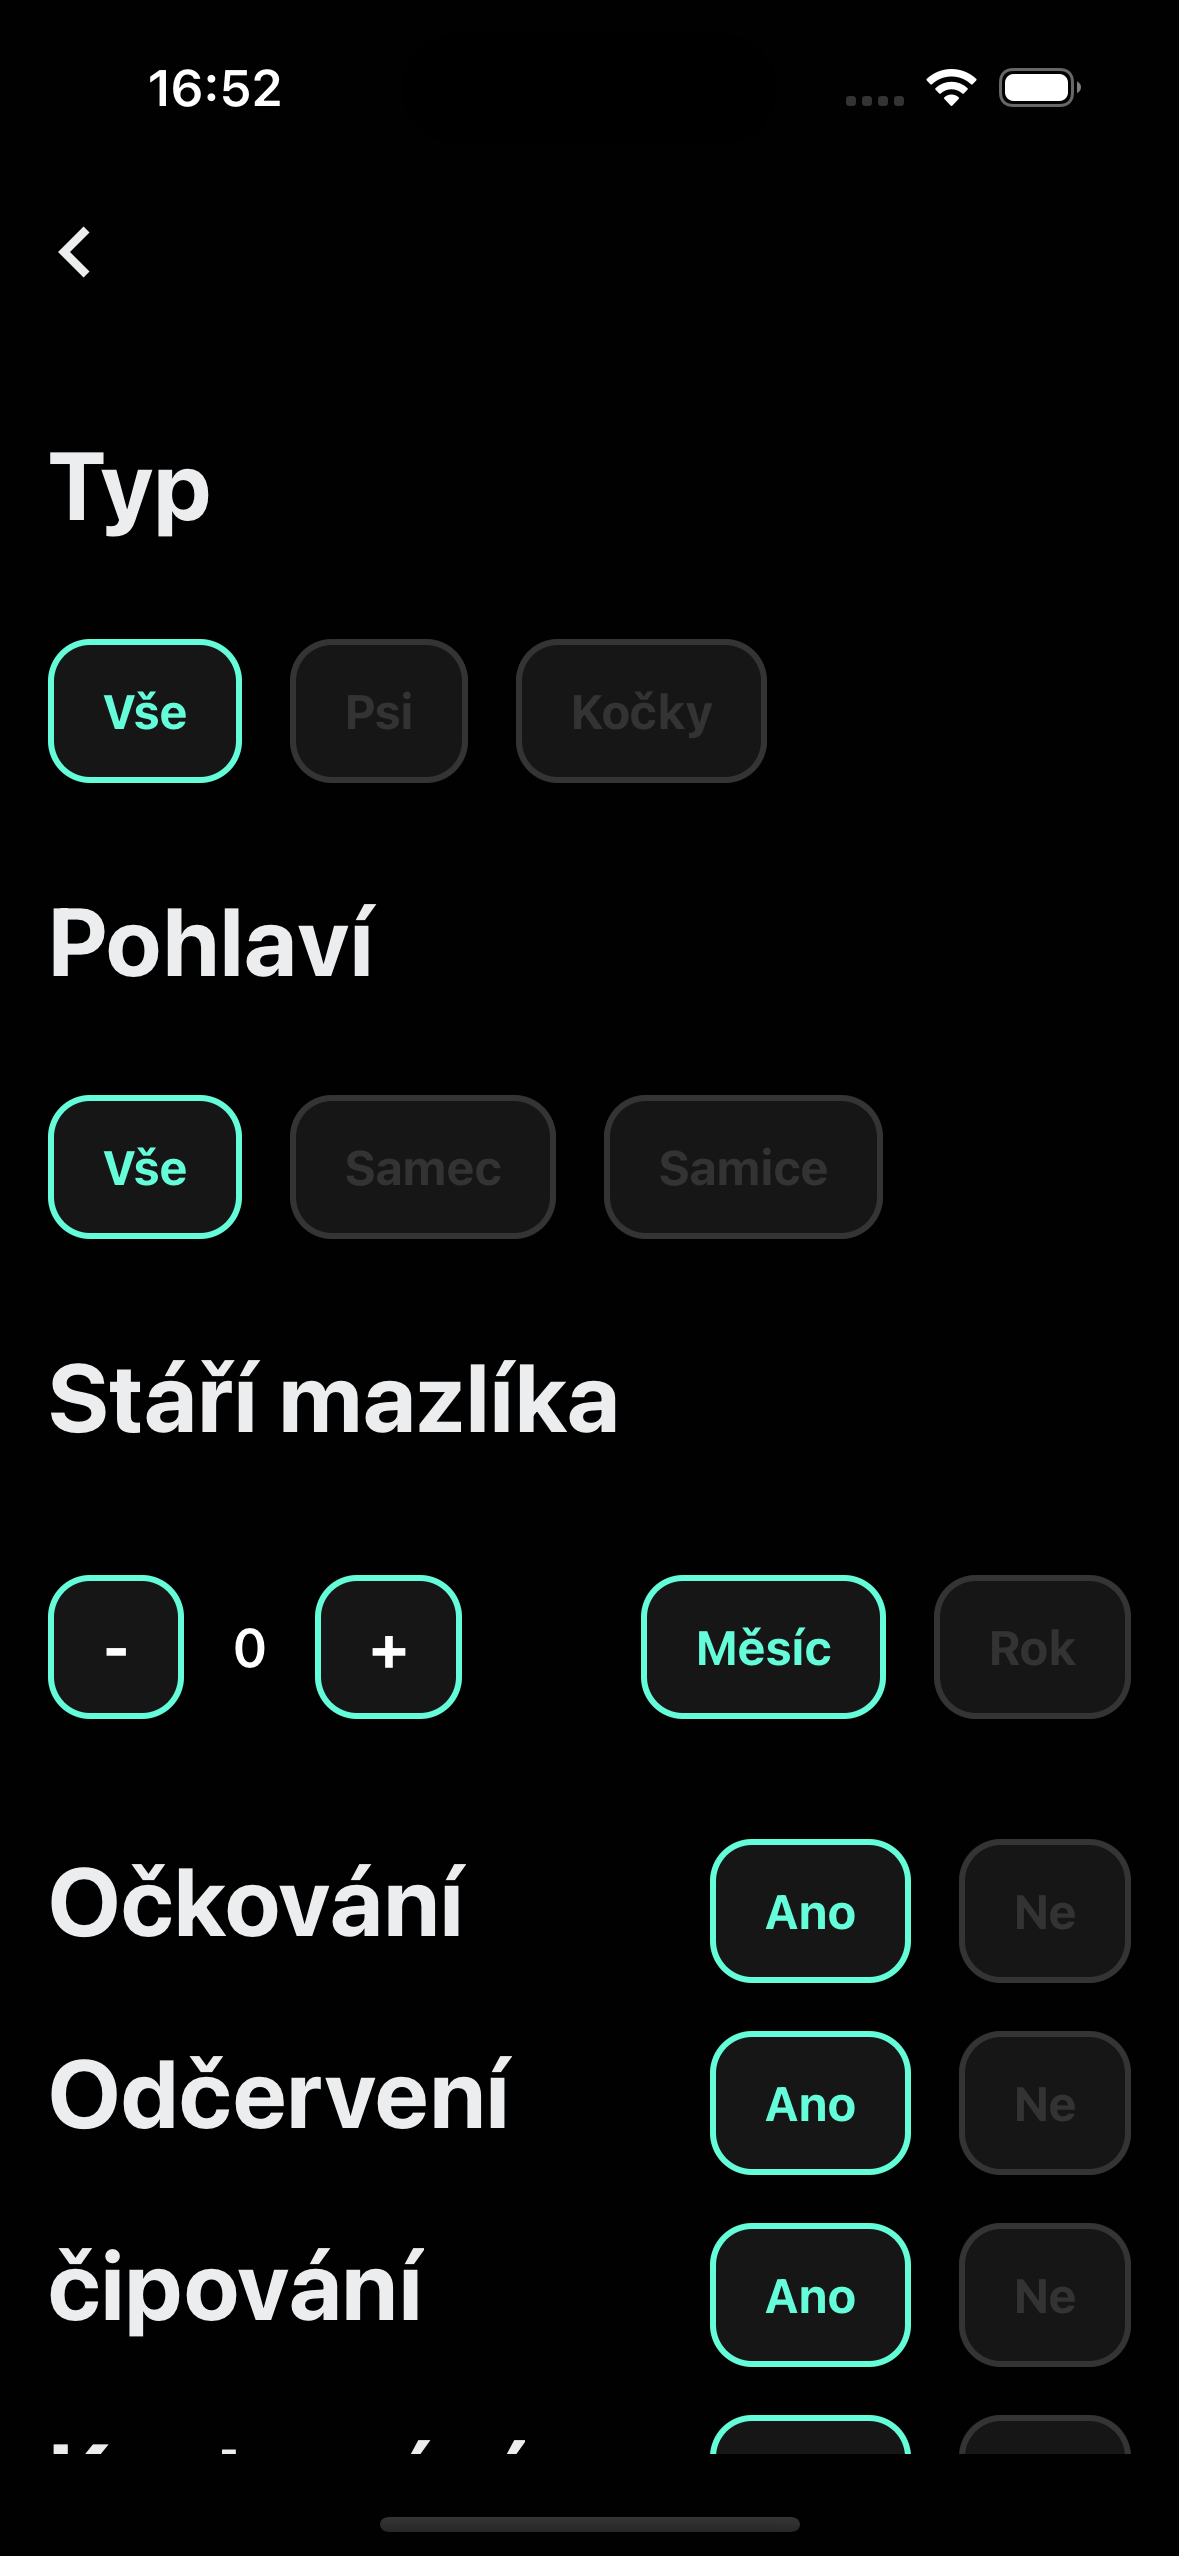
\includegraphics[width=0.3\textwidth]{img-bp/filter.png} 
    \caption{Obrazovka filtru}
    \label{fig:filter}
\end{figure}



\section{Výzvy a zkušenosti z vývoje}

Během vývoje aplikace se objevilo několik zajímavých problémů a výzev, které bylo nutné překonat. Tato sekce popisuje klíčové výzvy a způsoby jejich řešení.


\subsection*{Správa stavu aplikace}

Zpočátku se zdálo výhodné předávat data přes \product{React Context} (například seznam plemen načtený jednou při startu aplikace). Nicméně nadměrné používání kontextu může vést k obtížnějšímu ladění a testování. Vytvořili jsme proto pečlivou strategii vyvažující, co uložit globálně (přihlášený uživatel, základní číselníky) a co vždy dotahovat z API.

Osvědčilo se ukládat v globálním stavu pouze nezbytné minimum a raději optimalizovat dotazy na straně serveru, jelikož \product{Appwrite} nabízí efektivní dotazování a kešování. Pro koordinaci mezi komponentami jsme využili navigační události -- například po úspěšné editaci zvířete a návratu na seznam se spouští \texttt{useEffect} s patřičnou závislostí, který znovu načte aktuální data:

\subsection*{Odladění UI pro různé displeje}

Protože jde o mobilní aplikaci, bylo nutné zajistit správné zobrazení na různých velikostech obrazovek (od menších starších telefonů po moderní zařízení s většími displeji). Implementovali jsme flexibilní styly využívající:

\begin{itemize}
\item Flexbox pro responsivní rozložení prvků
\item Relativní jednotky velikosti (procenta, rem) místo pevných pixelů
\item Komponentu \texttt{ScrollView} pro zajištění přístupu k obsahu i na menších displejích
\item Komponentu \texttt{KeyboardAvoidingView} pro správné chování UI při zobrazení klávesnice
\end{itemize}


\subsection*{Bezpečnost a validace vstupů}

Ačkoliv \product{Appwrite} poskytuje zabezpečení na úrovni backendu (uživatelé nemohou manipulovat s cizími daty díky nastaveným oprávněním), bylo nutné implementovat i kontroly na straně klienta pro lepší uživatelskou zkušenost. Konkrétně jsme zavedli:

\begin{itemize}
\item Validaci formátu emailu při registraci
\item Kontrolu délky a složitosti hesla
\item Ověření vyplnění všech povinných údajů při registraci útulku
\item Validaci hodnot při přidávání a editaci zvířat (datum narození v minulosti, atd.)
\end{itemize}

Validace probíhají před odesláním formuláře a uživatel je upozorněn zvýrazněním chybně vyplněných polí. Z hlediska bezpečnosti je důležité, že heslo uživatele se nikdy neukládá přímo v aplikaci, ale posílá se výhradně přes šifrované spojení (HTTPS) do \product{Appwrite}, kde je bezpečně uloženo v podobě hashe.

Autentizační token je v aktuální verzi aplikace uložen pouze v paměti (v rámci \product{Appwrite SDK}). 

\subsection*{Model propojení uživatelů a útulků}

Složitější architektonickou otázkou bylo, jak efektivně reprezentovat vztah mezi útulkem a jeho správci. \product{Appwrite} má oddělenou správu uživatelů (Accounts) od vlastních databází, což přináší určité výzvy při modelování tohoto vztahu.

Zvažovali jsme využití funkcionality \product{Appwrite Teams}, kde by tým reprezentoval útulek a členové týmu by byli jeho správci. Toto řešení by elegantně propojilo účty s útulky. Vzhledem k časovým možnostem a vyšší implementační náročnosti jsme nakonec zvolili jednodušší přístup: útulek má záznam v kolekci \texttt{shelters} a je propojen s administrátorským účtem pomocí pole \texttt{owner}, které obsahuje ID uživatele.

Současné řešení funguje spolehlivě, ale do budoucna by přechod na model s týmy mohl přinést větší flexibilitu především pro útulky s více správci.

\subsection*{Lokalizace aplikace}

Aplikace je primárně určena pro české prostředí, a proto veškeré texty v uživatelském rozhraní jsou v češtině. Řešení vícejazyčné podpory nebylo v rámci této práce implementováno.

V současné verzi jsou textové řetězce vloženy přímo v kódu komponent. Pro profesionálnější přístup by bylo vhodné použít knihovnu jako \product{i18next} a všechny řetězce extrahovat do samostatných souborů s překlady pro jednotlivé jazyky. Toto bylo identifikováno jako jeden z možných úkolů pro budoucí rozšíření \cite{reacti18next2025}.

\subsection*{Shrnutí zkušeností}

Po překonání výše uvedených výzev se podařilo vytvořit funkční prototyp aplikace splňující stanovené požadavky. Zvolená kombinace technologií se ukázala jako vhodná -- \product{React Native} s \product{Expo} výrazně urychlily vývoj multiplatformního klienta a \product{Appwrite} se osvědčil jako výkonné backendové řešení, které eliminuje potřebu psaní vlastní serverové aplikace.

Implementační zkušenost také identifikovala oblasti, kde by případné pokračování vývoje mohlo aplikaci dále vylepšit, zejména v oblasti perzistence uživatelského stavu, správy útulků s více administrátory a internacionalizace. Tyto možnosti budou detailněji diskutovány v následující kapitole práce.






\chapter{Testování a ověření}

Tato kapitola popisuje způsob testování vyvinuté aplikace a ověření, že splňuje všechny požadavky. Nejprve je představena metodika testování včetně použitých typů testů. Následně jsou uvedeny konkrétní testovací scénáře, které pokrývají hlavní funkčnosti systému, a je shrnuto, s jakými výsledky testy proběhly. Na závěr je zhodnocena spolehlivost a kvalita aplikace na základě testování a navržena případná doporučení pro další zlepšení.

\section{Testovací metodologie}

Pro otestování aplikace byla zvolena kombinace automatizovaných testů a ručního (manuálního) testování podle předem připravených scénářů. Automatizované testy se zaměřily zejména na dílčí jednotky kódu (unit testy) a jednoduché integrační testy komponent, zatímco manuální testování bylo využito pro komplexní scénáře provázející celou aplikaci, uživatelské rozhraní a ověření funkčnosti komunikace s backendem.

\subsection*{Jednotkové testy}

Pro zabezpečení kvality aplikace byly implementovány jednotkové testy, které ověřují správnou funkčnost izolovaných komponent a funkcí. Testování bylo realizováno pomocí frameworku \product{Jest}, který představuje standard pro testování aplikací v~prostředí \product{React Native} \cite{jest2025}.

Testovací soubory byly strukturovány dle konvence do adresáře \texttt{\_\_tests\_\_} v~příslušných složkách projektu. Struktura testů sleduje vzor AAA (Arrange-Act-Assert):

\begin{enumerate}
    \item \textbf{Arrange} - příprava vstupních dat a~testovacího prostředí
    \item \textbf{Act} - volání testované funkce nebo komponenty
    \item \textbf{Assert} - kontrola, zda výsledek odpovídá očekávání
\end{enumerate}

V~rámci testování byly pokryty klíčové utility:
\begin{itemize}
    \item \texttt{dateUtils.ts} - ověření výpočtu věku a~formátování data
    \item \texttt{distanceUtils.ts} - kontrola výpočtu geografické vzdálenosti
    \item \texttt{validation.ts} - testování validačních funkcí pro formuláře
\end{itemize}

Pro komponenty uživatelského rozhraní byly použity techniky mělkého vykreslování (shallow rendering) a~snímkové testy (snapshot tests), které ověřují konzistenci vizuální reprezentace komponent během vývoje aplikace. Simulované události (mock events) umožnily testovat interaktivní chování prvků bez nutnosti reálného uživatelského vstupu.

Testy byly spouštěny automaticky během vývojového procesu pomocí skriptu \texttt{npm test}, což zajistilo včasnou detekci případných regresí. Implementace testů přispěla ke stabilitě aplikace a~umožnila rychlejší a~bezpečnější iterativní vývoj.


\subsection*{Testování podle scénářů}

Hlavním pilířem ověřování funkčnosti bylo manuální testování z pohledu uživatele. Bylo definováno několik testovacích scénářů pokrývajících klíčové use-cases. Každý scénář obsahoval sekvenci kroků, očekávané výsledky a poznámky pro zaznamenání případných odchylek. Scénáře vycházely z požadavků specifikovaných v analytické části a jejich cílem bylo potvrdit, že aplikace splňuje tyto požadavky v praxi.

Pro systematický postup byla využita metoda testování podle uživatelských případů (use case based testing) a rovněž tzv. explorativní testování pro odhalení méně zřejmých chyb. Testovány byly mimo jiné i funkce filtrace zvířat, které umožňují uživatelům zobrazit pouze zvířata odpovídající jejich požadavkům. Testy zahrnovaly jak jednoduché filtrování podle typu zvířete (pes, kočka), tak kombinované filtry podle více kritérií (pohlaví, věk, zdravotní stav).

Testování probíhalo na reálném zařízení (Android smartphone) i v emulátoru, aby se pokryly různé podmínky:
\begin{itemize}
    \item Různá rozlišení obrazovky
    \item Přerušení aplikace při telefonátu
    \item Vypnutí a zapnutí datového připojení
    \item Různé verze operačního systému
    \item Rozdílné rychlosti připojení
\end{itemize}

Po vyplnění filtračních parametrů a stisknutí tlačítka \button{POTVRDIT} byl vždy ověřen výsledný seznam zvířat. Důraz byl kladen nejen na správnost filtrované množiny, ale i na rychlost aplikace filtrů a zachování stavu aplikace při návratu na obrazovku s filtry.

Testováním se ověřuje, že aplikace funguje dle očekávání a že případné chyby jsou odhaleny před nasazením k uživatelům. Důraz byl kladen nejen na správnost funkce, ale i na použitelnost a odolnost vůči nekorektním vstupům.

\section{Testovací scénáře a výsledky}

Níže jsou uvedeny hlavní testovací scénáře společně s výsledky:

\subsection*{Scénář 1: Registrace nového běžného uživatele}

\textbf{Cíl:} Ověřit, že nový zájemce o adopci se může zaregistrovat.\\

\noindent \textbf{Postup:} 
\begin{enumerate}
    \item Otevřít aplikaci, zvolit \button{Přihlásit se jako uživatel} na úvodní obrazovce
    \item Zadat email na první obrazovce a potvrdit tlačítkem \button{POTVRDIT}
    \item Vyplnit jméno a příjmení na druhé obrazovce a potvrdit
    \item Zadat datum narození pomocí výběru (iOS) nebo textových polí (Android)
    \item Vytvořit heslo, zkontrolovat indikátor jeho síly, zadat potvrzení hesla
    \item Potvrdit registraci tlačítkem \button{POTVRDIT}
\end{enumerate}

\noindent \textbf{Očekávání:} Aplikace bude validovat každý krok registračního procesu:
\begin{itemize}
    \item Validace emailu: formát musí obsahovat znak @ a doménu
    \item Validace jména a příjmení: musí obsahovat minimálně 2 znaky, pouze písmena, mezery a pomlčky
    \item Validace data narození: uživatel musí být starší 8 let, datum nesmí být v budoucnosti a nesmí být starší než 120 let
    \item Validace hesla: minimálně 8 znaků, alespoň jedno velké písmeno, jedno malé písmeno, jedna číslice a jeden speciální znak bez mezer
    \item Potvrzení hesla: musí se shodovat s původně zadaným heslem
\end{itemize}

Po úspěšném odeslání všech údajů aplikace vytvoří nový účet a přihlásí uživatele. Na každém kroku očekáváme vhodnou zpětnou vazbu při nesprávných vstupech.\\

\noindent \textbf{Výsledek:} 
Registrace byla otestována s následujícími případy:

\begin{enumerate}
    \item \textbf{Email:} 
    \begin{itemize}
        \item Při zadání neplatného emailu \uv{userexample.com} bez znaku @ systém zobrazil chybovou hlášku \uv{Zadejte platnou emailovou adresu}
        \item Při zadání prázdného pole bylo zobrazeno upozornění \uv{Email je povinný}
        \item Při zadání již existujícího emailu byl uživatel přesměrován na přihlašovací obrazovku
        \item Validní email umožnil přejít na další krok
    \end{itemize}
    
    \item \textbf{Jméno a příjmení:}
    \begin{itemize}
        \item Při pokusu zadat pouze jednopísmenné jméno byla zobrazena chyba \uv{Jméno musí obsahovat alespoň 2 znaky}
        \item Zadání číslic nebo speciálních znaků vyvolalo upozornění \uv{Jméno může obsahovat pouze písmena, mezery a pomlčky}
        \item Při pokusu potvrdit prázdná pole byla zobrazena chyba \uv{Jméno je povinné} a \uv{Příjmení je povinné}
        \item Validní jméno a příjmení umožnilo přejít na další krok
    \end{itemize}
    
    \item \textbf{Datum narození:}
    \begin{itemize}
        \item Na iOS bylo testováno zadání budoucího data, které vyvolalo chybu \uv{Datum narození nemůže být v budoucnosti}
        \item Na Androidu byla testována neplatná kombinace měsíce a roku, což vyvolalo upozornění \uv{Datum narození není platné}
        \item Zadání věku mladšího 8 let vyvolalo upozornění \uv{Musíte být starší 8 let pro registraci}
        \item Validní datum narození umožnilo přejít na další krok
    \end{itemize}
    
    \item \textbf{Heslo:}
    \begin{itemize}
        \item Testováno krátké heslo \uv{abc123}, které vyvolalo chybu \uv{Heslo musí mít alespoň 8 znaků}
        \item Testováno heslo bez velkého písmena, což vyvolalo upozornění \uv{Heslo musí obsahovat alespoň jedno velké písmeno}
        \item Testováno heslo bez speciálního znaku, což vyvolalo upozornění \uv{Heslo musí obsahovat alespoň jeden speciální znak}
        \item Zadání neshodujících se hesel v polích pro heslo a potvrzení hesla vyvolalo chybu \uv{Hesla se neshodují}
        \item Vizuální indikátor síly hesla se měnil z červené (slabé) přes žlutou (střední) na zelenou (silné) podle složitosti zadaného hesla
        \item Validní a silné heslo umožnilo dokončit registraci
    \end{itemize}
\end{enumerate}

Po úspěšném průchodu celým registračním procesem byl vytvořen nový uživatelský účet, jak bylo potvrzeno v \product{Appwrite} konzoli. Uživatel byl automaticky přihlášen a přesměrován na domovskou obrazovku, kde se v profilu zobrazilo jeho jméno. Kompletní registrační proces fungoval dle očekávání a všechny validační kontroly fungovaly správně, zajišťujíce, že pouze validní data jsou přijata. Scénář byl úspěšně splněn bez výskytu jakýchkoli chyb.


\subsection*{Scénář 2: Registrace nového útulku}

\textbf{Cíl:} Ověřit, že nový útulek se může zaregistrovat a vytvořit svůj profil v systému.\\

\noindent \textbf{Postup:} 
\begin{enumerate}
    \item Otevřít aplikaci a kliknout na tlačítko \button{Přihlásit se jako útulek}
    \item V prvním kroku vyplnit základní údaje jako běžný uživatel (jméno, příjmení, e-mail, heslo a datum narození)
    \item Po potvrzení prvního kroku přejít na rozšířený formulář pro útulky a vyplnit:
    \begin{itemize}
        \item Název útulku/organizace
        \item Adresní údaje (ulice, město, PSČ, region)
        \item Kontaktní telefon
        \item Rok založení organizace
        \item Počet zvířat aktuálně v útulku
        \item Počet uskutečněných adopcí za poslední rok
        \item Popis útulku a jeho činnosti
        \item Nahrát alespoň jednu fotografii zařízení
        \item Registrační číslo Státní veterinární správy (volitelné pole)
    \end{itemize}
    \item Potvrdit registraci tlačítkem \button{POTVRDIT}
\end{enumerate}

\noindent \textbf{Očekávání:} Aplikace umožní vyplnit všechny požadované údaje ve dvou navazujících formulářích, provede validaci vstupů (zejména ověření e-mailu a povinných polí), a po odeslání formuláře vytvoří nový profil útulku. Po úspěšné registraci bude útulek přihlášen a přesměrován na svou domovskou stránku s rozšířenými funkcemi pro správu zvířat.\\

\noindent \textbf{Výsledek:} 
Registrace proběhla úspěšně. Testována byla následující validační kritéria:
\begin{itemize}
    \item Při nevyplnění povinných polí (název útulku, adresa, telefon) systém zobrazil upozornění \uv{Vyplňte prosím všechny povinné údaje} a zvýraznil chybějící položky červeným orámováním
    \item Při zadání neplatného telefonního čísla systém zobrazil upozornění \uv{Zadejte platné telefonní číslo}
    \item Při zadání roku založení mimo platný časový rozsah (1800 až současný rok) systém správně zobrazil validační upozornění s textem \uv{Rok vzniku není platný}.
    \item Při pokusu o nahrání fotografie ve formátu, který není podporován, systém zobrazil upozornění \uv{Nepodporovaný formát souboru, použijte JPG nebo PNG}
\end{itemize}

Po úspěšném vyplnění všech údajů a odeslání formuláře byl vytvořen nový účet útulku, což bylo ověřeno i v \product{Appwrite} konzoli. Uživatel byl automaticky přihlášen do aplikace a přesměrován na domovskou obrazovku s rozšířeným bočním menu pro správu zvířat a profilu útulku. V profilu byly správně zobrazeny všechny zadané údaje včetně nahrané fotografie. Scénář splněn, žádná chyba se nevyskytla.



\subsection*{Scénář 3: Přihlášení a odhlášení}

\textbf{Cíl:} Test správnosti přihlášení existujícího uživatele a možnosti se odhlásit.\\

\noindent \textbf{Postup:} 
\begin{enumerate}
    \item Spustit aplikaci a na úvodní obrazovce zvolit přihlášení
    \item Zadat registrovaný email a heslo do příslušných polí
    \item Stisknout tlačítko \button{Přihlásit se jako uživatel}
    \item Po úspěšném přihlášení otestovat dostupnost sekcí aplikace podle role uživatele
    \item Přejít do sekce profilu a stisknout tlačítko \button{ODHLÁSIT}
    \item Ověřit, že uživatel byl skutečně odhlášen a nemá přístup k chráněným částem aplikace
\end{enumerate}

\noindent \textbf{Očekávání:} Aplikace provede validaci přihlašovacích údajů. Email musí být ve správném formátu (obsahovat znak @ a doménu), heslo musí odpovídat uloženému heslu uživatele. Po úspěšném přihlášení se zobrazí obsah aplikace odpovídající roli uživatele. U běžného uživatele bude dostupná navigace se sekcemi Domů, Procházet, Oblíbené a Profil. U útulku bude navíc přístupné boční menu se správou zvířat a profilem útulku. Po odhlášení bude uživatel přesměrován na přihlašovací obrazovku, autentizační token bude zneplatněn a přístup k chráněným částem aplikace bude odepřen.\\

\noindent \textbf{Výsledek:} 
Přihlašování bylo testováno s následujícími případy:
\begin{itemize}
    \item Při zadání neregistrovaného emailu nebo špatného hesla byla zobrazena chybová hláška \uv{Nesprávné přihlašovací údaje}.
    \item Při pokusu o přihlášení s prázdným emailem systém zobrazil chybu \uv{Email je povinný}, při prázdném heslu pak \uv{Heslo je povinné}.
    \item Při zadání emailu v nesprávném formátu (bez znaku @) systém zobrazil chybu \uv{Zadejte platnou emailovou adresu}.
\end{itemize}



\subsection*{Scénář 4: Označení oblíbeného a zobrazení v seznamu Oblíbené}

\textbf{Cíl:} Ověření funkce označení zvířete jako oblíbeného a jeho následného zobrazení v sekci oblíbených.\\

\noindent \textbf{Postup:} 
\begin{enumerate}
    \item Přihlásit se jako běžný uživatel
    \item Na domovské obrazovce procházet karty zvířat a označit několik z nich jako oblíbené (swipe doprava nebo stisknutí ikony srdce v detailu zvířete)
    \item Přejít do sekce \button{Oblíbené} pomocí spodní navigace
    \item Ověřit, že označená zvířata se zobrazují v seznamu
    \item Otevřít detail jednoho z oblíbených zvířat
    \item Zkusit odebrat zvíře z oblíbených stisknutím ikony srdce v detailu
    \item Vrátit se zpět na seznam oblíbených a ověřit, že zvíře bylo odebráno
    \item Odhlásit se, znovu se přihlásit a ověřit, že oblíbená zvířata zůstala zachována
\end{enumerate}

\noindent \textbf{Očekávání:} Systém spolehlivě ukládá informace o oblíbených zvířatech. Označená zvířata se ihned zobrazí v sekci \button{Oblíbené}. Tato informace je persistentně uložena v databázi a zůstává zachována i po odhlášení a opětovném přihlášení. Zrušení označení zvířete jako oblíbeného se projeví okamžitým odstraněním ze seznamu oblíbených. Uživatel nemůže opakovaně označit stejné zvíře jako oblíbené.\\

\noindent \textbf{Výsledek:} 
Test prokázal, že funkcionalita oblíbených zvířat funguje spolehlivě. Uživatel úspěšně označil 2 zvířata jako oblíbená pomocí swipe gesta doprava na domovské obrazovce. Tyto záznamy se okamžitě objevily v sekci \button{Oblíbené}, kde byly zobrazeny jako karty s informacemi o zvířeti včetně fotografie, věku a dalších detailů.

Když uživatel kliknul na kartu, otevřel se detail zvířete se všemi informacemi. V detailu bylo možné zvíře odebrat z oblíbených kliknutím na ikonu srdce (která byla vyplněná, což indikovalo aktuální stav). Po kliknutí se ikona změnila na nevyplněnou a po návratu na seznam oblíbených bylo ověřeno, že zvíře již v seznamu není.

Po odhlášení a opětovném přihlášení do aplikace zůstávalo zbývající oblíbené zvíře v seznamu, což potvrdilo správnou persistenci dat v databázi (záznamy byly uloženy v kolekci \textit{user\_pet\_actions}). 

Dále bylo ověřeno, že systém správně zamezuje duplicitním označením - když se uživatel pokusil označit stejné zvíře jako oblíbené podruhé, akce byla ignorována nebo jen přepnula existující stav mezi oblíbené/neoblíbené. 

Test také potvrdil, že filtrace oblíbených zvířat funguje správně, pokud byl nastaven filtr v sekci \button{Oblíbené}, zobrazila se pouze ta zvířata, která vyhovovala kritériím filtru (např. podle typu, věku, zdravotního stavu).


\subsection*{Scénář 5: Přidání nového zvířete útulkem}

\textbf{Cíl:} Test administrátorské funkce přidání nového zvířete do databáze útulkem.\\

\noindent \textbf{Postup:} 
\begin{enumerate}
    \item Přihlásit se do aplikace jako útulek
    \item Přejít do sekce \button{Správa zvířat} pomocí bočního menu
    \item Kliknout na tlačítko \button{Přidat nové}
    \item Vyplnit formulář s údaji o zvířeti:
    \begin{itemize}
        \item Typ zvířete: Pes
        \item Jméno: \uv{Bobík}
        \item Pohlaví: Samec
        \item Měsíc a rok narození: Leden 2023
        \item Velikost: Střední
        \item Váha: 8,5 kg
        \item Plemeno: Jezevčík
        \item Zdravotní stav (přepínače Ano/Ne): 
        \begin{itemize}
            \item Očkování: Ano
            \item Odčervení: Ano
            \item Čipování: Ano
            \item Kastrace: Ne
            \item Handicap: Ne
        \end{itemize}
        \item Popis zvířete: \uv{Bobík je přátelský a hravý pejsek, který miluje dlouhé procházky a aportování. Je vhodný k~dětem i jiným zvířatům.}
        \item Adopční poplatek: 1500 CZK
    \end{itemize}
    \item Nahrát alespoň jednu fotografii zvířete
    \item Stisknout tlačítko \button{POTVRDIT}
    \item Odhlásit se a přihlásit se jako běžný uživatel
    \item Ověřit, zda je nově přidané zvíře viditelné v~katalogu
\end{enumerate}

\noindent \textbf{Očekávání:} 
Aplikace bude během vyplňování formuláře validovat vstupní údaje. Po úspěšném odeslání formuláře bude zvíře přidáno do databáze a bude viditelné jak v~seznamu zvířat daného útulku, tak v~katalogu pro běžné uživatele. Systém by měl být odolný vůči nestabilnímu internetovému připojení a poskytovat adekvátní zpětnou vazbu při validačních chybách.\\

\noindent \textbf{Výsledek:} 
Test přidání nového zvířete proběhl úspěšně s~několika poznámkami k~uživatelskému rozhraní. Během testování bylo ověřeno následující:

\begin{itemize}
    \item Při pokusu o odeslání formuláře s~nevyplněným jménem zvířete aplikace zabránila uložení a červeně zvýraznila povinné pole. Podobně reagovala na chybějící povinná data jako typ zvířete, velikost (u psů) a chybějící fotografii.
    
    \item Při zadání záporné váhy systém zobrazil chybovou hlášku \uv{Váha musí být alespoň 0}. Při zadání nevalidního data (např. 30. února) byl zobrazen chybový stav.
    
    \item Nahrání fotografie proběhlo standardně, aplikace umožnila vybrat obrázek z~galerie zařízení. Po výběru obrázku byl tento zobrazen v~náhledu.
    
    \item Po korektním vyplnění všech polí a stisku \button{POTVRDIT} trvalo zpracování požadavku přibližně 1-2 sekundy, po nichž byl zobrazen potvrzovací dialog o úspěšném přidání zvířete. 
    
    \item Po přihlášení jako běžný uživatel bylo nově přidané zvíře \uv{Bobík} okamžitě viditelné v~katalogu se všemi zadanými údaji a nahranou fotografií.
\end{itemize}

Formulář a proces přidání nového zvířete fungoval spolehlivě. Všechny validační mechanismy pracovaly správně, čímž zabránily vložení nekorektních dat do systému. Menší nedostatek byl pozorován pouze v~podobě chybějícího indikátoru průběhu při nahrávání větších souborů fotografií. Tento scénář potvrdil plnou funkčnost klíčové administrátorské funkce pro útulky.



\subsection*{Scénář 6: Editace záznamu zvířete}

\textbf{Cíl:} Ověřit možnost aktualizace údajů u existujícího zvířete útulkem.\\

\noindent \textbf{Postup:} 
\begin{enumerate}
    \item Přihlásit se do aplikace jako útulek
    \item Přejít do sekce \button{Správa zvířat} v bočním menu
    \item Ze seznamu vybrat zvíře a otevřít jeho detail
    \item Kliknout na tlačítko \button{Upravit}
    \item Provést několik změn:
    \begin{itemize}
        \item Upravit textový popis zvířete
        \item Změnit váhu zvířete
        \item Aktualizovat stav očkování a odčervení
        \item Nahrát novou fotografii
    \end{itemize}
    \item Uložit změny tlačítkem \button{POTVRDIT}
    \item Ověřit, že změny se zobrazují v detailu zvířete
    \item Odhlásit se a přihlásit jako běžný uživatel
    \item Vyhledat upravené zvíře v katalogu a ověřit, že změny jsou viditelné
\end{enumerate}

\noindent \textbf{Očekávání:} 
Formulář pro editaci bude naplněn existujícími údaji zvířete. Aplikace umožní změnit libovolné údaje a po potvrzení budou změny uloženy do databáze. Validace formuláře zajistí kontrolu dat (např. váha nemůže být záporná, popis nemůže přesáhnout 500 znaků). Po úspěšném uložení by měly být změny okamžitě viditelné v detailu zvířete a po aktualizaci i v katalogu pro běžné uživatele.\\

\noindent \textbf{Výsledek:} 
Editace záznamu zvířete proběhla úspěšně. Po otevření formuláře byly správně předvyplněny všechny údaje včetně:
\begin{itemize}
    \item Jméno a identifikátor zvířete
    \item Data narození (měsíc a rok)
    \item Vybraná velikost (u psů)
    \item Aktuální váha
    \item Zdravotní údaje (očkování, odčervení, čipování, kastrace a případný handicap)
    \item Textový popis zvířete
    \item Adopční poplatek a měna
    \item Již nahrané fotografie
\end{itemize}

Při testování byla provedena změna popisu zvířete, aktualizace jeho váhy z 10 kg na 8,5 kg, změna stavu očkování z \uv{Ne} na \uv{Ano} a nahrání nové fotografie. Všechny úpravy byly validovány – při pokusu zadat zápornou hodnotu váhy systém zobrazil chybovou hlášku \uv{Váha musí být alespoň 0}.

Po stisknutí tlačítka \button{POTVRDIT} aplikace zobrazila potvrzovací dialog o úspěšné aktualizaci a změny byly okamžitě viditelné v detailu zvířete. Při přihlášení jako běžný uživatel a otevření katalogu (po refresh) byly všechny změny správně zobrazeny.



\subsection*{Scénář 7: Aktualizace údajů uživatelského účtu}

\textbf{Cíl:} Ověřit možnost editace osobních údajů, změny emailu a hesla uživatelem.\\

\noindent \textbf{Postup:} 
\begin{enumerate}
    \item Přihlásit se do aplikace jako běžný uživatel
    \item Přejít do sekce uživatelského profilu
    \item Kliknout na tlačítko \button{Upravit účet}
    \item Postupně vyzkoušet jednotlivé sekce úprav:
    \begin{itemize}
        \item Změna jména a příjmení
        \item Změna emailové adresy (vyžaduje zadání současného hesla)
        \item Změna hesla (vyžaduje zadání současného hesla a dvakrát nového hesla)
    \end{itemize}
    \item U každé sekce provést validační testy (neplatné údaje, prázdná pole)
    \item Po úspěšné editaci ověřit, že změny byly uloženy
\end{enumerate}

\noindent \textbf{Očekávání:} 
Aplikace umožní úpravu jednotlivých údajů, přičemž každá sekce bude mít vlastní validační mechanismy. Změna údajů vyžadujících zvýšenou bezpečnost (email, heslo) bude podmíněna zadáním současného hesla pro ověření identity. Uživateli bude poskytována jasná zpětná vazba o výsledku operací. Nové heslo bude kontrolováno na dostatečnou komplexnost a při změně hesla bude vyžadováno jeho potvrzení zadáním ve druhém poli.\\

\noindent \textbf{Výsledek:} 
Test aktualizace údajů proběhl úspěšně s následujícími poznatky:

\begin{itemize}
    \item \textbf{Změna jména a příjmení:}
    \begin{itemize}
        \item Při pokusu zadat jednopísmenné jméno aplikace zobrazila chybu \uv{Jméno musí obsahovat alespoň 2 znaky}
        \item Při zadání číslic nebo speciálních znaků do jména bylo zobrazeno upozornění \uv{Jméno může obsahovat pouze písmena, mezery a pomlčky}
        \item Při validním vstupu a kliknutí na \button{ULOŽIT} byla změna úspěšně provedena a potvrzena vyskakovacím dialogem
        \item Po opětovném načtení profilu bylo ověřeno, že nové jméno a příjmení bylo správně uloženo
    \end{itemize}
    
    \item \textbf{Změna emailové adresy:}
    \begin{itemize}
        \item Při zadání nevalidního formátu emailu aplikace zobrazila chybu \uv{Zadejte platnou emailovou adresu}
        \item Při pokusu o změnu emailu bez zadání současného hesla systém zobrazil upozornění \uv{Pro změnu emailu je potřeba zadat současné heslo}
        \item Při zadání nesprávného hesla byla zobrazena chyba \uv{Zadané heslo není správné}
        \item Při zadání stejného emailu jako současného se zobrazila informace \uv{Email se nezměnil}
        \item Po úspěšné změně (validní email a správné heslo) byl zobrazen potvrzovací dialog a po přihlášení byl viditelný nový email
    \end{itemize}
    
    \item \textbf{Změna hesla:}
    \begin{itemize}
        \item Při nevyplnění současného hesla aplikace zobrazila upozornění \uv{Současné heslo je povinné}
        \item Při zadání krátkého hesla (méně než 8 znaků) byla zobrazena chyba \uv{Heslo musí mít alespoň 8 znaků}
        \item Při zadání hesla bez speciálního znaku, velkého písmene nebo číslice bylo zobrazeno příslušné upozornění
        \item Vizuální indikátor síly hesla měnil barvu podle složitosti (červená pro slabé, žlutá pro střední, zelená pro silné heslo)
        \item Při zadání odlišných hesel do polí pro nové heslo a potvrzení hesla byla zobrazena chyba \uv{Hesla se neshodují}
        \item Po úspěšné změně hesla bylo zobrazeno potvrzení a následné přihlášení s novým heslem fungovalo správně
    \end{itemize}
\end{itemize}

Veškeré validační mechanismy fungovaly správně, uživatelské rozhraní poskytovalo jasnou zpětnou vazbu o průběhu operací. Po provedení změn byly údaje správně aktualizovány v databázi a promítly se do uživatelského profilu. Test potvrdil, že funkcionalita pro aktualizaci údajů účtu je implementována bezpečně a uživatelsky přívětivě.





\subsection*{Scénář 8: Aktualizace údajů profilu útulku}

\textbf{Cíl:} Ověřit možnost úpravy informací o útulku včetně základních údajů, kontaktů a fotografií.\\

\noindent \textbf{Postup:} 
\begin{enumerate}
    \item Přihlásit se do aplikace jako útulek (administrátor útulku)
    \item V hlavní nabídce přejít do sekce profilu útulku
    \item Zvolit možnost \button{Upravit profil}
    \item Provést změny v několika údajích:
    \begin{itemize}
        \item Aktualizovat popis útulku
        \item Změnit kontaktní telefonní číslo
        \item Upravit adresu
        \item Aktualizovat počet zvířat v útulku
        \item Nahrát novou fotografii útulku
    \end{itemize}
    \item Uložit změny stisknutím tlačítka \button{POTVRDIT}
    \item Zkontrolovat, zda se změny projevily v profilu útulku
    \item Odhlásit se a přihlásit jako běžný uživatel
    \item Vyhledat útulek v seznamu a ověřit, že změny jsou viditelné i pro běžné uživatele
\end{enumerate}

\noindent \textbf{Očekávání:} 
Aplikace umožní správci útulku upravit všechny informace o útulku, které byly zadány při registraci. Po uložení změn budou aktualizované údaje okamžitě dostupné v profilu útulku a budou správně zobrazeny i běžným uživatelům při prohlížení detailu útulku nebo při prohlížení zvířat náležících k danému útulku. Systém by měl provést validaci vstupních údajů (např. formát telefonního čísla, délka popisu) a zajistit bezproblémové nahrání a zobrazení nové fotografie útulku.\\

\noindent \textbf{Výsledek:} 
Test aktualizace údajů útulku proběhl úspěšně. Při pokusu aktualizovat profil útulku byly testovány následující případy:
\begin{itemize}
    \item \textbf{Popis útulku:} Úspěšně aktualizován delším a podrobnějším textem, který byl následně správně zobrazen ve formátovaném bloku na profilu útulku.
    
    \item \textbf{Kontaktní údaje:} Při zadání nevalidního telefonního čísla (např. obsahujícího písmena) systém zobrazil upozornění \uv{Zadejte platné telefonní číslo} a zvýraznil pole červeným orámováním. Po zadání správného formátu byla změna úspěšně uložena.
    
    \item \textbf{Adresa:} Aktualizace adresy proběhla bez problémů, změněná adresa se okamžitě projevila na detailu útulku a byla správně použita i při zobrazení na mapě.
    
    \item \textbf{Počet zvířat:} Úprava počtu zvířat byla validována (pouze kladná celá čísla) a po uložení byla změna viditelná v informačním panelu profilu útulku.
    
    \item \textbf{Fotografie útulku:} Při nahrávání nové fotografie systém podporoval běžné formáty (JPG, PNG), nepřijal však příliš velké soubory (>5 MB) a zobrazil příslušné upozornění. Po nahrání vhodné fotografie byla tato okamžitě viditelná v galerii profilu útulku.
\end{itemize}

Po odhlášení a přihlášení jako běžný uživatel bylo ověřeno, že všechny provedené změny jsou viditelné také z pohledu běžného uživatele při prohlížení detailů útulku a zvířat. Aplikace také správně aktualizovala údaje v databázi \product{Appwrite}, což bylo ověřeno v administračním rozhraní. Tento scénář potvrdil, že funkce aktualizace profilu útulku pracuje spolehlivě a umožňuje útulkům udržovat své údaje aktuální.



\subsection*{Scénář 9: Vyhledávání a filtrování}

\textbf{Cíl:} Otestovat komplexní funkčnost filtračního systému pro katalog zvířat.\\

\noindent \textbf{Postup:} 
\begin{enumerate}
    \item Přihlásit se do aplikace jako běžný uživatel
    \item Přejít do sekce \button{Procházet} nebo \button{Domů}
    \item Kliknout na ikonu filtru v pravém horním rohu obrazovky
    \item V dialogu filtru postupně otestovat jednotlivé filtrační kritéria:
    \begin{itemize}
        \item Typ zvířete (Vše, Psi, Kočky)
        \item Pohlaví (Vše, Samec, Samice)
        \item Stáří mazlíka (nastavit hodnotu v měsících nebo letech)
        \item Zdravotní stav (očkování, odčervení, čipování, kastrace, handicap)
    \end{itemize}
    \item Potvrdit nastavení filtru tlačítkem \button{POTVRDIT}
    \item Ověřit, že zobrazená zvířata odpovídají zadaným kritériím
    \item Vyzkoušet kombinaci více filtrů současně
    \item Opakovat proces v různých sekcích aplikace (Domů, Procházet)
\end{enumerate}

\noindent \textbf{Očekávání:} 
Aplikace by měla umožnit nastavení různých filtračních kritérií a po potvrzení filtru zobrazit pouze zvířata, která splňují všechna zadaná kritéria. Filtrování by mělo být konzistentní napříč různými obrazovkami aplikace. Výsledky by se měly zobrazit rychle a měly by přesně odpovídat nastaveným filtrům.\\

\noindent \textbf{Výsledek:} 
Testování filtrační funkcionality odhalilo robustní a efektivní implementaci. Filtrování probíhalo následovně:

\begin{itemize}
    \item \textbf{Filtr typu zvířete:} Při výběru kategorie \uv{Psi} byly zobrazeny pouze záznamy psů, při volbě \uv{Kočky} pouze kočky. Možnost \uv{Vše} zobrazila kompletní seznam bez ohledu na typ.
    
    \item \textbf{Filtr pohlaví:} Výběr \uv{Samec} nebo \uv{Samice} správně filtroval zvířata podle odpovídajícího pohlaví. Fungovala i kombinace s ostatními filtry (např. samice kočky).
    
    \item \textbf{Filtr stáří:} Nastavení maximálního věku 2 roky zobrazilo pouze zvířata mladší než zadaná hodnota. Přepínání mezi měsíci a roky fungovalo korektně a systém správně přepočítával věk z data narození zvířete.
    
    \item \textbf{Filtry zdravotního stavu:} Volba \uv{Ano} u očkování zobrazila pouze očkovaná zvířata, stejný princip fungoval i u ostatních zdravotních parametrů (odčervení, čipování, kastrace, handicap).
\end{itemize}

Kombinace více filtrů současně fungovala správně – aplikace zobrazila pouze zvířata, která splňovala všechna vybraná kritéria. Například filtr \uv{Psi + Samec + Očkování Ano} zobrazil pouze psy, kteří jsou samci a zároveň očkovaní.

Filtrační systém pracoval konzistentně na obrazovkách \texttt{Domů} (swipe karty) i \texttt{Procházet} (mřížka karet). Odezva systému byla rychlá, filtrace probíhala téměř okamžitě po stisknutí tlačítka \button{POTVRDIT}. Dotazy směřované na backend \product{Appwrite} byly zpracovány efektivně.

Jediným námětem na vylepšení je uživatelské rozhraní filtrů – bylo by vhodné doplnit vizuální indikaci aktivního filtru (např. barevný štítek nebo čítač aktivních filtrů v záhlaví), aby uživatel byl informován, že aktuálně nevidí kompletní seznam zvířat, ale pouze filtrovanou podmnožinu.






\section{Zhodnocení a spolehlivost systému}

Na základě testování lze konstatovat, že aplikace je funkční a stabilní. Splňuje účel, pro který byla navržena -- propojuje útulky a zájemce o adopci prostřednictvím přehledné mobilní platformy. Automatizované testy budou nadále užitečné při dalším vývoji, neboť zajistí, že nové úpravy nenaruší stávající funkcionalitu (tzv. regresní testování). Manuální testování samozřejmě bude potřeba opakovat s každou významnější změnou či před nasazením nové verze koncovým uživatelům.

Postupem času by bylo vhodné rozšířit sadu testů, zejména o integrační/E2E testy, aby se ověřila i vizuální a interakční stránka aplikace automatizovaně. Celkově testování potvrdilo, že aplikace reaguje správně i na neočekávané situace (např. výpadek připojení, pokus o akci bez oprávnění).

Podobně systém zamezuje i vzniku nekonzistentních dat díky nastaveným omezením (unikátní klíče, vazby mezi kolekcemi atd.), takže například nelze vložit duplicitní záznam plemene či vytvořit dva identické ``like'' záznamy pro jednoho uživatele a zvíře.

Z pohledu \textit{uživatelské zkušenosti} (UX) byla aplikace hodnocena v neformálních testech několika dobrovolníky jako intuitivní -- ovládání přes taby a karty bylo pochopitelné, design odpovídá běžným zvyklostem. Z technického hlediska se potvrdilo, že zvolená architektura je stabilní a díky využití hotových backendových služeb odpadla řada potenciálních problémů (např. zabezpečení databáze, správa uživatelů) -- to vše řeší \product{Appwrite} automatizovaně.

Samozřejmě je možné systém dále vylepšovat, nicméně již v současné podobě představuje použitelný produkt. Testování přispělo k odhalení chyb a ověření kvality, čímž splnilo svůj účel -- ostatně právě proto je důsledné testování nezbytnou součástí vývoje kvalitních aplikací.




\chapter{Budoucí rozšíření}

Vzhledem k omezenému rozsahu bakalářské práce nebylo možné implementovat všechny zamýšlené funkce a vylepšení. Tato kapitola nastiňuje možné směry budoucího rozvoje aplikace. Nejprve jsou diskutovány potenciální nové funkčnosti, které by zvýšily užitnou hodnotu aplikace pro uživatele i útulky. Poté jsou rozebrány možnosti integrace aplikace s externími systémy a otázky škálování – tedy připravenost systému růst s počtem uživatelů a dat.

\section{Návrhy nových funkcí}

\subsection*{Integrovaná komunikace}

Jedním z nejdůležitějších rozšíření by bylo přidání interního komunikačního modulu (chat) mezi zájemcem a útulkem. V současné verzi aplikace je kontakt realizován mimo systém (telefonicky nebo e-mailem), což je funkční, ale méně pohodlné. Vestavěný \textit{chat} nebo zasílání zpráv by umožnilo uživatelům komunikovat přímo v aplikaci, klást doplňující dotazy k adopci, domluvit si návštěvu zvířete apod.

\product{Appwrite} pro tuto funkcionalitu nabízí vhodné podklady – jeho služba \textit{Messaging} umožňuje zasílání realtime zpráv a notifikací. Bylo by možné vytvořit pro každou dvojici (uživatel, útulek) vlákno zpráv, případně pro každé zvíře samostatný chat mezi zájemci a správcem útulku. Realizace by zahrnovala vytvoření nové kolekce (např. \textit{messages} s referencí na uživatele, útulek a zvíře) a využití \product{Appwrite Realtime API} pro odběr nových zpráv klienty. Notifikace by pak upozornily druhou stranu na příchozí zprávu. Tím by se adopční proces stal plynulejším a uživatelé by nemuseli opouštět aplikaci \cite{appwriteMessaging2025}.

\subsection*{Push notifikace}

Kromě chatových zpráv lze notifikace využít i obecněji. Aplikace by mohla posílat uživatelům upozornění na různé události – například: \uv{V útulku XYZ přibylo nové zvíře (kočka) odpovídající vašim preferencím}, nebo \uv{Útulek ABC aktualizoval profil zvířete, které máte v oblíbených}. To by výrazně zvýšilo angažovanost uživatelů.

Technicky by šlo využít buď \product{Expo} push notifikace (\product{Expo} poskytuje vlastní službu pro push, vyžadovalo by to však zapojení \product{Firebase Cloud Messaging} na Androidu a \product{Apple Push} na iOS \cite{expoPush2025}), nebo přímo \product{Appwrite Messaging}, který podporuje posílání push notifikací skrze svou API. V obou případech by bylo třeba na straně klienta žádat o povolení notifikací a ukládat tzv. expo push token nebo device token uživatele, abychom věděli, kam zprávu poslat. Například při přidání nového zvířete by pak backend mohl automaticky rozeslat notifikaci všem uživatelům, kteří mají daný druh zvířete v oblíbených nebo v hledáčku.

\subsection*{Pokročilé filtrování a párovací algoritmus}

Do budoucna lze zlepšit funkci procházení zvířat tím, že aplikace nebude spoléhat jen na manuální filtrování uživatelem, ale nabídne i \textit{doporučování}. Na základě preferencí zadaných uživatelem (např. preferovaný druh, velikost, věk, lokalita) a jeho dosavadních akcí (jaká zvířata dával do oblíbených) by mohl server nabízet vhodné kandidáty.

To by vyžadovalo implementaci jednoduchého doporučovacího systému. Algoritmus by mohl vycházet z bodování shody preferencí nebo strojového učení na větším množství dat (to je však spíše pro velmi pokročilou verzi). Již nyní by ale šlo doplnit do profilu uživatele možnost zadat preferované parametry a pak v sekci Domů zobrazovat např. \uv{Doporučená zvířata}.

\subsection*{Hodnocení a reference}

Aby si adopční proces získal důvěru, mohla by aplikace umožnit uživatelům hodnotit útulky nebo psát krátké recenze po provedené adopci. Útulky by s dobrým hodnocením byly lépe vidět, což by je motivovalo k pozitivnímu přístupu.

Implementačně by to znamenalo zavedení entity \textit{hodnocení} (např. rating 1–5 a text, vázané na user+útulek) a úpravu UI profilu útulku pro zobrazení průměrného hodnocení a seznamu referencí. Tato funkce však musí být dobře moderovaná, aby nedocházelo ke zneužití (např. falešné hodnocení).

\subsection*{Rozšíření o webovou verzi}

Ačkoli \product{React Native} s \product{Expo} umí vytvářet i webovou aplikaci (tzv. univerzální aplikace běžící v prohlížeči), primárním cílem byl mobilní zážitek. Do budoucna by ale dávalo smysl nabídnout i webovou verzi pro desktop – například pro útulky by mohlo být pohodlnější spravovat inzeráty na velké obrazovce počítače.

Díky zvoleným technologiím to není nedosažitelné: \product{Expo Router} a komponenty mohou běžet i jako web (\product{ReactDOM}), je však třeba doladit drobné rozdíly (např. nahradit některé specificky mobilní komponenty). Alternativně by se dala vyvinout samostatná webová aplikace (třeba v \product{React}) využívající stejné \product{Appwrite API}. Tím by se platforma stala dostupnější širšímu okruhu uživatelů.

\subsection*{Vícejazyčná podpora}

V České republice je primární jazyk čeština, ale pokud by aplikaci chtěl používat někdo ze zahraničí (případně by se rozšířila spolupráce mezi útulky přeshraničně), byla by potřebná anglická verze. Implementačně jde o zavedení lokalizační knihovny a překladů textů, jak již bylo zmíněno v sekci o výzvách. Připravenost kódu na lokalizaci je střední – texty jsou zatím \uv{natvrdo}, ale jejich extrakce by nebyla složitá.

\subsection*{Inzerce zvířat od běžných uživatelů}

Významným potenciálním rozšířením funkcionality aplikace je možnost umožnit běžným registrovaným uživatelům publikovat vlastní inzeráty se zvířaty k adopci. Tato funkcionalita by reflektovala běžné situace, kdy se soukromým chovatelům narodí štěňata či koťata, nebo kdy hledají nový domov pro své stávající zvíře z důvodu změny životní situace.

Implementace této funkcionality by vyžadovala několik dodatečných systémových komponent:

\begin{itemize}
    \item Rozšíření datového modelu o kategorizaci inzerentů (útulek/soukromá osoba)
    \item Vytvoření formuláře pro zadávání inzerátů s adekvátní validací vstupů
    \item Implementace systému pro moderaci obsahu před jeho publikováním
    \item Doplnění validačních mechanismů pro kontrolu nahrávaných fotografií
    \item Rozšíření uživatelských oprávnění a rolí v systému
\end{itemize}

Ačkoliv by tato funkcionalita výrazně rozšířila nabídku zvířat dostupných k adopci, její implementace přináší zvýšené nároky na správu a moderaci obsahu. Bylo by nutné zvážit způsob verifikace uživatelů a mechanismy, které by zabránily zneužití platformy k neetickému množení nebo obchodování se zvířaty. 

V budoucích verzích aplikace by tato funkce mohla být implementována postupně, nejprve s omezeným přístupem pro ověřené uživatele a později, po vyhodnocení zkušeností, případně rozšířena pro širší uživatelskou základnu.



\subsection*{Další funkce}

Mezi další uvažované funkčnosti patří například:

\begin{itemize}
    \item \textbf{Kalendář akcí} – útulky mohou publikovat akce jako dny otevřených dveří, charitativní akce apod., a uživatelé se o nich dozví
    
    \item \textbf{Adopční smlouvy online} – možnost vygenerovat a elektronicky podepsat formulář adopční smlouvy přímo v aplikaci
    
    \item \textbf{Integrace s čtečkami čipů} – např. evidovat číslo čipu zvířete a ověřovat ho v externích databázích, pokud jsou dostupné
    
    \item \textbf{Modul pro dočasnou péči} (fostering) – uživatelé by mohli nabízet dočasný domov zvířatům a aplikace by to párovala s útulky
\end{itemize}

\section{Integrace a škálování systému}

\subsection*{Integrace s externími službami}

Kromě zmíněných budoucích funkcí, které často obsahují prvky integrace (např. notifikace s Apple/Google servery, podpis skrze služby typu \product{Adobe Sign} apod.), existují i další možnosti propojení aplikace s okolním ekosystémem:

\begin{itemize}
    \item \textbf{Sociální sítě} – Integrace přihlášení přes sociální sítě (\product{Facebook}, \product{Google}) by uživatelům usnadnila registraci. \product{Appwrite} to podporuje prostřednictvím OAuth2 providerů poměrně snadno \cite{appwriteOAuth2025}. Dále by aplikace mohla umožnit sdílení profilu zvířete na sociální sítě přímo z detailu (tím by uživatelé mohli pomoci s propagací zvířat mezi svými známými). To lze realizovat pomocí tzv. Share API na mobilu (\product{Expo} to má jako \texttt{Share.share()} funkci) \cite{expoSharing2025}.
    
    \item \textbf{Mapové podklady} – Do detailu útulku by bylo vhodné zakomponovat mapu zobrazující polohu útulku a možnost navigace. K tomu se může využít modul od \product{Expo} \texttt{react-native-maps}, který umožňuje zobrazit Mapy (\product{Google Maps} nebo \product{Apple Maps}) v aplikaci a vyznačit bod. Bylo by třeba rozšířit data útulku o geografické souřadnice (což lze z adresy získat pomocí geokódování – integrace s API jako \product{Google Geocoding}). Následně by uživatel viděl u profilu útulku mapku a tlačítko \button{Navigovat}, jež by ho přesměrovalo do Map pro turn-by-turn navigaci \cite{expoReactNativeMaps2025}.
    
    \item \textbf{Platby a dary} – Případná integrace platební brány by umožnila zpracovat adopční poplatek přímo v aplikaci nebo přijímat dary pro útulky. To je ale náročnější oblast z hlediska bezpečnosti a legislativy. Nicméně \product{Expo} a \product{React Native} obecně umí integraci s platebními SDK (\product{Stripe}, \product{PayPal}). Tato funkce by mohla dramaticky usnadnit financování útulků – uživatel by mohl jedním klikem poslat drobný dar přímo útulku, který se mu líbí.
    
   \item \textbf{Propojení s databází útulků} - Významným rozšířením funkcionality by bylo propojení s oficiální databází Státní veterinární správy ČR, která je veřejně přístupná. Tato integrace by umožnila automatickou validaci registrovaných útulků, čímž by se zvýšila důvěryhodnost záznamů v systému. Zároveň by bylo možné získat doplňující informace o jednotlivých útulcích a zajistit jejich průběžnou aktualizaci v případě změn evidovaných v oficiálním registru. Implementace tohoto propojení by přispěla k vyšší kvalitě dat a omezila by nutnost manuální správy záznamů o útulcích.
\end{itemize}

\subsection*{Škálování systému}

Pokud by aplikace přešla do produkčního nasazení a počet uživatelů a zvířat by výrazně vzrostl, bude nutné zajistit, aby infrastruktura zvládla zvýšenou zátěž.

\begin{itemize}
    \item \textbf{Škálování Appwrite} – Jednou z možností je přejít z vlastního hostování na \product{Appwrite Cloud} (placenou službu), která se stará o škálování automaticky. V případě vlastního hostingu by bylo potřeba dohlížet na výkon serveru. \product{Appwrite} je postaven tak, že běží v \product{Docker} kontejnerech, což umožňuje relativně snadné vertikální škálování (přidělit více jader CPU, více paměti) nebo horizontální škálování (běh více instancí s load balancerem). 
    
    Protože \product{Appwrite} používá \product{MariaDB}, pro horizontální škálování databáze by se zřejmě využil clustering nebo replika na další server. Dále by bylo vhodné oddělit služby: například soubory (Storage) ukládat na externí objektové úložiště typu \product{AWS S3} kompatibilní, ke kterému \product{Appwrite} umí přistupovat, pokud by objem dat rostl příliš \cite{appwrite-storage}. Avšak podle provedených testů \product{Appwrite} zvládne i stovky souběžných uživatelů na relativně slabém stroji, takže pro začátek by postačilo nasadit ho na server střední třídy a průběžně monitorovat.
    
    
    \item \textbf{Databázová a datová náročnost} – Při škálování dat (tisíce zvířat, stovky útulků, desetitisíce uživatelů) by mohlo dojít ke zpomalení některých dotazů. \product{Appwrite DB} je v podstatě dokumentová databáze nad \product{MariaDB}; pro dotazy typu \uv{vyhledej zvířata v regionu X} je připravena dobře (indexy nad atributy, jak jsme nastavili). Nicméně je třeba pamatovat na archivaci – staré záznamy o adoptovaných zvířatech lze po čase přesunout do archivu (např. export do externího úložiště), aby databáze obsahovala hlavně aktuální nabídky. Tím se udrží rychlost odezev.
    
\end{itemize}

\subsection*{Shrnutí možností rozšíření}

Navržená aplikace má dobrý základ, na kterém lze dále stavět. Technologie použité v projektu jsou moderní a široce podporované, takže integrace dalších služeb (mapy, platby, notifikace) je reálná bez nutnosti přepisovat jádro aplikace. Škálovatelnost je zajištěna volbou \product{Appwrite} – při nárůstu uživatelů lze investovat do silnější infrastruktury nebo upravit nasazení.

Důležité je, že architektura client-server zůstane platná i ve velkém měřítku; není zde úzké hrdlo, které by zásadně bránilo růstu (například kdybychom postavili backend na serverless free tier, mohl by být limit, ale u vlastního \product{Appwrite} je to pod kontrolou).

Přesto bude nutné při realizaci těchto rozšíření dbát na udržení jednoduchosti ovládání – cílová skupina zahrnuje i starší nebo méně technicky zdatné uživatele (zejména na straně útulků), takže každou novou funkci by měla provázet i adekvátní uživatelská podpora a dokumentace.





\chapter{Závěr}

Tato bakalářská práce se zabývala návrhem a implementací mobilní aplikace pro operační systém iOS a Android s~využitím frameworku \product{React Native} a~backendové služby \product{Appwrite}. Hlavním cílem bylo vytvořit funkční multiplatformní aplikaci, která bude uživatelsky přívětivá a~zároveň technicky dobře navržená s~možností budoucího rozšíření.

V~analytické části byly prozkoumány existující řešení a~přístupy k~vývoji mobilních aplikací. Na základě této analýzy byl zvolen framework \product{React Native}, který umožňuje vývoj pro více platforem při zachování nativního vzhledu aplikace. Pro backend byla zvolena služba \product{Appwrite}, která poskytuje komplexní řešení pro autentizaci uživatelů, správu databáze a~ukládání souborů.

Návrh aplikace byl realizován s~důrazem na uživatelskou přívětivost a~modularitu. Byly vytvořeny wireframy jednotlivých obrazovek a~navržen datový model, který reflektuje požadavky na funkcionalitu aplikace. Pro komunikaci mezi klientem a~serverem bylo využito REST API poskytované službou \product{Appwrite}.

Implementační část se zabývala realizací navržených funkcionalit, přičemž byla dodržena struktura projektu podle nejlepších praktik pro vývoj v~\product{React Native}. Byly implementovány klíčové funkce jako autentizace uživatelů, správa profilů, zobrazení a~filtrování dat, nahrávání a~zobrazování fotografií. Zvláštní pozornost byla věnována zabezpečení aplikace, zejména v~oblasti autentizace a~komunikace s~backendem.

Testování aplikace probíhalo formou manuálních testovacích scénářů, které pokrývaly všechny implementované funkcionality. Na základě testování byly identifikovány a~opraveny drobné nedostatky, čímž byla zajištěna spolehlivost a~stabilita výsledného řešení.

Výsledná aplikace splňuje všechny požadavky stanovené v~úvodu práce. Je uživatelsky přívětivá, má intuitivní ovládání a~poskytuje všechny plánované funkcionality.

Z~pohledu dalšího vývoje by bylo vhodné aplikaci rozšířit o~funkce navržené v~kapitole věnované budoucím rozšířením. Zejména implementace pokročilého filtračního systému, přidání integrované komunikace mezi uživateli a~implementace push notifikací by výrazně zvýšily užitnou hodnotu aplikace. Dále by bylo vhodné provést uživatelské testování s~větší skupinou uživatelů a~na základě zpětné vazby optimalizovat uživatelské rozhraní. Přínos této práce spočívá nejen ve vytvoření funkční mobilní aplikace, ale také v~provedení analýzy a~srovnání dostupných technologií pro vývoj mobilních aplikací. Zkušenosti získané při vývoji této aplikace mohou být využity při realizaci podobných projektů v~budoucnu.

\appendix

\chapter{Databázový návrh}
\begin{figure}[h!]
    \centering
    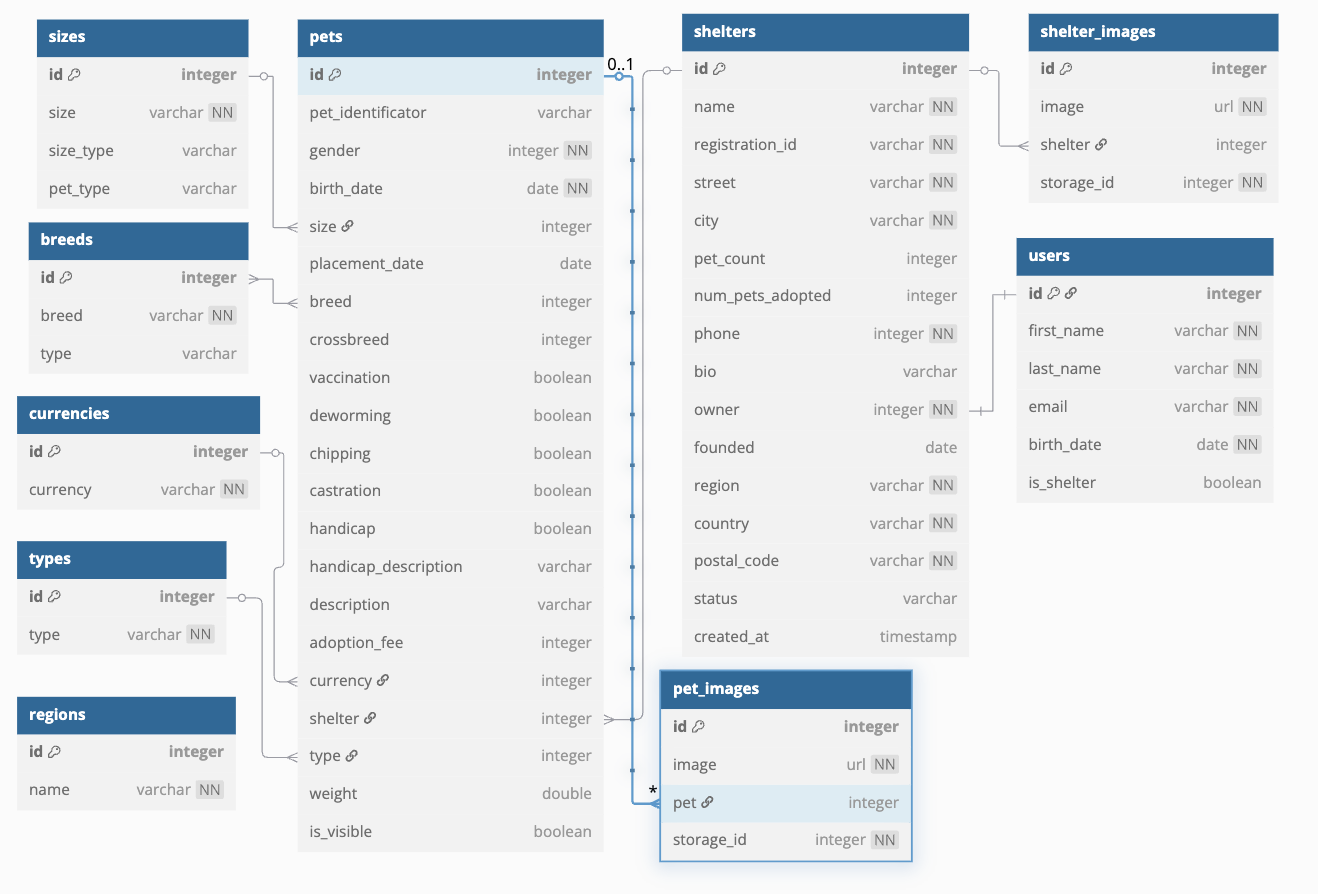
\includegraphics[width=\textwidth]{img-bp/diagram.png} 
    \caption{Databázový návrh}
    \label{fig:diagram}
\end{figure}




\chapter{Instalační příručka}
\label{app:installation}

Instalační příručka obsahuje pokyny pro nasazení a spuštění systému v prostředí React Native s využitím TypeScriptu a Expo.

\section{Nasazení systému}
\label{sec:deployment}

Systém je nasazen ve čtyřech krocích. Prvním z nich je instalace potřebných vývojových nástrojů. Druhým krokem je stažení a nastavení projektu. Třetím krokem je spuštění vývojového prostředí a posledním krokem je vytvoření produkční verze aplikace.

\subsection{Instalace vývojových nástrojů}
\label{subsec:dev-tools}

Pro vývoj aplikace je nutné mít instalované následující nástroje:

\begin{itemize}
    \item IntelliJ IDEA - preferované vývojové prostředí
    \item Node.js (verze 20.0 nebo novější)
    \item Git pro správu verzí kódu
    \item Expo CLI - instalace pomocí příkazu \texttt{npm install -g expo-cli}
\end{itemize}

Pro testování aplikace je doporučeno nainstalovat:

\begin{itemize}
    \item Aplikaci Expo Go na fyzickém zařízení (dostupná v App Store i Google Play)
    \item Android Studio pro spuštění Android emulátoru
    \item Xcode (pouze na macOS) pro spuštění iOS simulátoru
\end{itemize}

\subsection{Stažení a nastavení projektu}
\label{subsec:project-setup}

Pro nastavení projektu je nutné provést následující kroky:

\begin{enumerate}
    \item Stáhnout zdrojové kódy z repozitáře pomocí příkazu:
    
    \texttt{https://github.com/Admiam/Hafu-mobile-app.git}
    
    \item Přejít do adresáře projektu:
    
    \texttt{cd Hafu-mobile-app/Aplikace\_a\_knihovny}
    
    \item Nainstalovat závislosti projektu:
    
    \texttt{npm install}
    
    \item Vytvořit konfigurační soubor \texttt{.env} s následujícími proměnnými:
    \begin{itemize}
        \item \texttt{APPWRITE\_ENDPOINT} - URL adresa Appwrite serveru
        \item \texttt{APPWRITE\_PROJECT\_ID} - ID projektu v Appwrite
        \item \texttt{APPWRITE\_DATABASE\_ID} - ID databáze v Appwrite
        \item \texttt{APPWRITE\_STORAGE\_ID} - ID úložiště pro soubory v Appwrite
    \end{itemize}
\end{enumerate}

\subsection{Spuštění vývojového prostředí}
\label{subsec:dev-environment}

Pro spuštění aplikace ve vývojovém režimu je nutné provést následující kroky:

\begin{enumerate}
    \item Otevřít projekt v IntelliJ IDEA
    \item Spustit Metro bundler příkazem v terminálu:
    
    \texttt{npm start}
    
    \item Po spuštění se v terminálu zobrazí QR kód, který lze naskenovat pomocí aplikace Expo Go na fyzickém zařízení
    \item Alternativně lze spustit aplikaci na emulátoru stisknutím klávesy \button{a} pro Android nebo \button{i} pro iOS v terminálu s běžícím Metro bundlerem
\end{enumerate}

Metro bundler nabízí režim hot-reload, který umožňuje okamžité promítnutí změn v kódu do běžící aplikace bez nutnosti manuálního restartování.

\subsection{Vytvoření produkční verze}
\label{subsec:production-build}

Pro vytvoření produkční verze aplikace je doporučeno použít službu EAS (Expo Application Services):

\begin{enumerate}
    \item Instalace EAS CLI:
    
    \texttt{npm install -g eas-cli}
    
    \item Přihlášení k Expo účtu:
    
    \texttt{eas login}
    
    \item Konfigurace EAS pro projekt:
    
    \texttt{eas build:configure}
    
    \item Úprava souboru \texttt{eas.json} dle potřeb projektu
    \item Vytvoření produkčního buildu pro Android:
    
    \texttt{eas build -p android --profile production}
    
    \item Vytvoření produkčního buildu pro iOS (pouze na macOS):
    
    \texttt{eas build -p ios --profile production}
\end{enumerate}

Vytvořené produkční buildy lze stáhnout z Expo dashboardu nebo přímo distribuovat do obchodů s aplikacemi (Google Play Store, App Store).

\section{Konfigurace Appwrite backendu}
\label{sec:appwrite-config}

Aplikace využívá jako backend službu Appwrite, kterou je nutné před použitím aplikace správně nakonfigurovat.

\subsection{Vytvoření Appwrite projektu}
\label{subsec:appwrite-project}

Pro vytvoření Appwrite projektu je nutné:

\begin{enumerate}
    \item Vytvořit účet na \texttt{https://cloud.appwrite.io} nebo nainstalovat self-hosted verzi Appwrite
    \item Vytvořit nový projekt s libovolným názvem
    \item Zaznamenat si Project ID, které bude potřeba pro konfiguraci klienta
    \item V sekci \texttt{Platforms} přidat novou platformu typu \texttt{Flutter App} (funguje i pro React Native) a nastavit název balíčku aplikace (např. \texttt{com.example.myapp})
\end{enumerate}

\subsection{Nastavení databáze a kolekcí}
\label{subsec:database-collections}

V Appwrite je nutné vytvořit databázi a kolekce pro ukládání dat:

\begin{enumerate}
    \item V sekci \texttt{Databases} vytvořit novou databázi
    \item Vytvořit následující kolekce:
    \begin{itemize}
        \item \texttt{users} - pro ukládání dat o uživatelích
        \item \texttt{shelters} - pro ukládání dat o útulcích
        \item \texttt{pets} - pro ukládání dat o zvířatech
        \item \texttt{visits} - pro ukládání záznamů o návštěvách zvířat
    \end{itemize}
    \item Pro každou kolekci nastavit atributy podle datového modelu popsaného v sekci \ref{sec:datovy_model}
    \item Nastavit správná oprávnění pro každou kolekci:
    \begin{itemize}
        \item Read: \texttt{role:all} (pro veřejné čtení)
        \item Create/Update/Delete: \texttt{role:member} (pouze pro přihlášené uživatele)
    \end{itemize}
\end{enumerate}

\subsection{Nastavení úložiště}
\label{subsec:storage-setup}

Pro ukládání obrázků je nutné nastavit úložiště:

\begin{enumerate}
    \item V sekci \texttt{Storage} vytvořit dva buckety:
    \begin{itemize}
        \item \texttt{pet\_images} - pro ukládání fotografií zvířat
        \item \texttt{shelter\_images} - pro ukládání fotografií útulků
    \end{itemize}
    \item Pro každý bucket nastavit maximální velikost souboru na 5 MB
    \item Povolit formáty souborů: \texttt{.jpg}, \texttt{.png}
    \item Nastavit oprávnění:
    \begin{itemize}
        \item Read: \texttt{role:all} (pro veřejné čtení)
        \item Create/Update/Delete: \texttt{role:member} (pouze pro přihlášené uživatele)
    \end{itemize}
\end{enumerate}

\subsection{Nastavení autentizace}
\label{subsec:auth-setup}

Pro správné fungování přihlašování je nutné:

\begin{enumerate}
    \item V sekci \texttt{Auth} nastavit metody přihlašování:
    \begin{itemize}
        \item Povolit přihlašování pomocí e-mailu a hesla
        \item Nastavit minimální délku hesla a další požadavky na bezpečnost
    \end{itemize}
    
\end{enumerate}

Po dokončení všech výše uvedených kroků je systém připraven k použití. V mobilní aplikaci stačí nastavit správné hodnoty proměnných prostředí v souboru \texttt{.env} a aplikace se připojí k vytvořenému Appwrite backendu.






\chapter{Uživatelská příručka}
\label{app:user-manual}

Tato uživatelská příručka obsahuje podrobné informace o~konfiguraci a~používání mobilní aplikace pro útulky a~zájemce o~adopci zvířat. Aplikace byla vyvinuta s~využitím technologií \product{React Native}, \product{TypeScript} a~\product{Expo}.

\section{Úvod}
\label{sec:introduction}

Mobilní aplikace slouží jako platforma pro propojení zájemců o~adopci zvířat s~útulky. Aplikace nabízí dvě hlavní role uživatelů:

\begin{itemize}
    \item \textbf{Běžný uživatel} - zájemce o~adopci, který může procházet katalog zvířat, vyhledávat podle různých kritérií, označovat oblíbená zvířata a~kontaktovat útulky
    \item \textbf{Útulek} - organizace, která může spravovat svůj profil, přidávat, upravovat a~odstraňovat záznamy o~zvířatech k~adopci
\end{itemize}

Tato příručka obsahuje kompletní pokyny pro obě uživatelské role.


\section{Vytvoření účtu a~přihlášení}
\label{sec:account-management}

\subsection*{Registrace nového uživatele}

Pro vytvoření účtu běžného uživatele postupujte následovně:

\begin{enumerate}
    \item Na úvodní obrazovce aplikace (viz obrázek \ref{fig:first-page-uz}) zvolte tlačítko\\ \button{PŘIHLÁSIT SE JAKO UŽIVATEL}
    \item Zadejte svou e-mailovou adresu, která nebyla v aplikaci ještě použita, a~klikněte na tlačítko \button{POTVRDIT}
    \item Vyplňte své jméno a~příjmení a~klikněte na tlačítko \button{POTVRDIT}
    \item Zadejte datum narození a~klikněte na tlačítko \button{POTVRDIT}
    \item Vytvořte si heslo (minimálně 8 znaků, obsahující velká a~malá písmena, číslice a~speciální znaky) a~potvrďte jej opětovným zadáním
    \item Klikněte na tlačítko \button{POTVRDIT} pro dokončení registrace
\end{enumerate}

\subsection*{Registrace nového útulku}

Pro vytvoření účtu útulku postupujte následovně:

\begin{enumerate}
    \item Na úvodní obrazovce aplikace (viz obrázek \ref{fig:first-page-uz}) zvolte tlačítko\\ \button{PŘIHLÁSIT SE JAKO ÚTULEK}
    \item Pokračujte v registraci jako běžný uživatel

    \item Vyplňte všechny požadované údaje (viz obrázek \ref{fig:register-shelter-uz}):
    \begin{itemize}
        \item Název útulku/organizace
        \item Adresní údaje (ulice, město, PSČ, region)
        \item Kontaktní telefon
        \item Rok založení organizace
        \item Počet zvířat aktuálně v~útulku
        \item Počet uskutečněných adopcí za poslední rok
        \item Popis útulku a~jeho činnosti
        \item Nahrát alespoň jednu fotografii zařízení
    \end{itemize}
    \item Klikněte na tlačítko \button{POTVRDIT} pro dokončení registrace
\end{enumerate}

\subsection*{Přihlášení do aplikace}


\noindent \textbf{Přihlášení pomocí e-mailu a~hesla}:
    \begin{itemize}
        \item Zadejte svou e-mailovou adresu a~heslo
        \item Klikněte na tlačítko \button{PŘIHLÁSIT SE JAKO UŽIVATEL}, nebo \button{PŘIHLÁSIT SE JAKO ÚTULEK}
    \end{itemize}
    
\begin{figure}[h!]
    \centering
    \begin{subfigure}{0.3\textwidth}
        \centering
        
\includegraphics[width=\textwidth]{img-bp/first-screen.png} 
        \caption{Uvítací obrazovka}
        \label{fig:first-page-uz}
    \end{subfigure}
    \hspace{0.05\textwidth}
    \begin{subfigure}{0.3\textwidth}
        \centering
        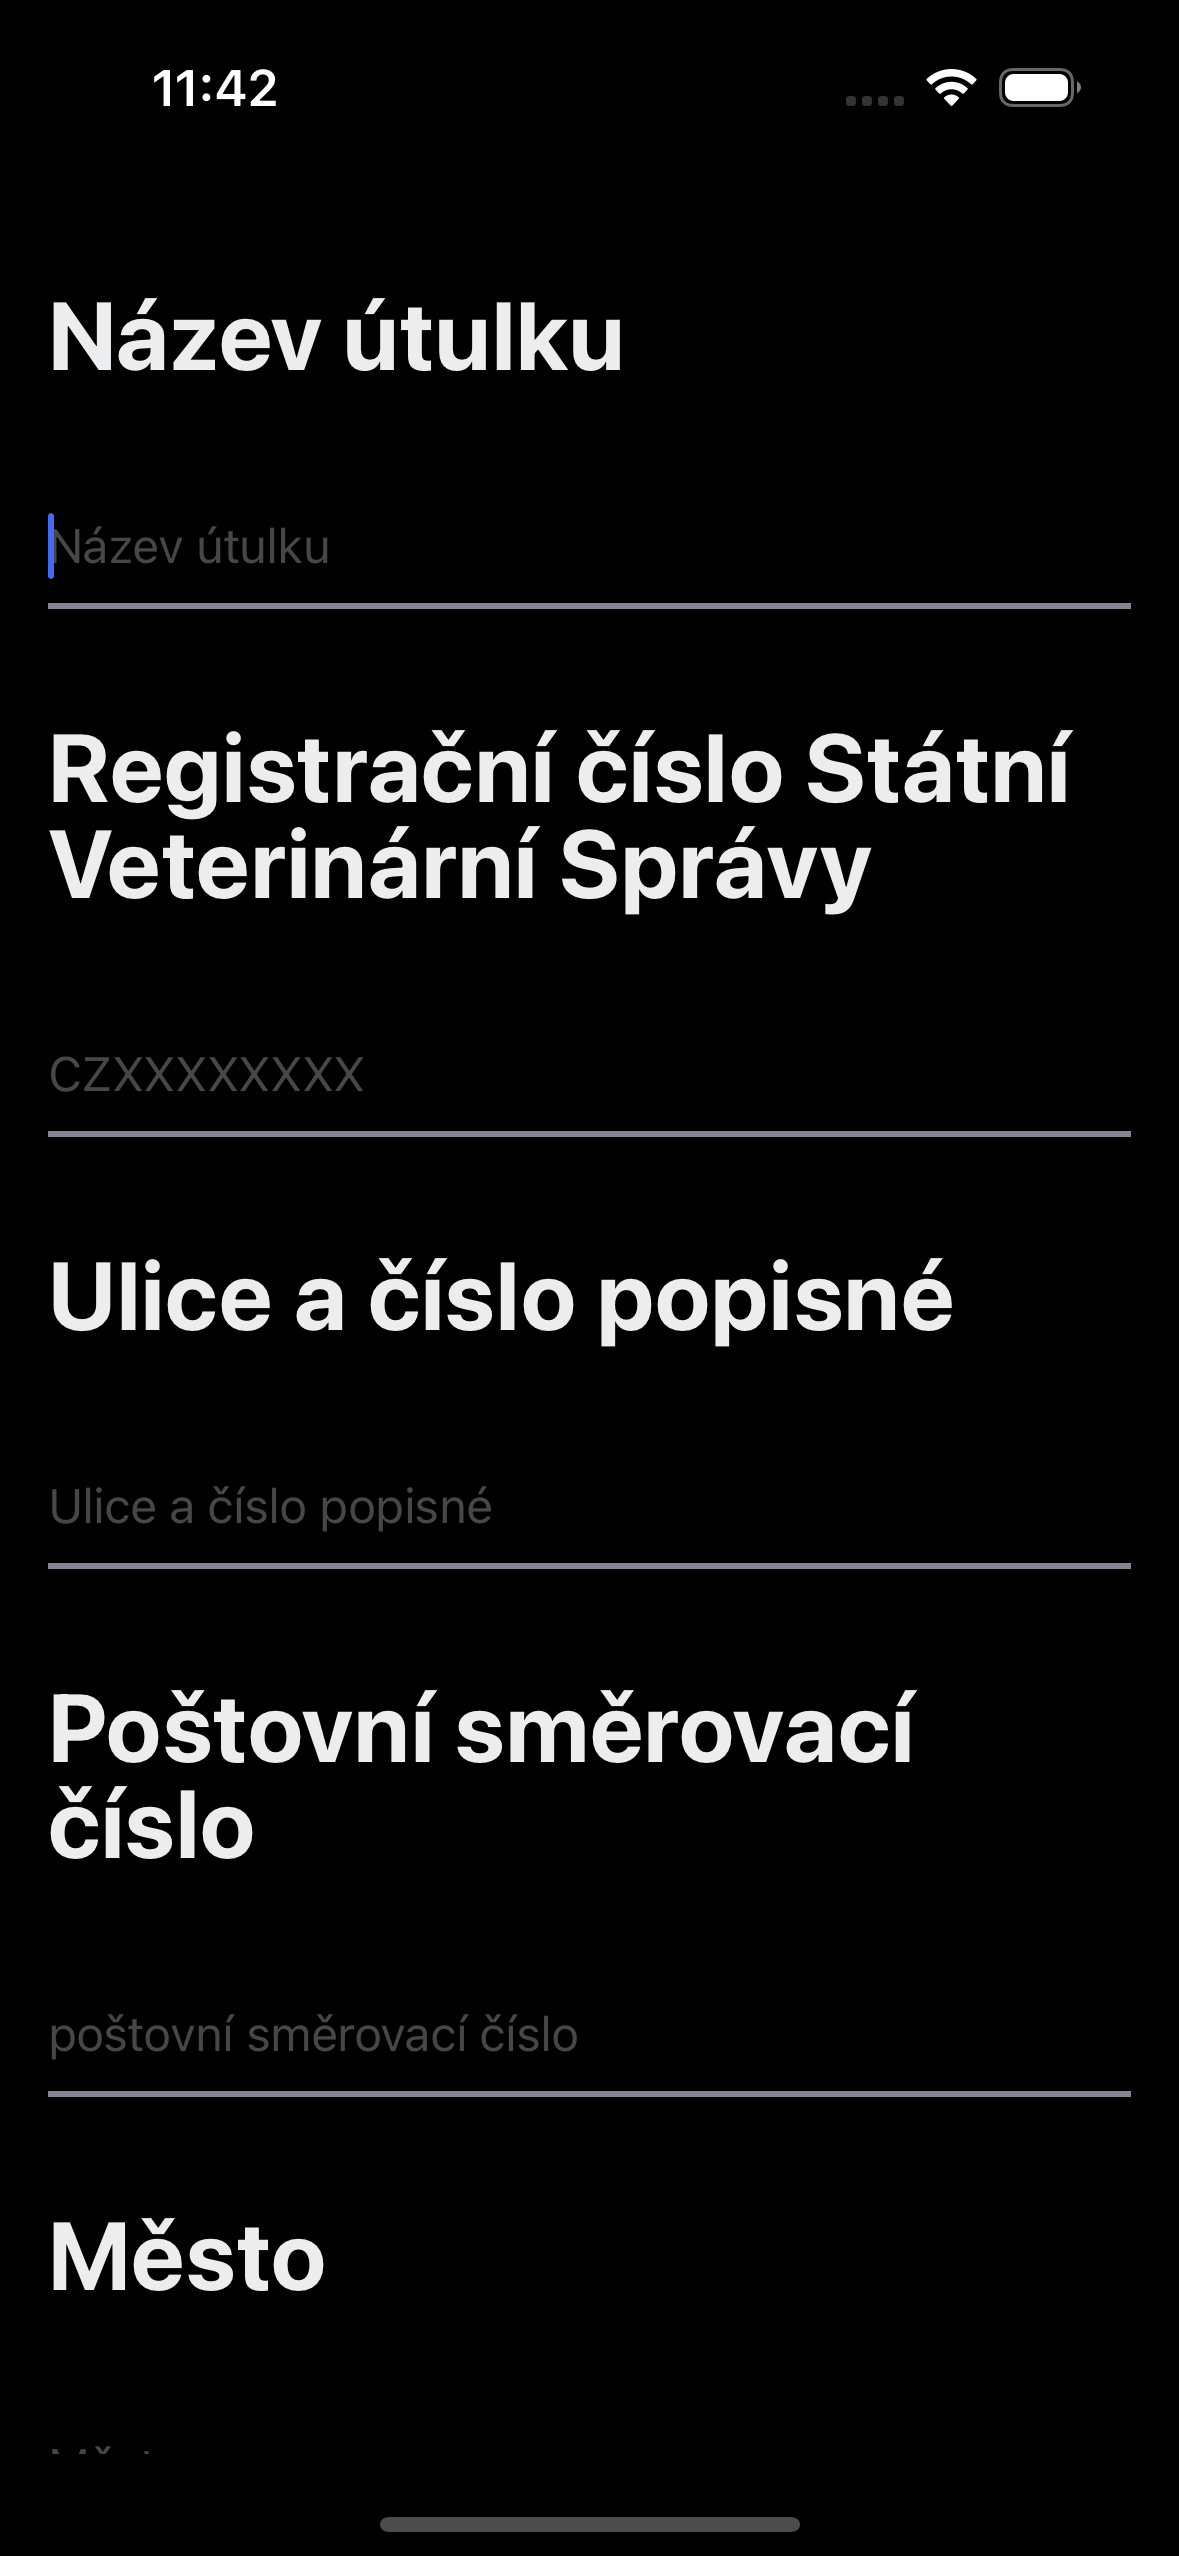
\includegraphics[width=\textwidth]{img-bp/register-shelter.png} 
        \caption{Registrace útulku}
        \label{fig:register-shelter-uz}
    \end{subfigure}
    \caption{Ukázky registrace z aplikace}
    \label{fig:register-uz}
\end{figure}

\break

\section{Uživatelské rozhraní - Běžný uživatel}
\label{sec:ui-regular-user}

Po přihlášení do aplikace jako běžný uživatel se zobrazí hlavní navigační panel v~dolní části obrazovky s~následujícími záložkami:

\begin{itemize}
    \item \textbf{Domů}: Obrazovka s~doporučenými zvířaty ve formátu karet, kterými lze listovat gesty (swipe doprava pro \uv{líbí se}, doleva pro \uv{nelíbí se})
    \item \textbf{Procházet}: Seznam všech dostupných zvířat s~možnostmi filtrování a~řazení
    \item \textbf{Oblíbené}: Seznam zvířat, která jste označili jako oblíbená
    \item \textbf{Profil}: Správa vašeho profilu, historie návštěv a~další nastavení
\end{itemize}

\subsection*{Domovská obrazovka}

Na domovské obrazovce (viz obrázek \ref{fig:home-page-uz}) jsou zobrazeny karty se zvířaty, které můžete:

\begin{itemize}
    \item Přejet prstem doprava pro označení jako oblíbené
    \item Přejet prstem doleva pro přeskočení
    \item Přejet prstem směrem nahoru nebo stisknutím informačního panelu zvířete přejdeme na obrazovku s detailními informacemi o vybraném zvířeti.
\end{itemize}

Každá karta obsahuje základní informace o~zvířeti, jako je jméno, věk, vzdálenost od vaší polohy a~fotografie.

\subsection*{Procházení katalogu zvířat}

V~sekci \textbf{Procházet} (viz obrázek \ref{fig:explore-page-uz}) naleznete následující funkce:

\begin{itemize}
    \item Seznam zvířat ve formě karet s~náhledovými obrázky a~základními informacemi
    \item Vyhledávací pole pro rychlé vyhledávání podle jména zvířete
    \item Tlačítko pro filtrování, které otevře nabídku filtračních možností:
    \begin{itemize}
        \item Typ zvířete (vše, psi, kočky)
        \item Pohlaví (vše, samec, samice)
        \item Věk (maximální věk v~měsících nebo letech)
        \item Zdravotní stav (očkování, odčervení, čipování, kastrace, handicap)
    \end{itemize}
    \item Možnosti řazení seznamu:
    \begin{itemize}
        \item Podle abecedy
        \item Podle vzdálenosti
        \item Podle hodnocení
    \end{itemize}
\end{itemize}

Kliknutím na kartu zvířete se otevře detailní zobrazení s~úplnými informacemi.



\subsection*{Detail zvířete}

Obrazovka s~detailem zvířete (viz obrázek \ref{fig:pet-detail-uz}) obsahuje:

\begin{itemize}
    \item Fotogalerii (případně více fotografií)
    \item Jméno a~typ zvířete
    \item Věk a~pohlaví
    \item Vzdálenost od vaší aktuální polohy
    \item Hodnocení a~komentáře ostatních uživatelů
    \item Podrobný popis zvířete
    \item Zdravotní informace (očkování, odčervení, čipování, kastrace, handicap)
    \item Tlačítko \button{Dozvědět se více} pro přesun na detailní stránku útulku (viz obrázek \ref{fig:shelter-detail-uz})
    \item Tlačítko \button{KONTAKTOVAT ÚTULEK} pro přímé spojení s~útulkem
    \item Ikonu srdce pro přidání/odebrání z~oblíbených
\end{itemize}

\begin{figure}[h!]
    \centering
    \begin{subfigure}{0.3\textwidth}
        \centering
        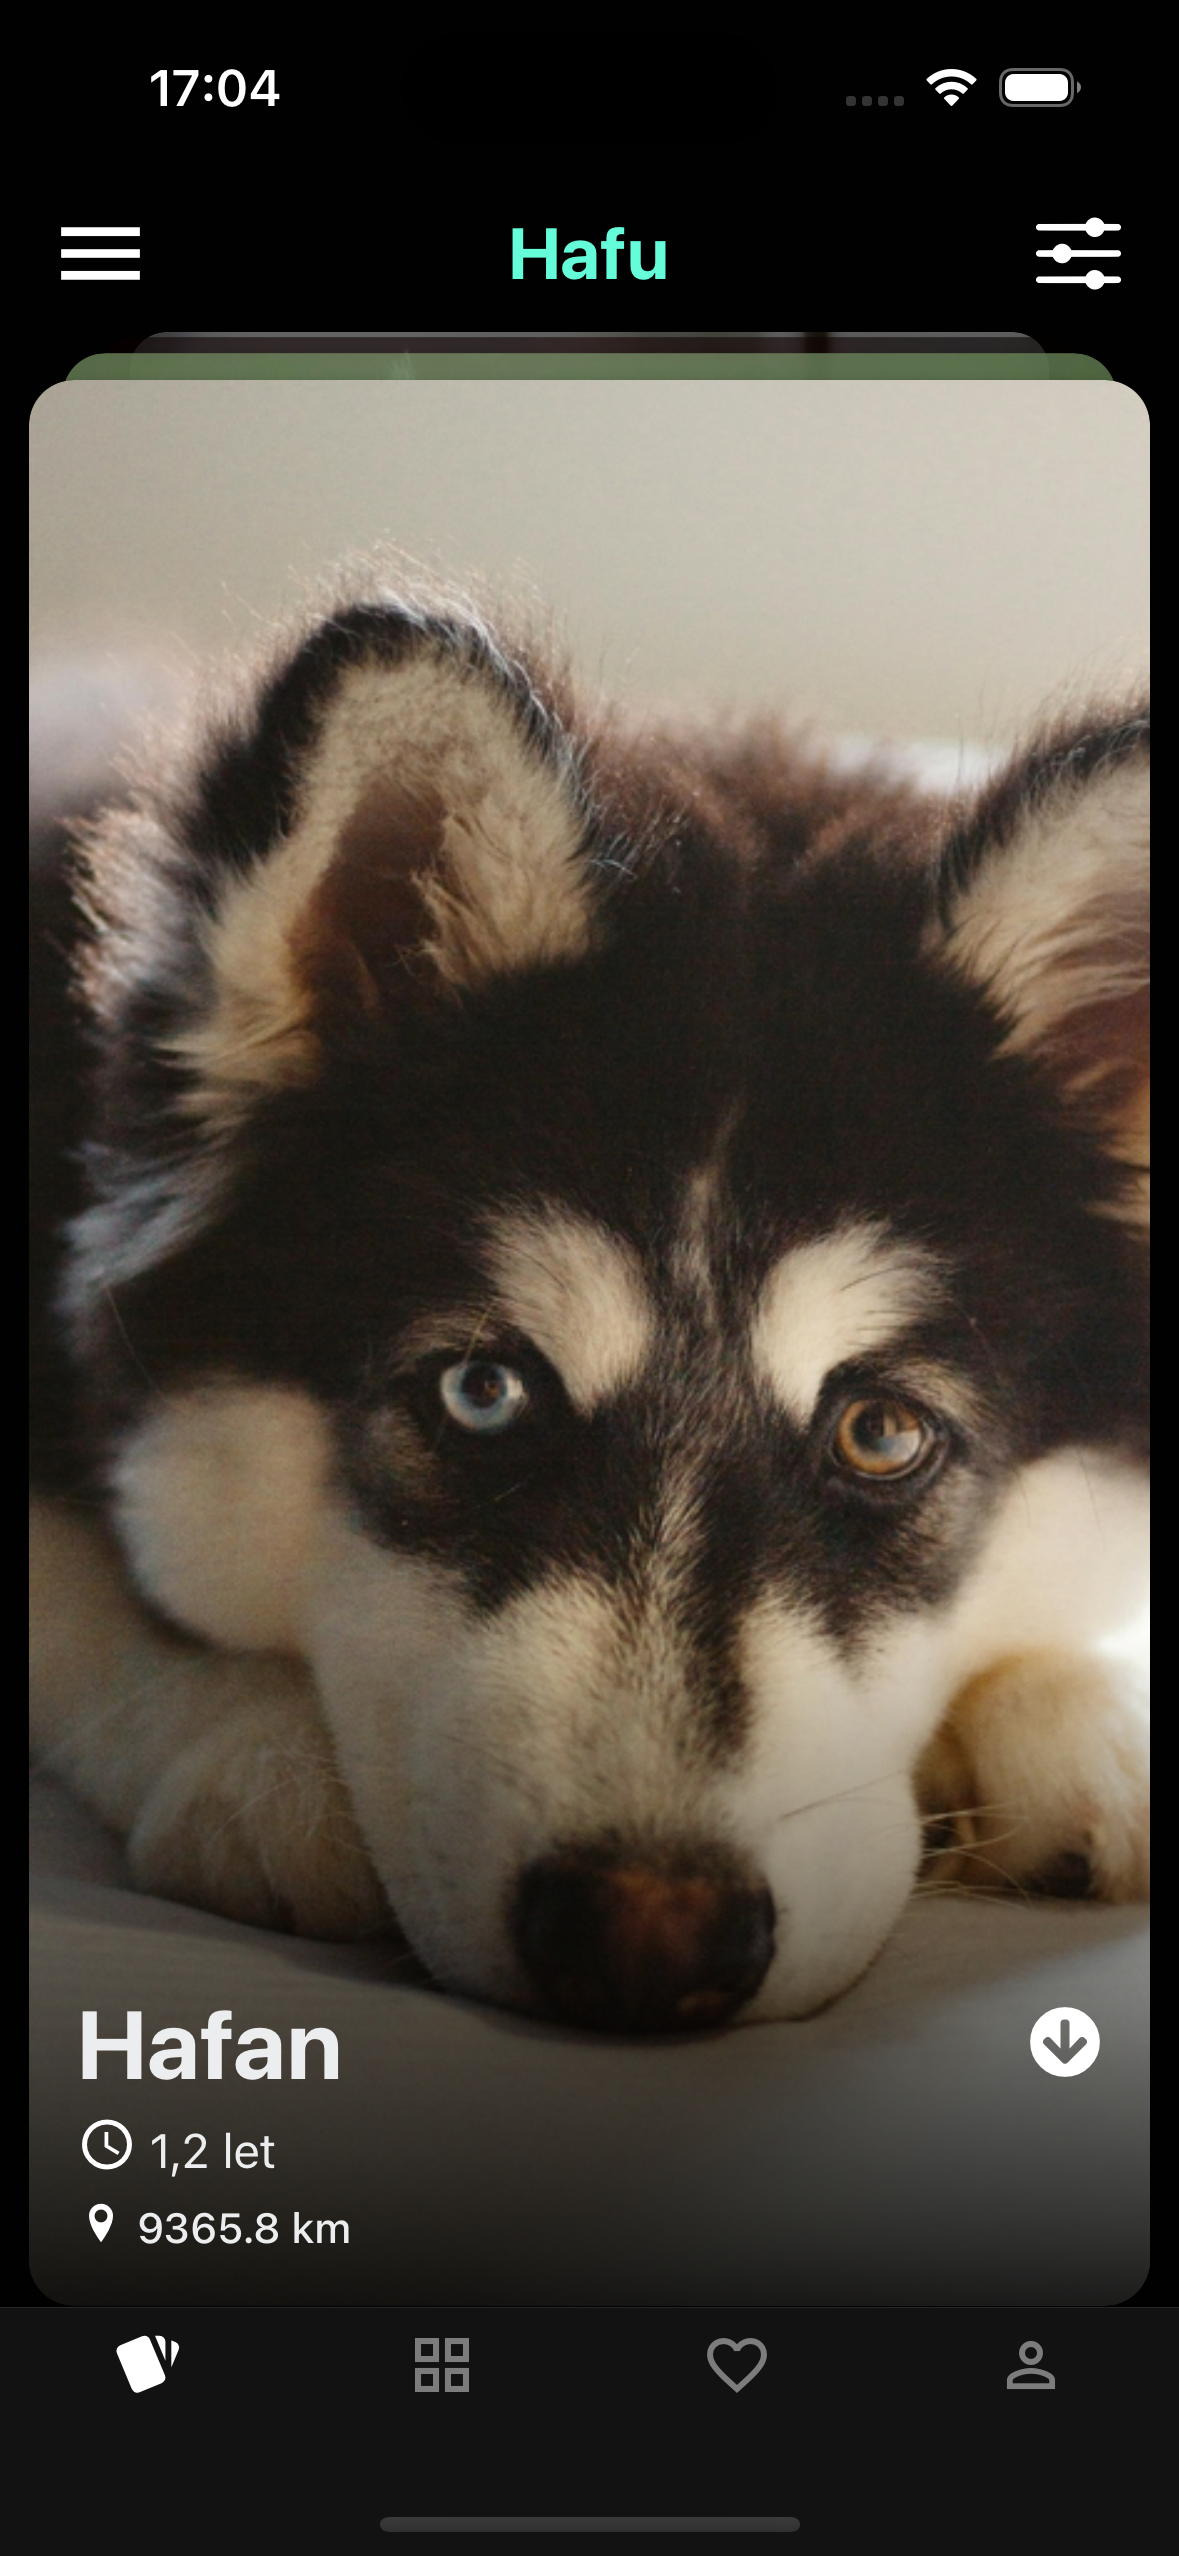
\includegraphics[width=\textwidth]{img-bp/home.png} 
        \caption{Domovská stránka}
        \label{fig:home-page-uz}
    \end{subfigure}
    \hspace{0.03\textwidth}
    \begin{subfigure}{0.3\textwidth}
        \centering
        
\includegraphics[width=\textwidth]{img-bp/explore.png} 
        \caption{Katalog zvířat}
        \label{fig:explore-page-uz}
    \end{subfigure}
    \hspace{0.03\textwidth}
    \begin{subfigure}{0.3\textwidth}
        \centering
        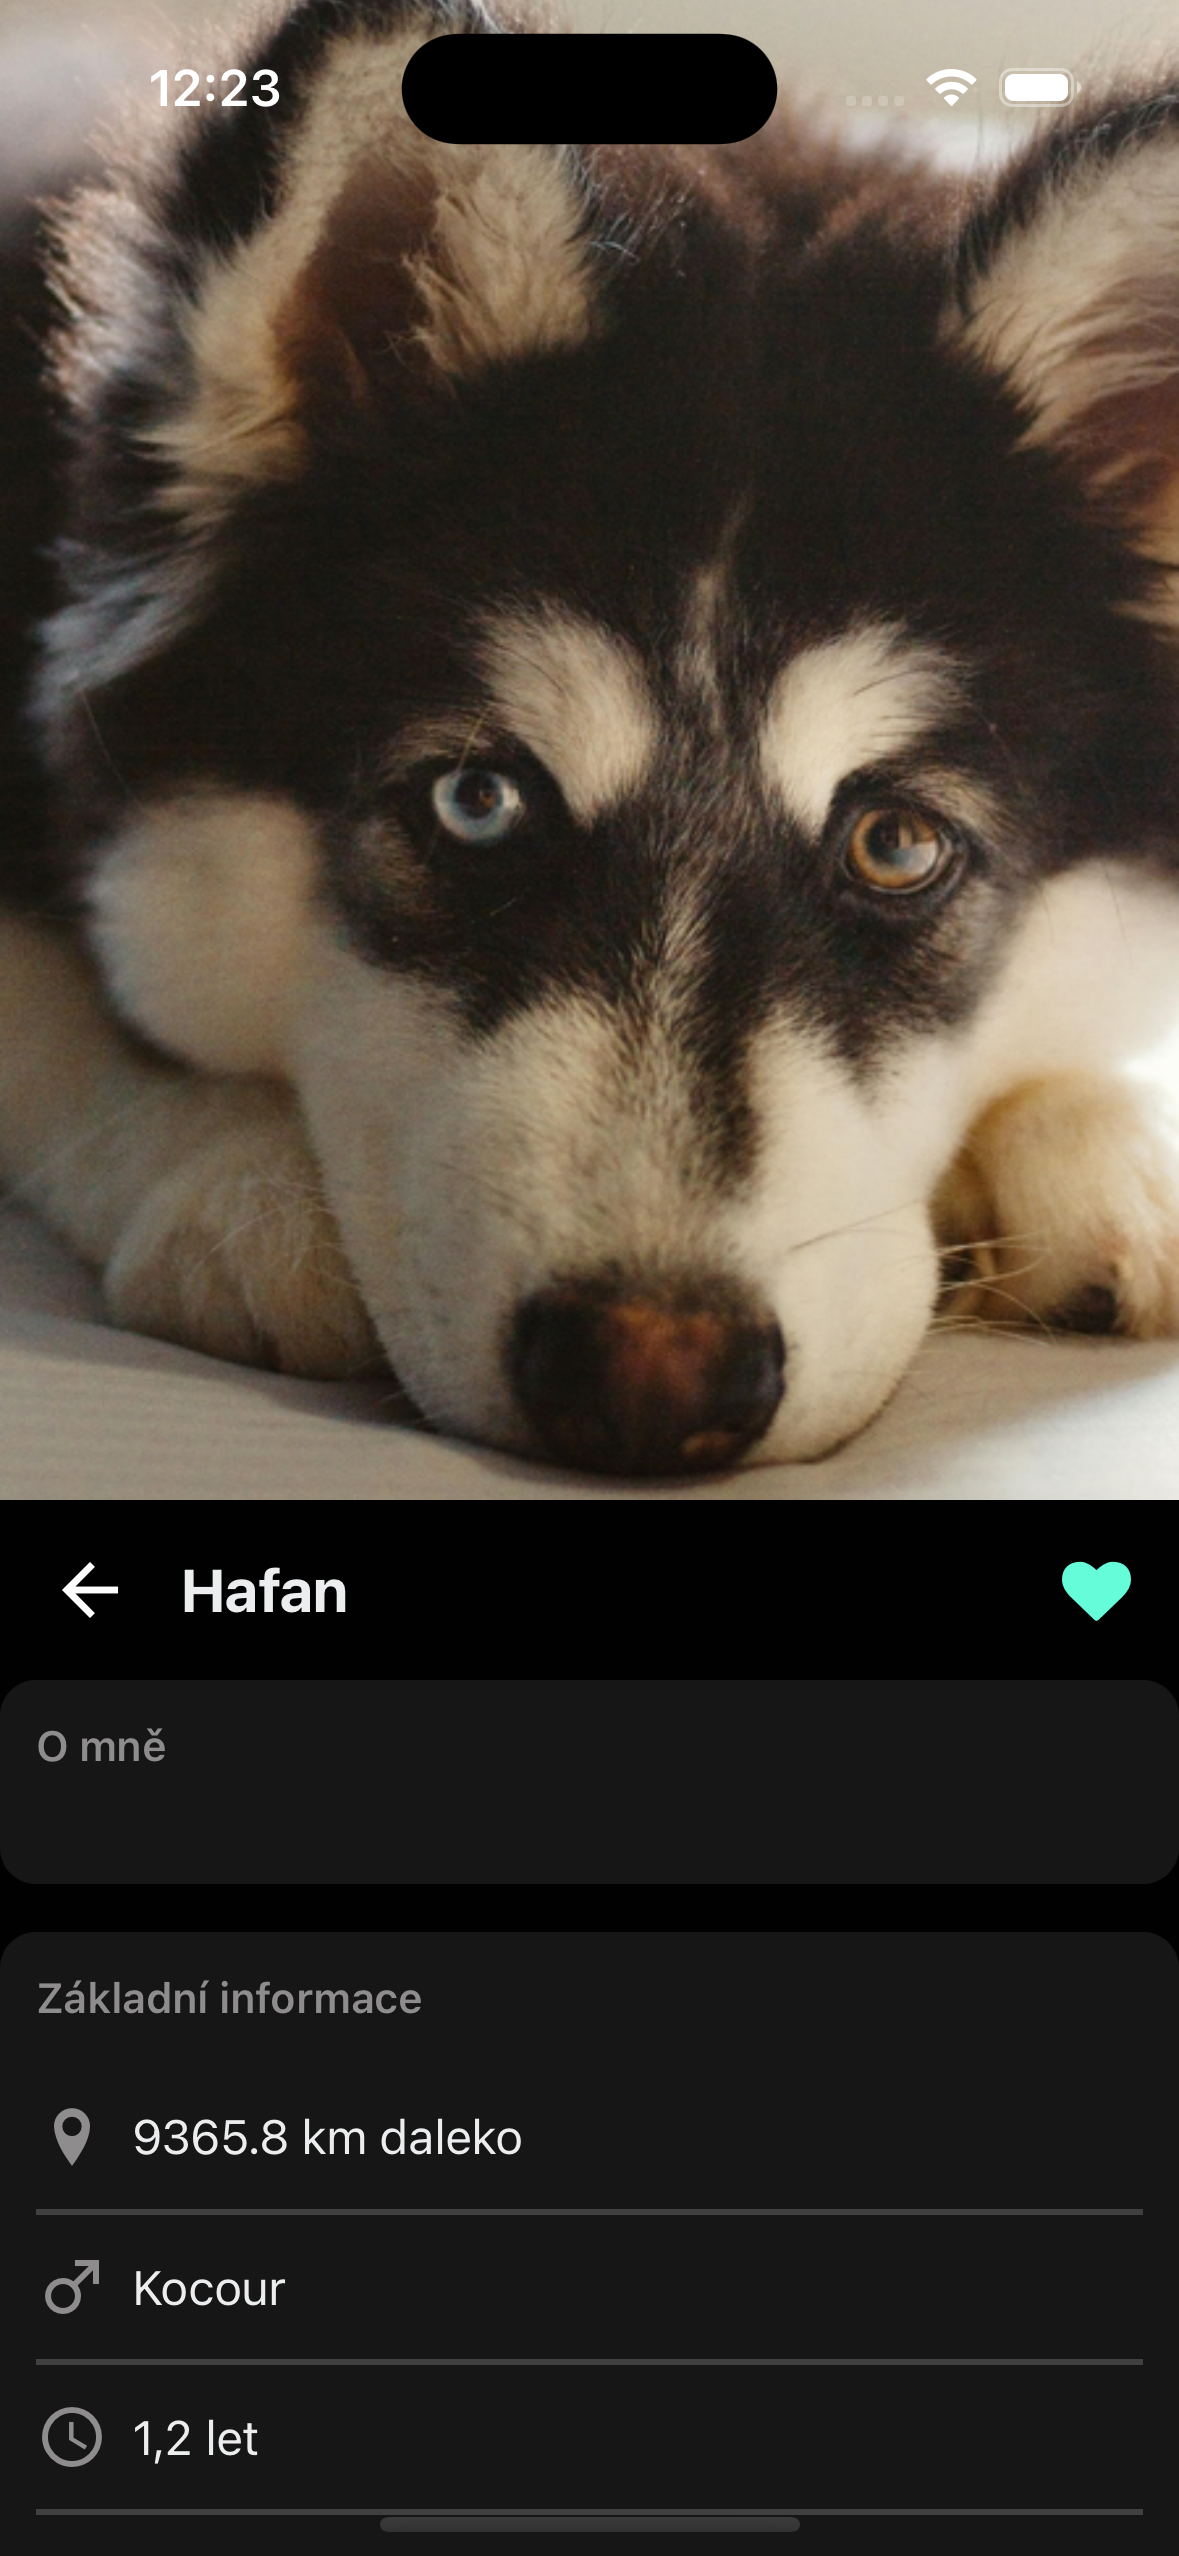
\includegraphics[width=\textwidth]{img-bp/petDetail.png} 
        \caption{Detail zvířete}
        \label{fig:pet-detail-uz}
    \end{subfigure}
    \caption{Ukázky obrazovek z aplikace}
\end{figure}

\subsection*{Sekce Oblíbené}

V~sekci \textbf{Oblíbené} (viz obrázek \ref{fig:match-page-uz}) najdete seznam všech zvířat, která jste označili jako oblíbená. Funkce dostupné v~této sekci:

\begin{itemize}
    \item Seznam oblíbených zvířat s~možností filtrování a~řazení (stejné možnosti jako v~sekci Procházet)
    \item Kliknutím na kartu zvířete se otevře jeho detail
    \item Odstranění z~oblíbených je možné kliknutím na ikonu srdce v~detailu zvířete
    \item Kliknutím na ikonu vlaštovky se otevře kontaktní formulář (viz obrázek \ref{fig:contact-uz})
\end{itemize}

\subsection*{Profil uživatele}

V~sekci \textbf{Profil} (viz obrázek \ref{fig:profile-page-uz}) můžete:

\begin{itemize}
    \item Zobrazit své jméno a~e-mailovou adresu
    \item Upravit své osobní údaje
    \item Stisknutím tlačítka ikony \uv{Změny} se uživatel přesune na obrazovku s formulářem pro úpravu osobních údajů.    
    \item Odhlásit se z~aplikace
    \item Podat žádost pro odstranění účtu
\end{itemize}

\begin{figure}[h!]
    \centering
    \begin{subfigure}{0.3\textwidth}
        \centering
        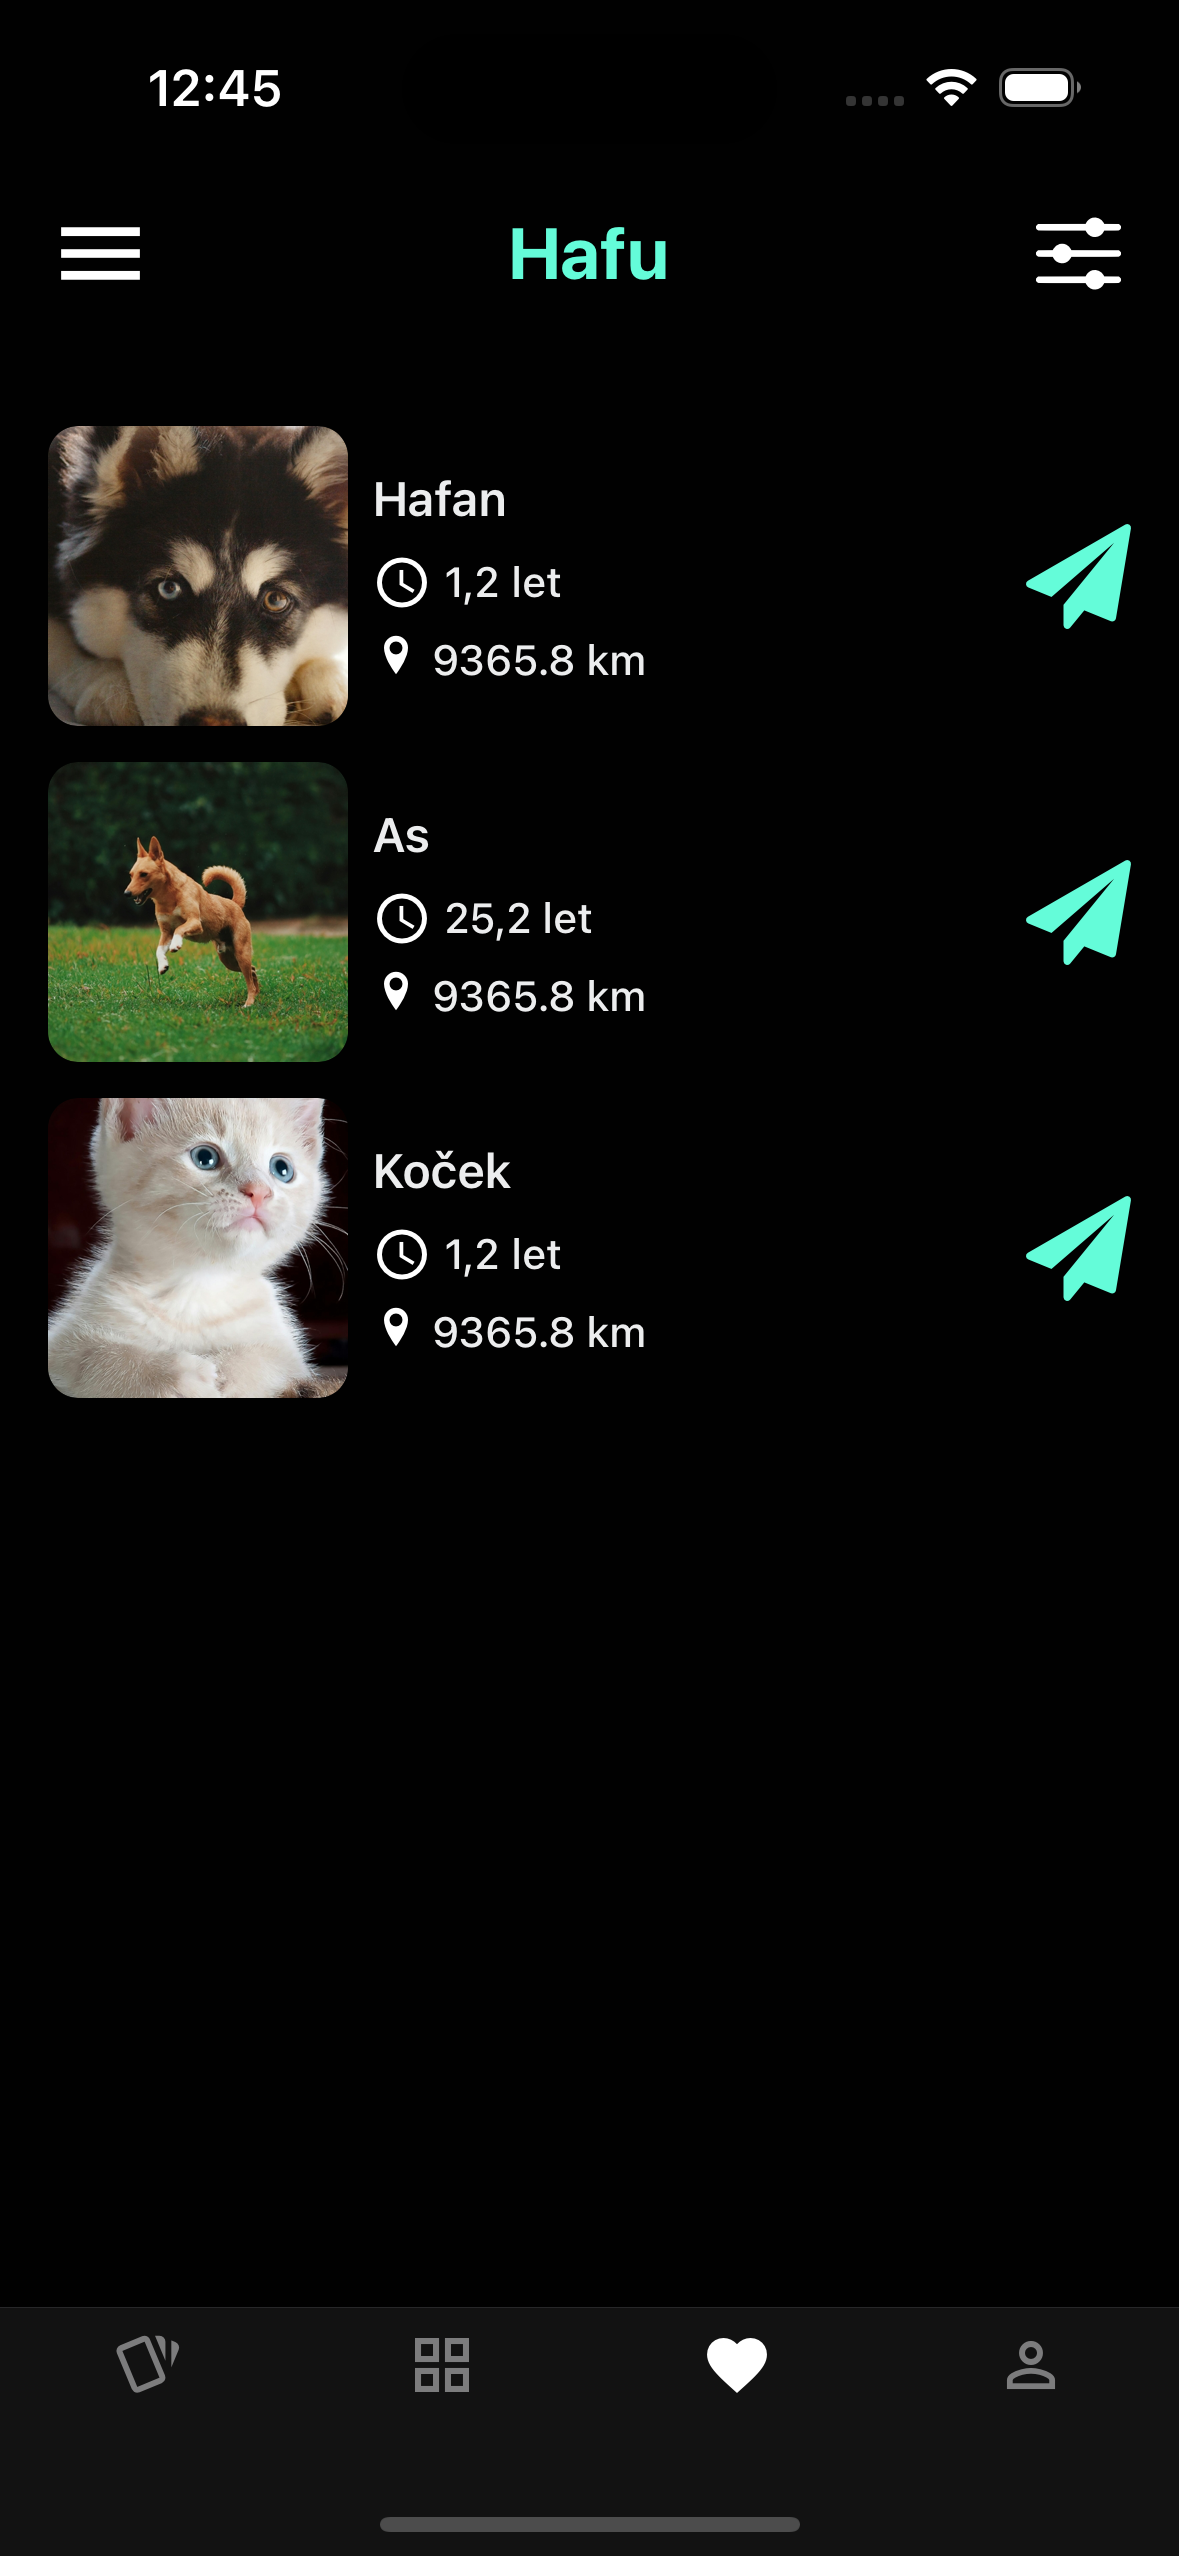
\includegraphics[width=\textwidth]{img-bp/matches.png} 
        \caption{Stránka oblíbené}
        \label{fig:match-page-uz}
    \end{subfigure}
    \hspace{0.03\textwidth}
    \begin{subfigure}{0.3\textwidth}
        \centering
        
\includegraphics[width=\textwidth]{img-bp/account.png} 
        \caption{Stránka profilu}
        \label{fig:profile-page-uz}
    \end{subfigure}
    \hspace{0.03\textwidth}
    \begin{subfigure}{0.3\textwidth}
        \centering
        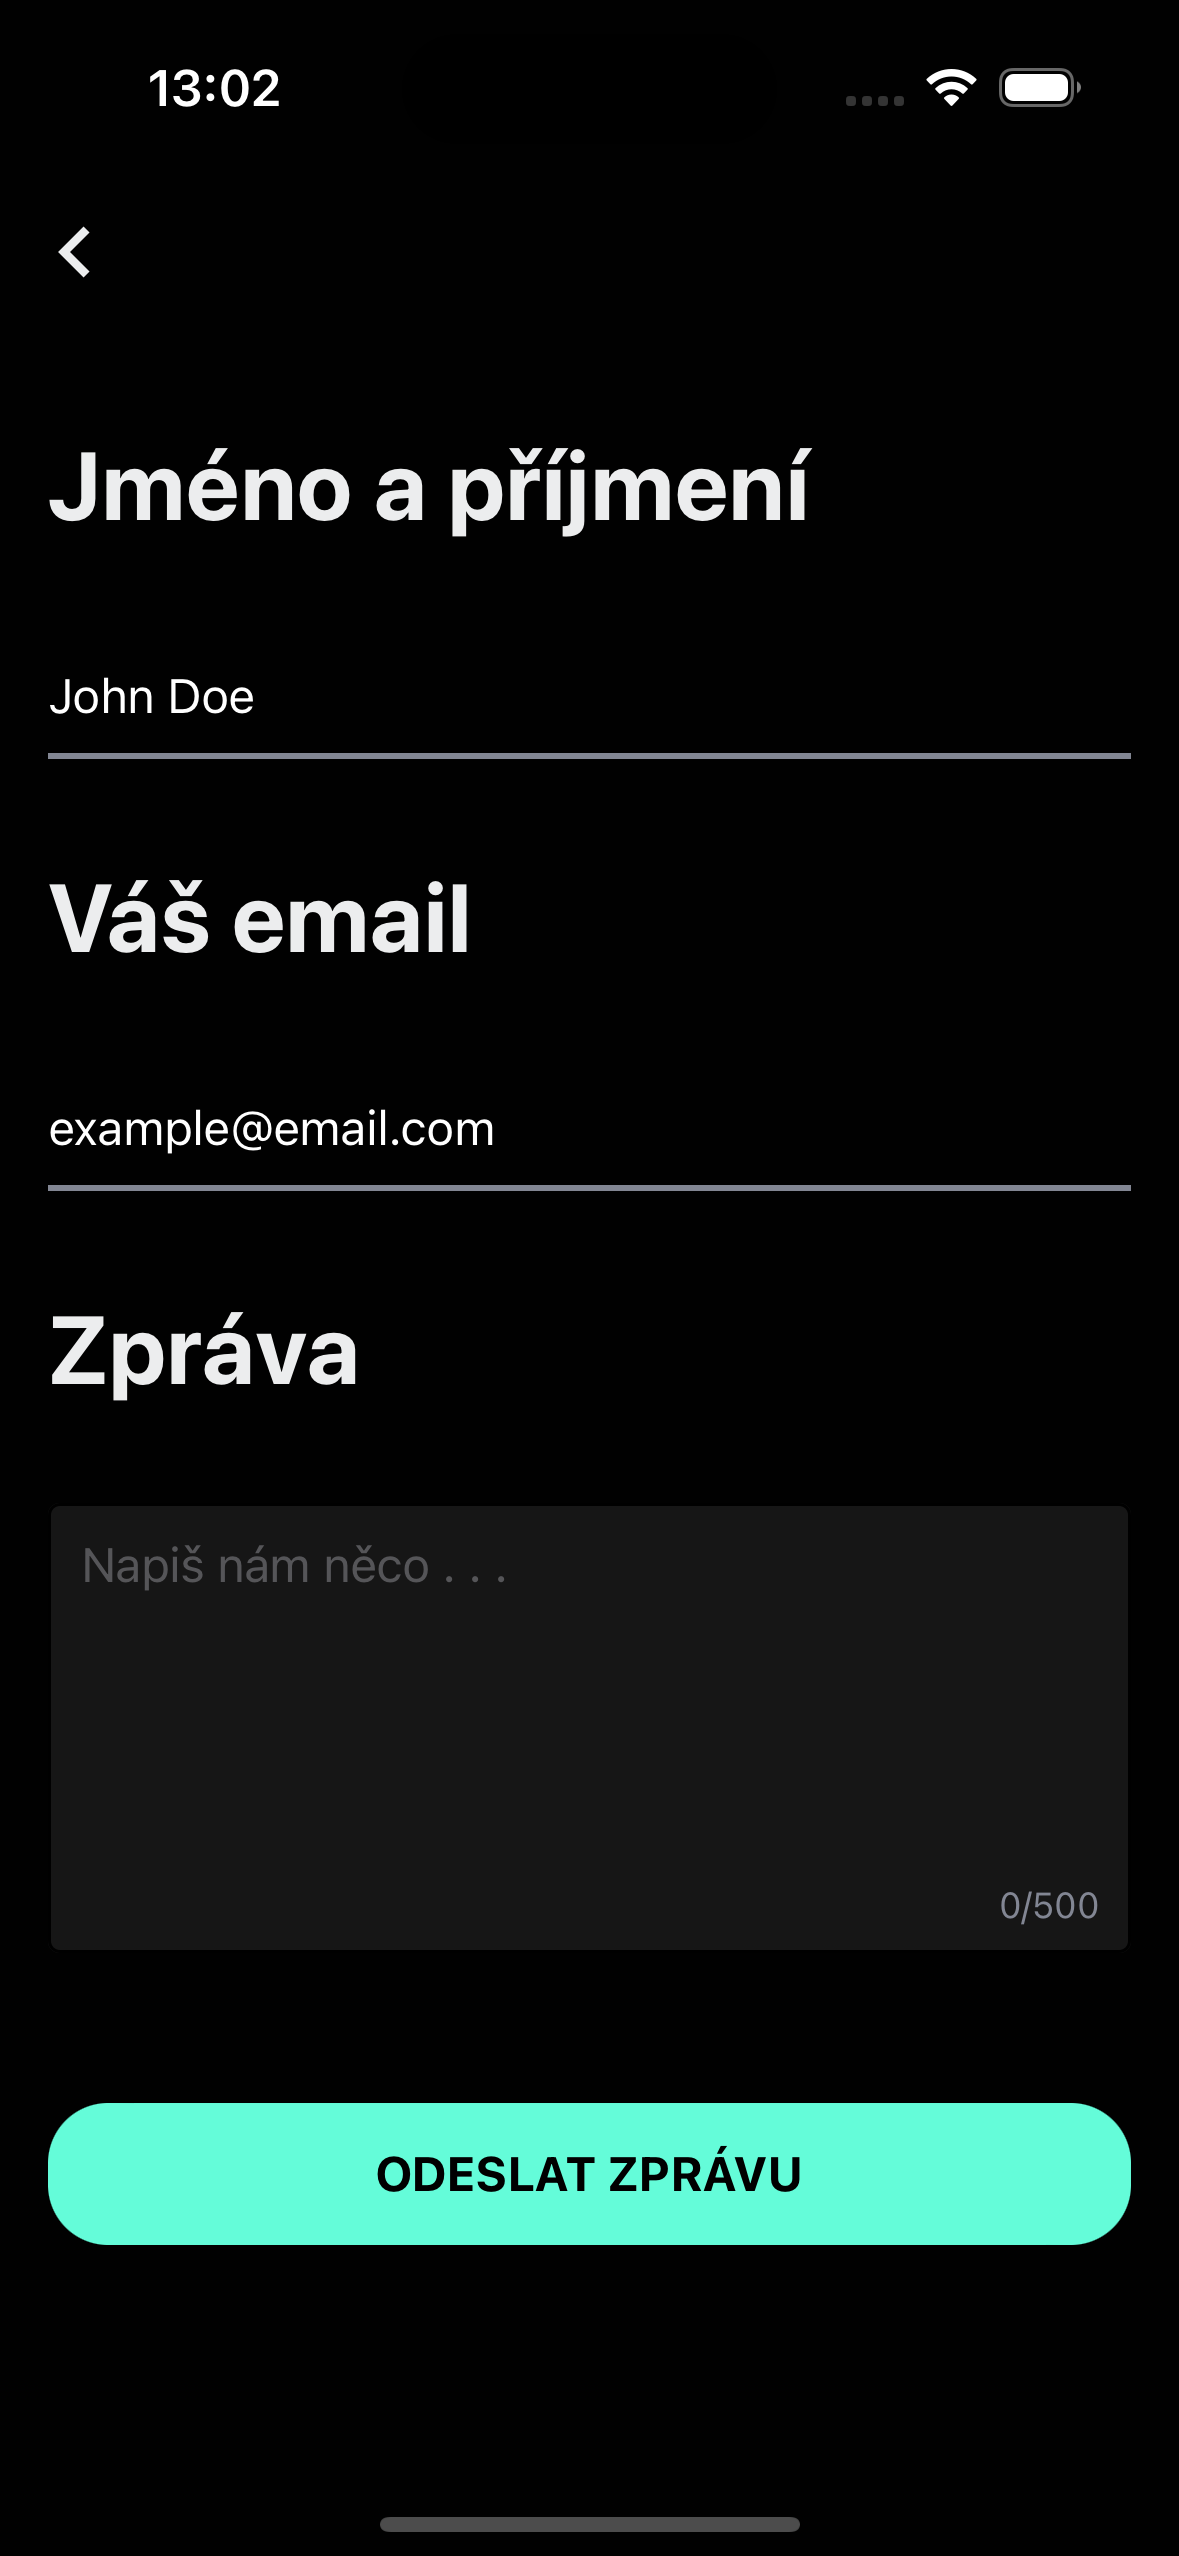
\includegraphics[width=\textwidth]{img-bp/shelterContact.png} 
        \caption{Úprava profilu}
        \label{fig:contact-uz}
    \end{subfigure}
    \caption{Ukázky obrazovek z aplikace}
\end{figure}

\section{Uživatelské rozhraní - Útulek}
\label{sec:ui-shelter}

Po přihlášení do aplikace jako útulek se zobrazí hlavní navigační panel v~dolní části obrazovky a~boční menu pro přístup k~funkcím správy útulku.

\subsection*{Hlavní navigační panel}

Obsahuje stejné záložky jako u~běžného uživatele:

\begin{description}
    \item[\textbf{Domů}] - Přehled aktivity vašeho útulku
    \item[\textbf{Procházet}] - Seznam zvířat v~katalogu
    \item[\textbf{Oblíbené}] - Seznam zvířat, která jste označili jako oblíbená
    \item[\textbf{Profil}] - Správa profilu útulku
\end{description}

\subsection*{Boční menu}

Boční menu obsahuje specializované funkce pro správu útulku:

\begin{description}
    \item[\textbf{Správa zvířat}] - Přidávání, úprava a~mazání zvířat
    \item[\textbf{Profil útulku}] - Úprava informací o~útulku
\end{description}

\subsection*{Správa zvířat}

V~sekci \textbf{Správa zvířat} (viz obrázek \ref{fig:pet-management-uz}) naleznete:

\begin{itemize}
    \item Seznam všech zvířat registrovaných vaším útulkem
    \item Tlačítko \button{PŘIDAT MAZLÍKA} pro přidání nového zvířete
    \item Možnost editace existujících záznamů kliknutím na tlačítko \button{UPRAVIT}
    \item Možnost odstranění záznamu zvířete kliknutím na tlačítko \button{SMAZAT}
\end{itemize}

\subsection*{Přidání nového zvířete}

Pro přidání nového zvířete do databáze (viz obrázek \ref{fig:pet-add-uz}):

\begin{enumerate}
    \item V~sekci Správa zvířat klikněte na tlačítko \button{PŘIDAT MAZLÍKA}
    \item Vyplňte všechny povinné údaje:
    \begin{itemize}
        \item Typ zvířete (pes, kočka)
        \item Jméno zvířete
        \item Pohlaví
        \item Měsíc a~rok narození
        \item Velikost
        \item Váha
        \item Plemeno
        \item Zdravotní stav (zaškrtněte příslušné položky)
        \item Popis zvířete
        \item Adopční poplatek
    \end{itemize}
    \item Nahrajte alespoň jednu fotografii zvířete
    \item Klikněte na tlačítko \button{POTVRDIT} pro uložení záznamu
\end{enumerate}

\important{
Pro úspěšné zaznamenání nového zvířete musí být vyplněna všechna povinná pole a~musí být nahrána alespoň jedna fotografie. Bez splnění těchto podmínek nebude možné formulář odeslat.
}

\subsection*{Úprava profilu útulku}

V~sekci \textbf{Profil útulku} (viz obrázek \ref{fig:shelter-detail-uz}) můžete upravit:

\begin{itemize}
    \item Název organizace
    \item Kontaktní údaje
    \item Adresu
    \item Popis činnosti
    \item Fotografie zařízení
    \item Další statistické údaje (počet zvířat, počet adopcí)
\end{itemize}

Pro uložení změn klikněte na tlačítko \button{ULOŽIT ZMĚNY}.
\begin{figure}[h!]
    \centering
    \begin{subfigure}{0.3\textwidth}
        \centering
        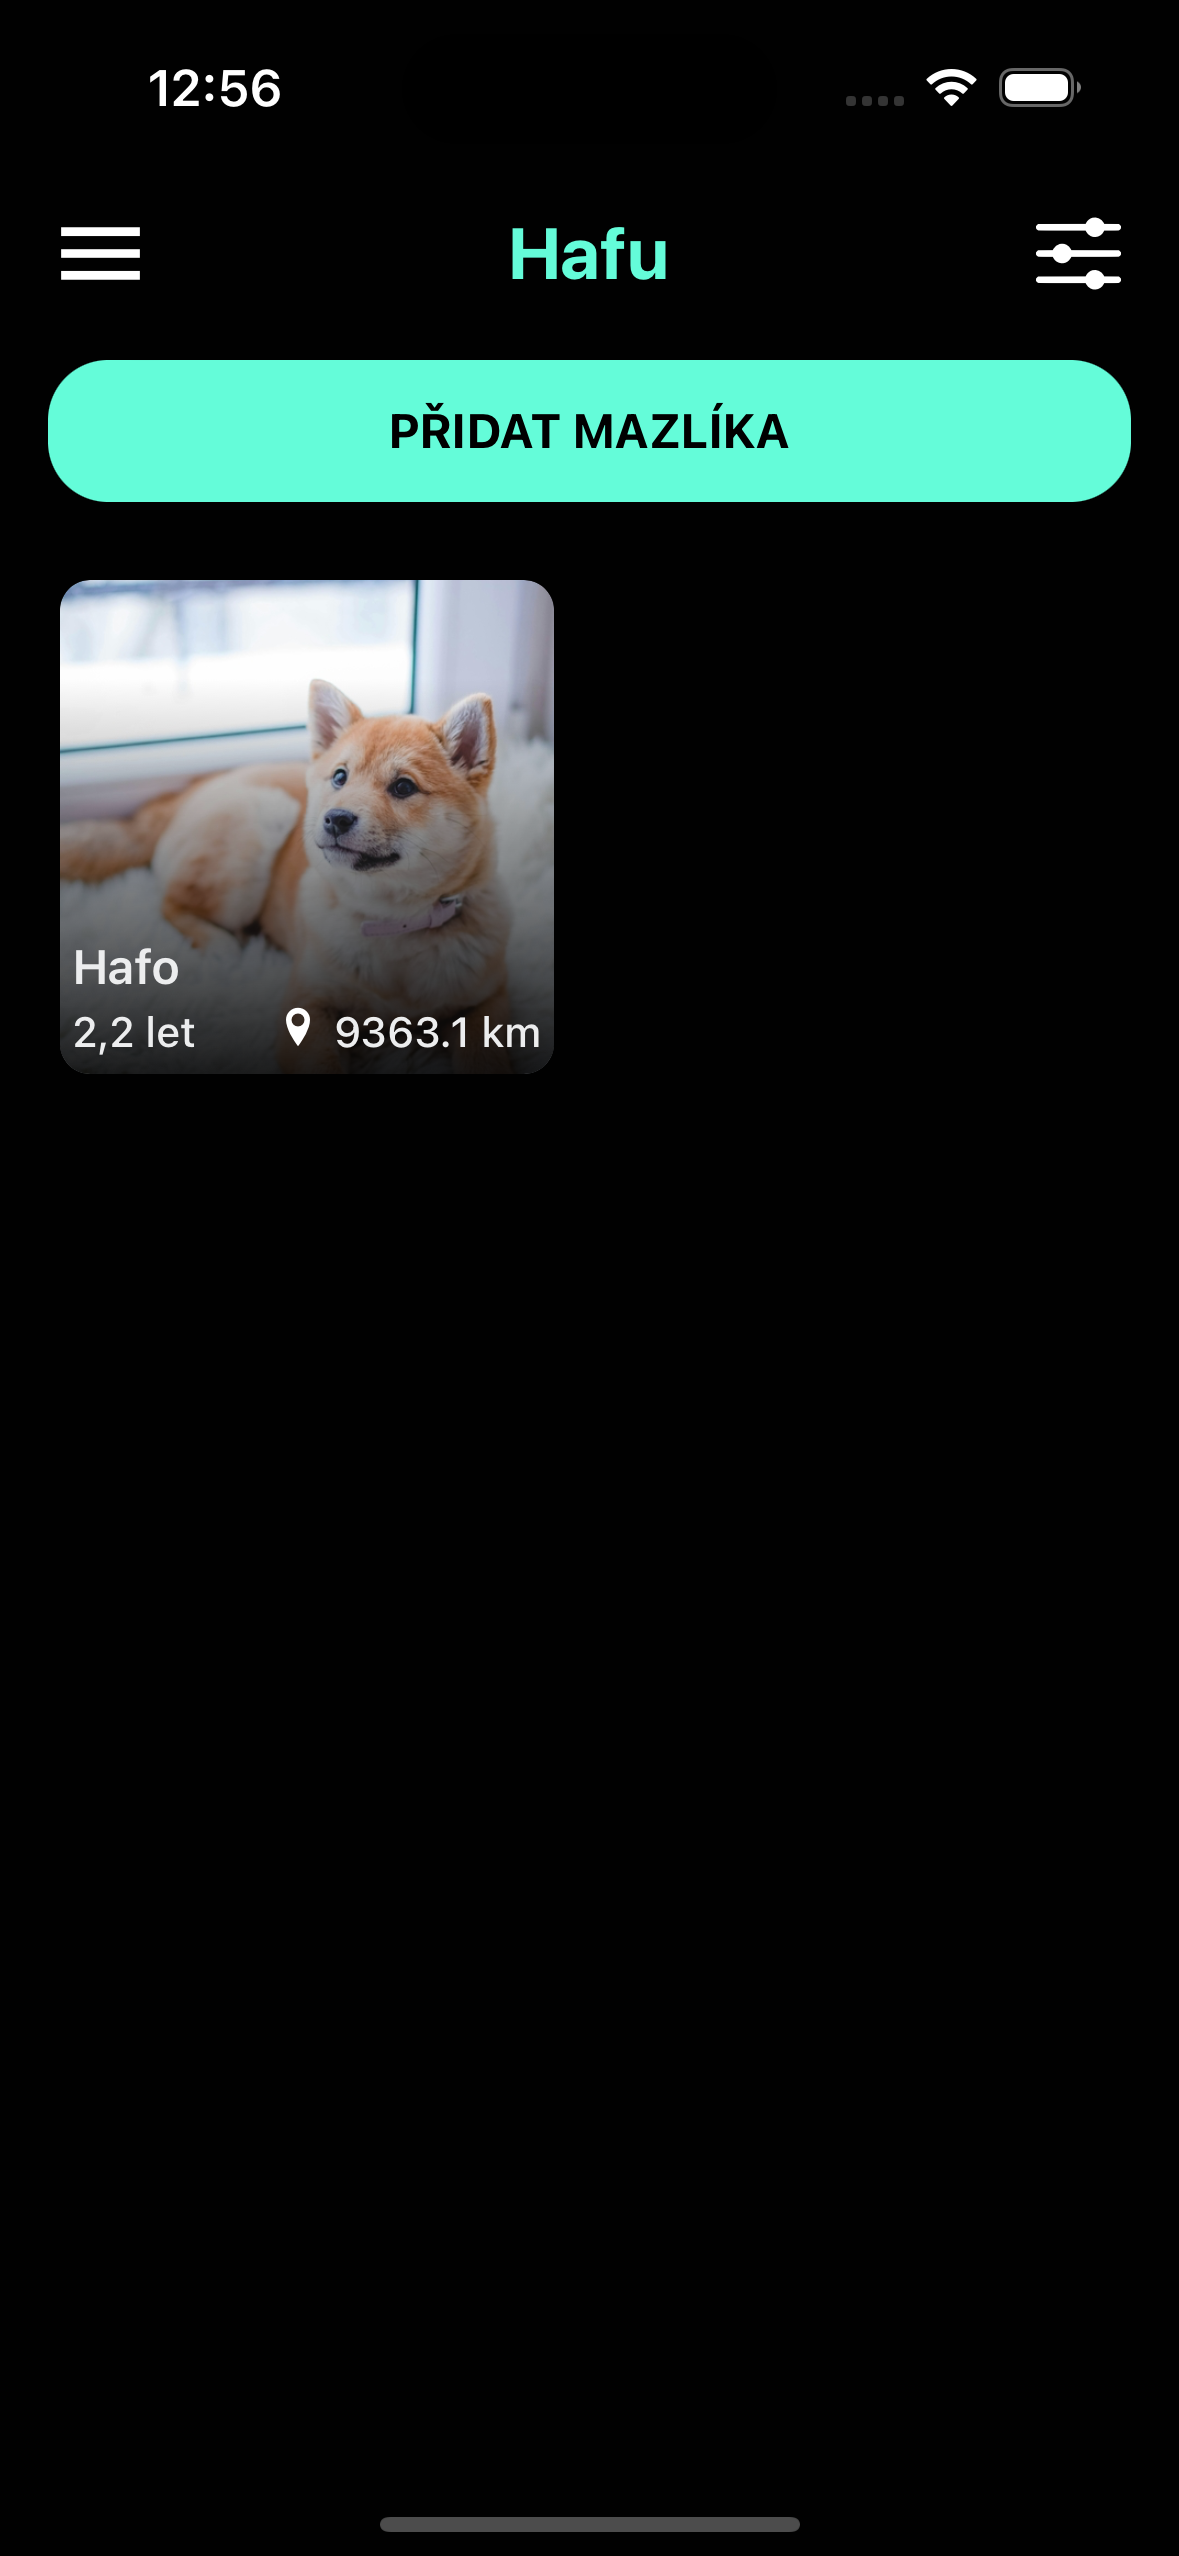
\includegraphics[width=\textwidth]{img-bp/petManagement.png} 
        \caption{Správa zvířat}
        \label{fig:pet-management-uz}
    \end{subfigure}
    \hspace{0.03\textwidth}
    \begin{subfigure}{0.3\textwidth}
        \centering
        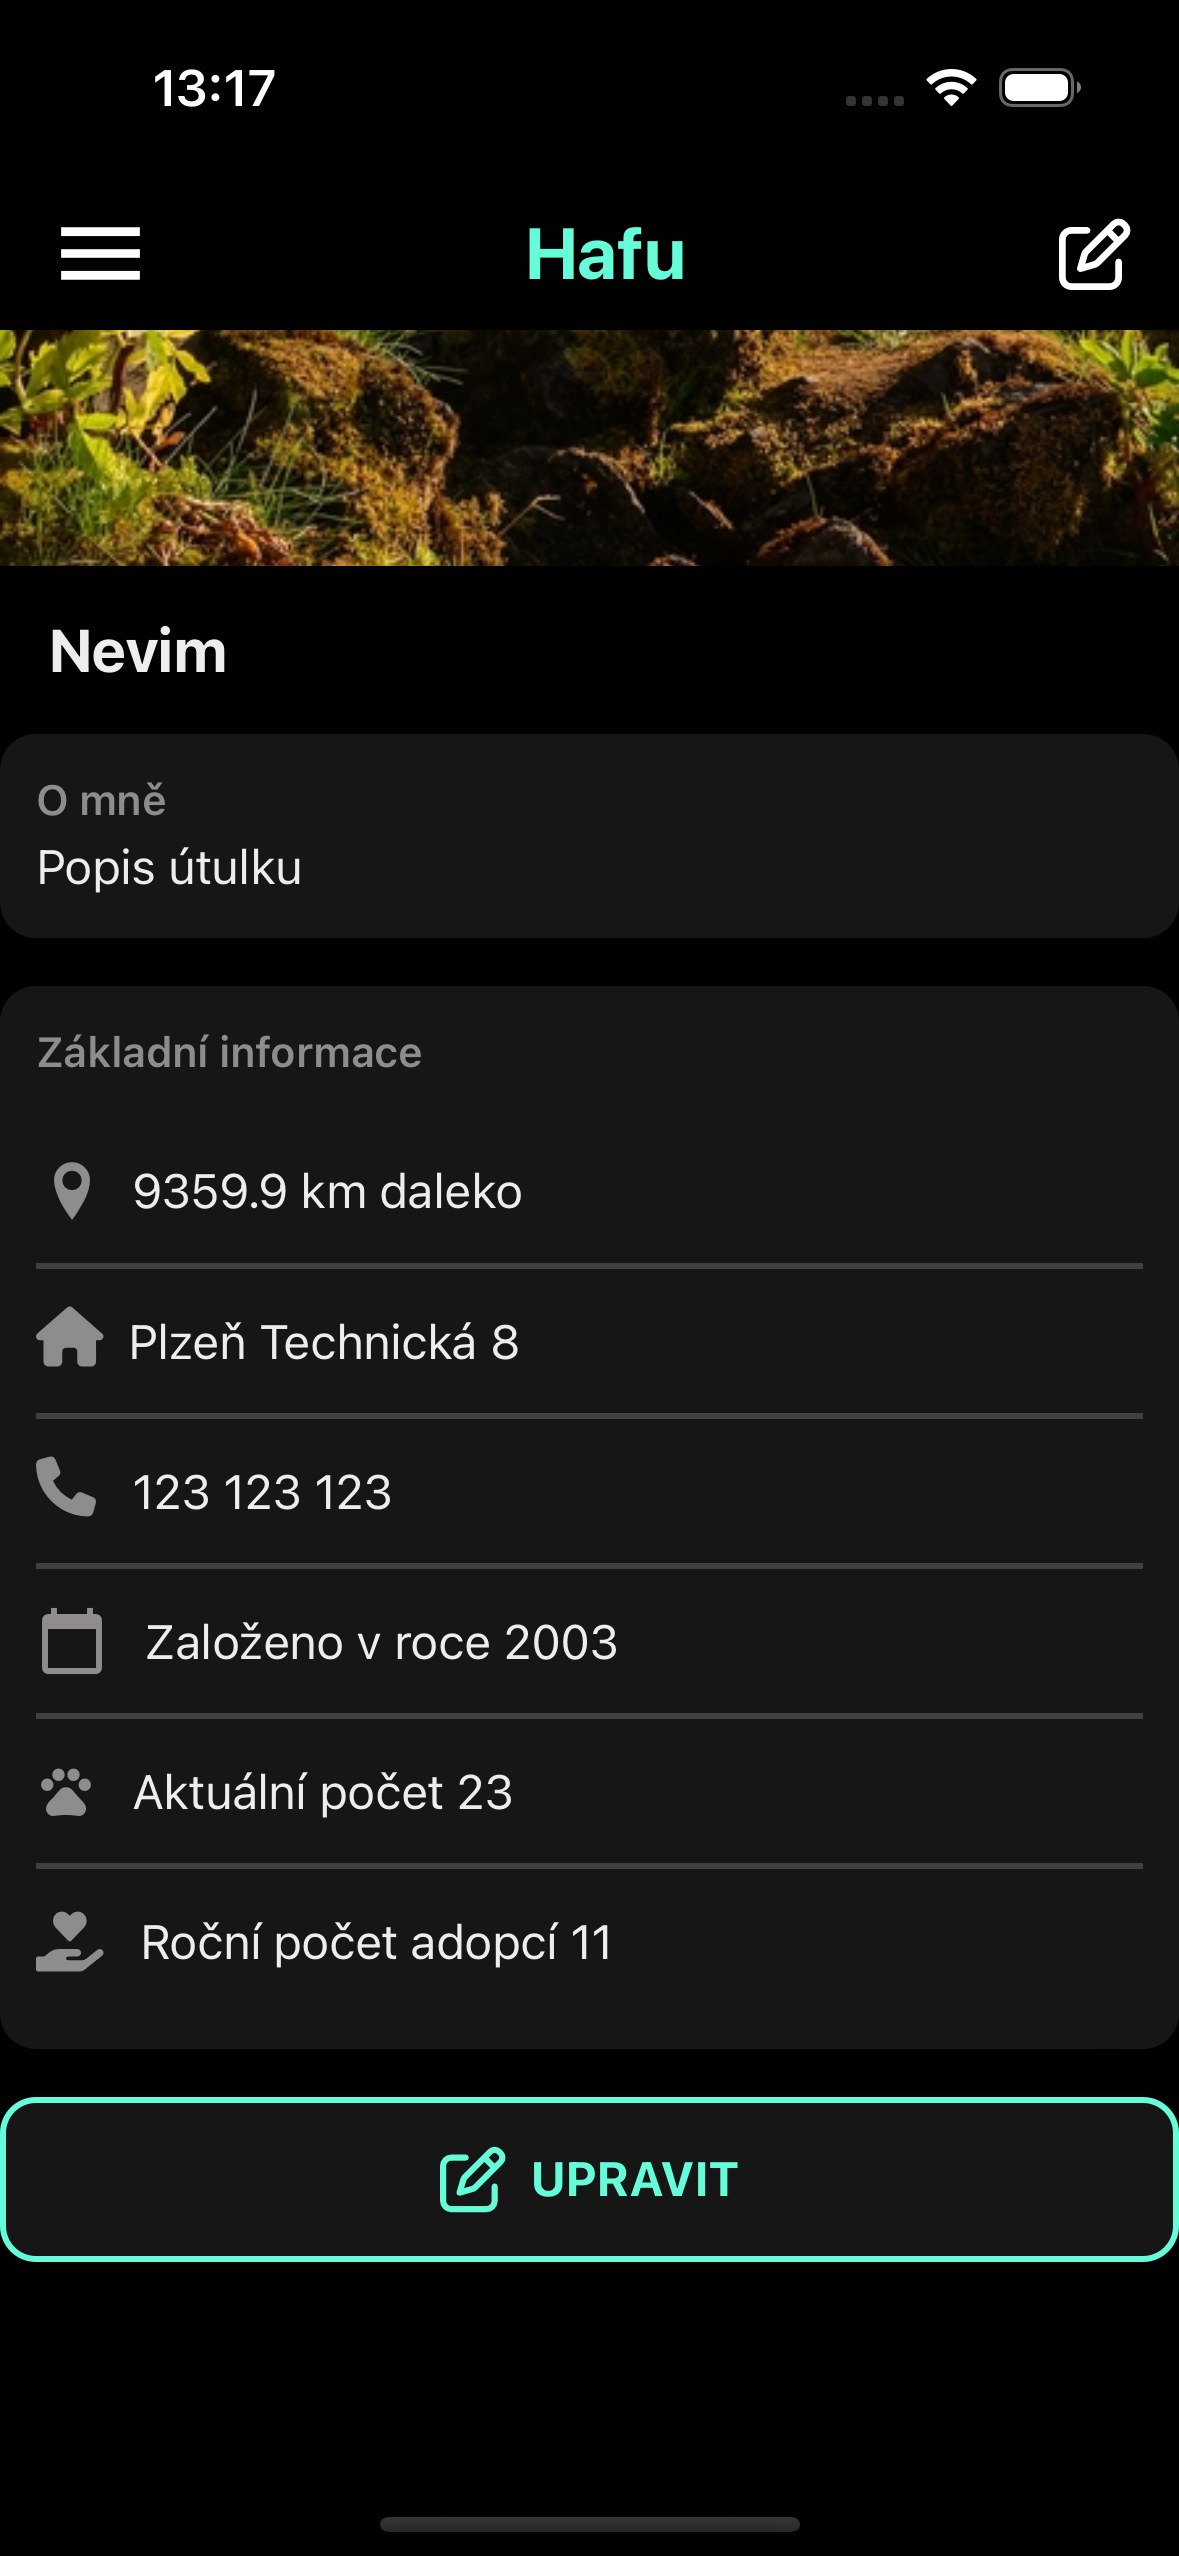
\includegraphics[width=\textwidth]{img-bp/shelterDetail.png} 
        \caption{Detail útulku}
        \label{fig:shelter-detail-uz}
    \end{subfigure}
    \hspace{0.03\textwidth}
    \begin{subfigure}{0.3\textwidth}
        \centering
        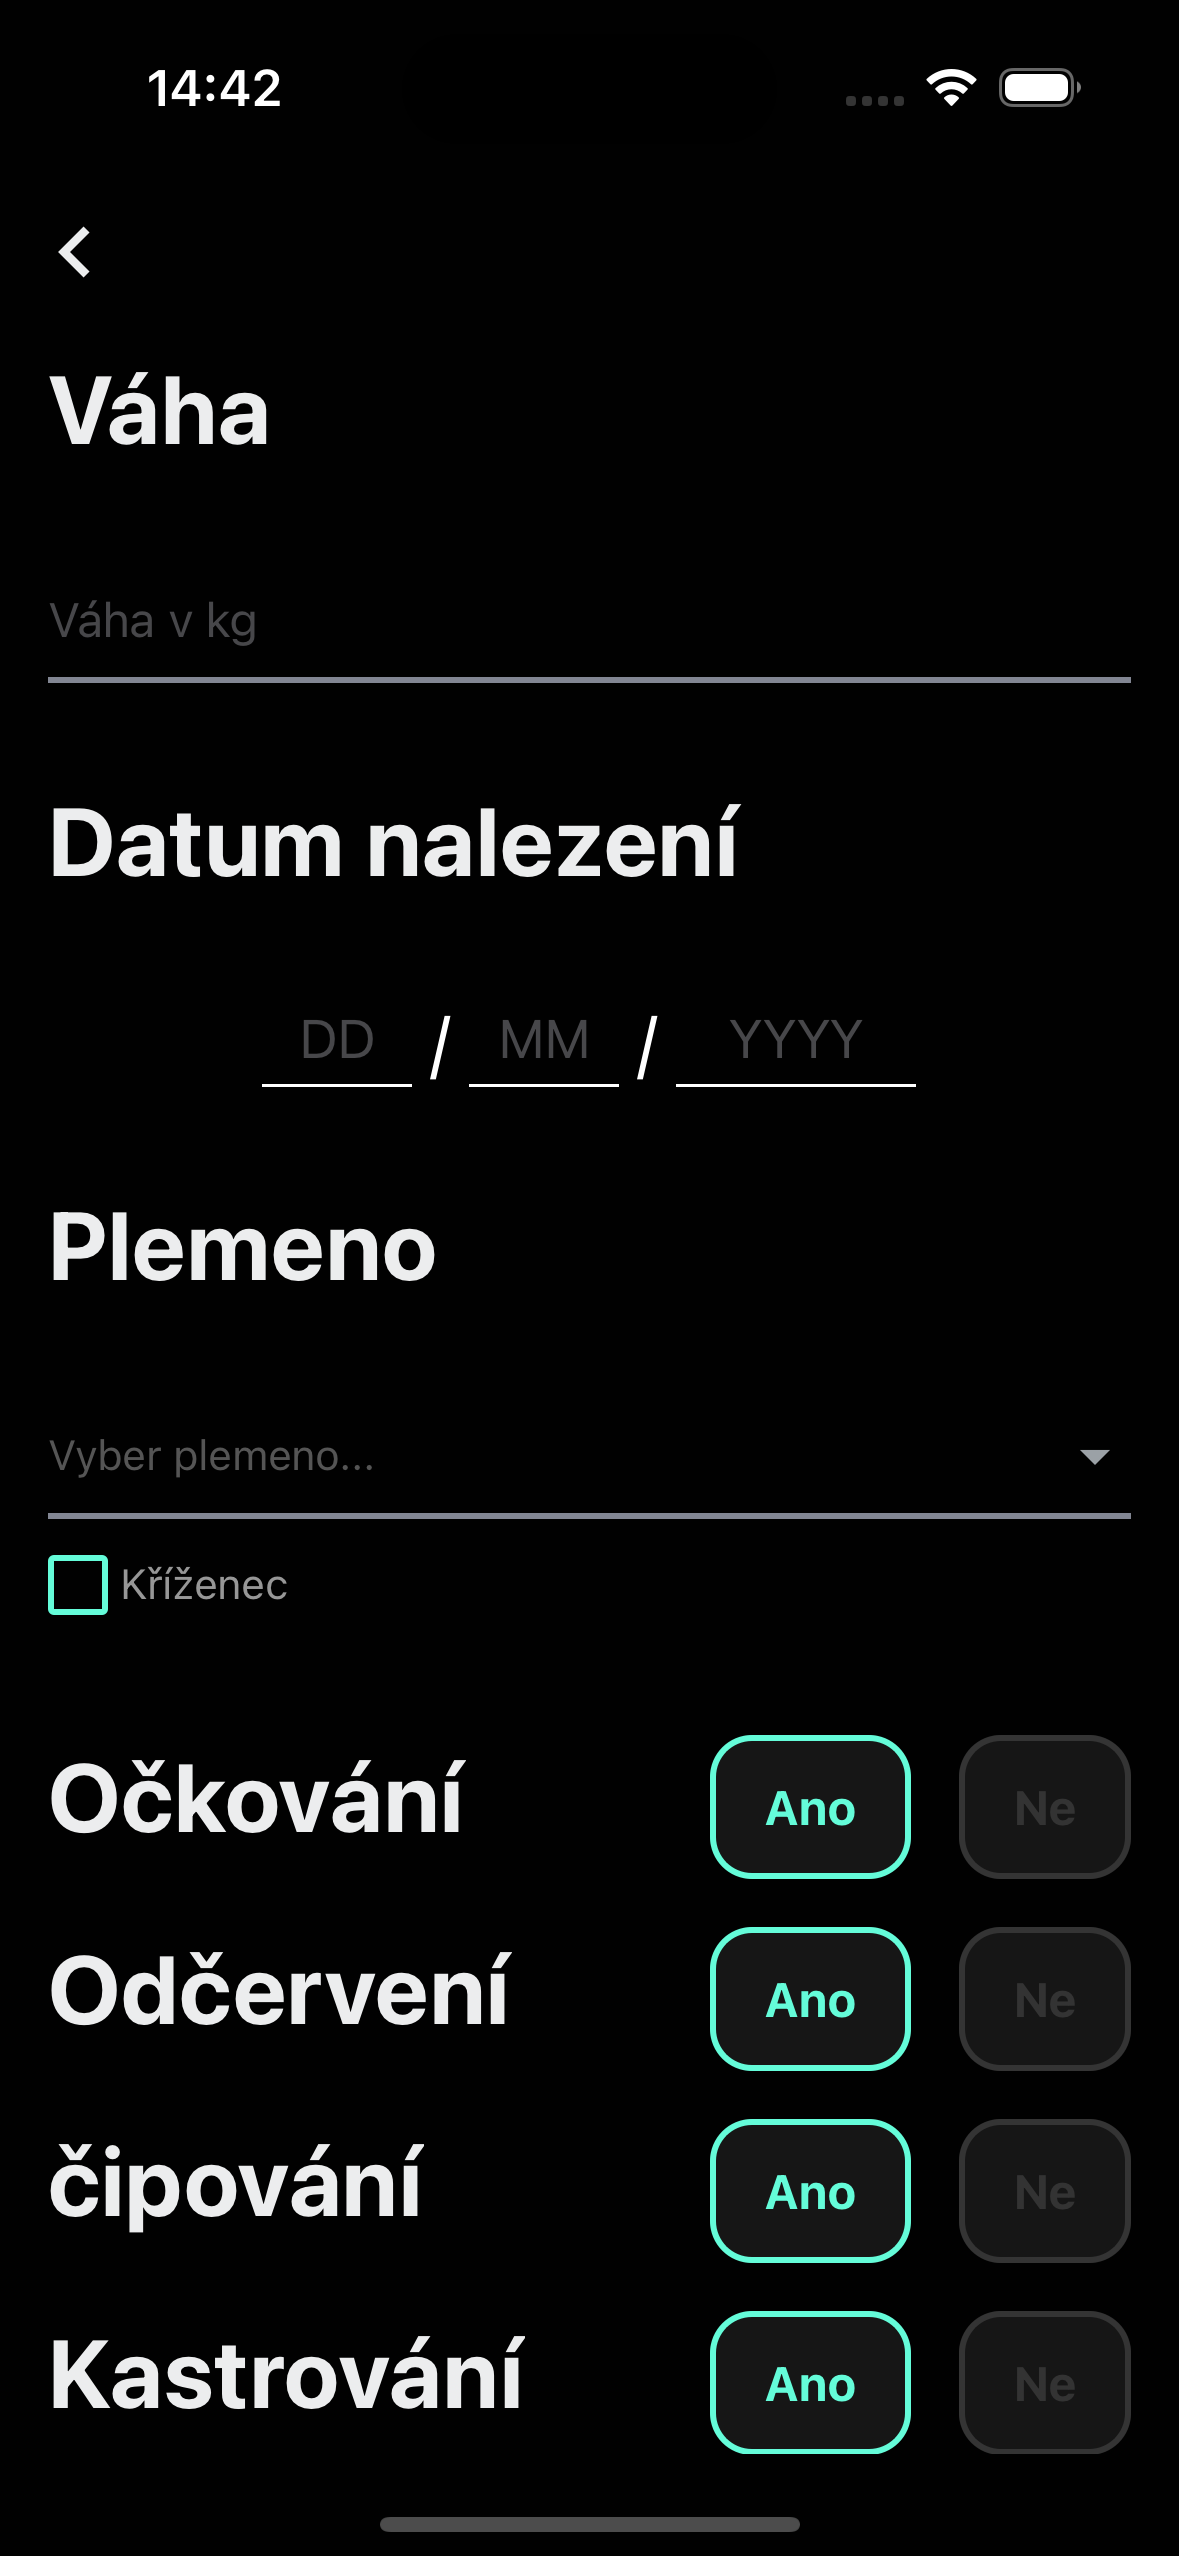
\includegraphics[width=\textwidth]{img-bp/petAdd.png} 
        \caption{Formulář zvířete}
        \label{fig:pet-add-uz}
    \end{subfigure}
    \caption{Ukázky obrazovek z aplikace}
\end{figure}

\chapter{Struktura přiloženého zip souboru}
\label{chap:struktura-zip}

\dirtree{%
.1 Aplikace\_a\_knihovny\ldots\DTcomment{Tento soubor obsahuje spouštěcí scripty aplikace, knihovny a zdrojové soubory}.
.2 android\DTcomment{Obsahuje konfigurační soubory pro Android build}.
.2 app\DTcomment{Obsahuje hlavní zdrojové soubory aplikace}.
.2 assets\DTcomment{Obsahuje obrázky, fonty a další statické soubory}.
.2 components\DTcomment{Obsahuje znovupoužitelné komponenty aplikace}.
.2 constants\DTcomment{Obsahuje definice konstant používaných v aplikaci}.
.2 hooks\DTcomment{Obsahuje vlastní React hooks pro sdílení logiky}.
.2 ios\DTcomment{Obsahuje konfigurační soubory pro iOS build}.
.2 lib\DTcomment{Obsahuje vlastní knihovny}.
.2 scripts\DTcomment{Obsahuje pomocné skripty pro build a deployment}.
.2 utils\DTcomment{Obsahuje pomocné funkce a utility}.
.1 Text\_prace\DTcomment{Text bakalářské práce}.
.1 Readme.txt\DTcomment{Popis struktury přiloženého zip souboru}.
}

\printbibliography

\chapter*{Seznam zkratek}

\begin{tabular}{ll}
\textbf{AAA} & Arrange Act Assert \\
\textbf{API} & Application Programming Interface \\
\textbf{AWS} & Amazon Web Services \\
\textbf{CLI} & Command Line Interface \\
\textbf{CPU} & Central Processing Unit \\
\textbf{CSS} & Cascading Style Sheets \\
\textbf{E2E} & End-to-end \\
\textbf{EAS} & Expo Application Services \\
\textbf{GDPR} & General Data Protection Regulation \\
\textbf{GPS} & Global Positioning System \\
\textbf{HIPAA} & Health Insurance Portability and Accountability Act \\
\textbf{HTTP} & HyperText Transfer Protocol \\
\textbf{HTTPS} & HyperText Transfer Protocol Secure \\
\textbf{JPG} & Joint Photographic Experts Group \\
\textbf{JSON} & JavaScript Object Notation \\
\textbf{NoSQL} & Not only SQL \\
\textbf{OTP} & One-time Password \\
\textbf{PNG} & Portable Network Graphic \\
\textbf{RAM} & Random-access Memory \\
\textbf{ReactDOM} & React Document Object Model \\
\textbf{REST} & Representational State Transfer \\
\textbf{S3} & Amazon Simple Storage Service \\
\textbf{SDK} & Service Development Kit \\
\textbf{SOC-2} & Service Organization Control 2 \\
\textbf{SQL} & Structured Query Language \\
\textbf{UI} & User Interface \\
\textbf{URL} & Uniform Resource Locator \\
\textbf{UX} & User experience \\
\end{tabular}

\listoffigures
\listoftables

\backmatter
\setbackpageqrcode
\backpage
\end{document}
